%!TEX TS-program = pdflatex
% dissertation.tex -- main dissertation file
%
% Wisconsin dissertation template
% Copyright (c) 2008-2009 William C. Benton.  All rights reserved.
%
% This program can redistributed and/or modified under the terms
% of the LaTeX Project Public License Distributed from CTAN
% archives in directory macros/latex/base/lppl.txt; either
% version 1 of the License, or (at your option) any later version.
%
% This program includes other software that is licensed under the
% terms of the LPPL and the Perl Artistic License; see README for details.
%
% You, the user, still hold the copyright to any document you produce
% with this software (like your dissertation).
%
\PassOptionsToPackage{dvipsnames}{xcolor} % prevent an option clash
% Comment to insert real images
\PassOptionsToPackage{draft}{graphicx}

%%% You'll want ``oneside'' for the deposit version, but probably not for any versions that don't need to meet the UW requirements
\documentclass[12pt,oneside,letterpaper]{memoir}

% preamble.tex -- packages to include
%
% Wisconsin dissertation template
% Copyright (c) 2008 William C. Benton.  All rights reserved.
%
% This program can redistributed and/or modified under the terms
% of the LaTeX Project Public License Distributed from CTAN
% archives in directory macros/latex/base/lppl.txt; either
% version 1 of the License, or (at your option) any later version.
%
% This program includes other software that is licensed under the
% terms of the LPPL and the Perl Artistic License; see README for details.
%
% You, the user, still hold the copyright to any document you produce
% with this software (like your dissertation).

%% You should use natbib
\IfFileExists{natbib.sty}{%
\usepackage[authoryear]{natbib}%
}{}

\usepackage[margin=1in]{geometry}
\ifpdf
\usepackage[pdftex]{graphicx}
\else
\usepackage{graphicx}
\fi
\usepackage{pdflscape}
\usepackage{rotating}
%% You probably need appendix, if you want appendices
\IfFileExists{appendix.sty}{%
\usepackage{appendix}%
}{}


%% the spacing in memoir is weird, you'll need to use this
\DisemulatePackage{setspace}
%% \usepackage[onehalfspacing]{setspace}
\usepackage[doublespacing]{setspace}

%% List setup; the ``hanglist`` environment will allow you to have
%% nicely-typeset enumerated lists (i.e. with the numbers hanging in
%% the margins).  You need at least version 2.1 of enumitem.sty.  If
%% you don't have enumitem installed at all, hanglist will just be an
%% alias for enumerate.
\IfFileExists{enumitem.sty}{%
\usepackage[loadonly]{enumitem}[2007/06/30]%
\newlist{hanglist}{enumerate}{1}% 
\setlist[hanglist]{label=\arabic*.}%
\setlist[hanglist,1]{leftmargin=0pt}%
}{%
\newenvironment{hanglist}{\begin{enumerate}}{\end{enumerate}}%
}


%% Avoid ugly "Type 3" fonts
\usepackage{lmodern}
\usepackage[LY1]{fontenc}
\usepackage[LY1]{eulervm}
%% Comment out any of these that you don't want
\usepackage{amssymb}
\usepackage{amsmath}
\usepackage{amsthm}
\usepackage{bm}
%\usepackage{theorem}
\usepackage{hyperref}
\usepackage[dvipsnames]{xcolor}
\usepackage{wrapfig}
\usepackage[nonumberlist,xindy,toc]{glossaries}

\usepackage{algorithm}
\usepackage[noend]{algpseudocode}
\usepackage{color}
\usepackage{framed}
\definecolor{shadecolor}{gray}{0.9}

\algnewcommand{\algorithmicreshape}{\textbf{reshape}}%
\algnewcommand{\Reshape}{\algorithmicreshape~}%

\algnewcommand{\algorithmicrecompute}{\textbf{compute}}%
\algnewcommand{\Compute}{\algorithmicrecompute~}%

\algnewcommand{\algorithmicreset}{\textbf{set}}%
\algnewcommand{\Set}{\algorithmicreset~}%

\renewcommand{\algorithmicrequire}{\textbf{Input:}}
\renewcommand{\algorithmicensure}{\textbf{Output:}}

\usepackage{multirow}
\usepackage{array}
\usepackage{booktabs}
\usepackage{comment}
\usepackage{forest}
\usepackage{float}

\newcommand{\tr}{\ensuremath{\mbox{tr}}}
\newcommand{\str}{\ensuremath{\mbox{\small tr}}}
\newcommand{\bvec}[1]{\hbox{\boldmath $#1$}}
\newcolumntype{C}[1]{>{\centering\let\newline\\\arraybackslash\hspace{0pt}}m{#1}}


\definecolor{light-gray}{gray}{.9}
\definecolor{dark-gray}{gray}{0.60}

\newcommand{\reducedstrut}{\vrule width 0pt height .9\ht\strutbox depth .9\dp\strutbox\relax}
\newcommand{\chighlight}[1]{%
  \begingroup
  \setlength{\fboxsep}{.5pt}%  
  \colorbox{light-gray}{\reducedstrut#1\/}%
  \endgroup
}

\usepackage{tikz}
\usetikzlibrary{decorations.pathreplacing,calc}
\newcommand{\tikzmark}[1]{\tikz[overlay,remember picture] \node (#1) {};}

\newcommand*{\AddNote}[4]{%
    \begin{tikzpicture}[overlay, remember picture]
        \draw [decoration={brace,amplitude=0.5em},decorate,ultra thick,red]
            ($(#3)!(#1.north)!($(#3)-(0,1)$)$) --  
            ($(#3)!(#2.south)!($(#3)-(0,1)$)$)
                node [align=center, text width=2.5cm, pos=0.5, anchor=west] {#4};
    \end{tikzpicture}
}%


\IfFileExists{mathpartir.sty}{%
\usepackage{mathpartir}%
}{}

%%%%% LISTINGS package and setup
\IfFileExists{listings.sty}{%
\usepackage{listings}%
}{}



%% Get rid of ugly borders around PDF hyperlinks (e.g. for cross-references, bib entries, or URLs)
\hypersetup{pdfborder = 0 0 0}

%% You want microtype.
\IfFileExists{microtype.sty}{%
\usepackage[protrusion=true,expansion=true]{microtype}%
}{}

%\pagestyle{thesisdraft}

\usepackage{afterpage}

% Surround parts of graphics with box
\usepackage{boxedminipage}

%% booktabs (thx to Nate Rosenblum for bringing this beautiful package
%% to my attention)
\IfFileExists{booktabs.sty}{%
\usepackage{booktabs}%
}{}

% This is now the recommended way for checking for PDFLaTeX:
\usepackage{ifpdf}



%% Substitute your favorite serif and sans fonts here....
%\IfFileExists{tgpagella.sty}{%
% TeX Gyre pagella, like Palatino
%\usepackage{tgpagella}%
%}{}

\usepackage{ifthen}

\providecommand\pdfforprinting{true}

\ifthenelse{\equal{\pdfforprinting}{false}}{%
\newenvironment{myrotatedtable}{%
  \newgeometry{margin=1cm}%
  \landscape%
  \table[p]%
}{%
  \endtable%
  \endlandscape%
  \restoregeometry%
}%
}{%
\newenvironment{myrotatedtable}{%
    \begin{sidewaystable}%
}{%
    \end{sidewaystable}
}%
}%

\usepackage{makeidx}
\makeindex
\makeglossaries

{\theoremstyle{plain}
\newtheorem{thm}{Theorem}[chapter]
\newtheorem{cor}[thm]{Corollary}
\newtheorem{define}[thm]{Definition}
\newtheorem{exmpl}[thm]{Example}
}
{\theoremstyle{remark}
\newtheorem{rmk}[thm]{Remark}
}

\newtheoremstyle{customsty1}
{3pt}%
{3pt}%
{}% --- body font
{}% --- indent amount
{\bfseries}% --- Theorem head font
{:}% --- Punctuation after head
{.5em}% --- space after head
{}% --- theorem head spec (can be left empty, meaning 'normal')

% Define 'newtheorems' that use ``customsty1''
{\theoremstyle{customsty1} 
}

% Some helper commands used in original source documents
\newcommand{\newtext}[1]{#1}
\newcommand{\oldtext}[1]{}
\newcommand{\newmath}[1]{\ensuremath{#1}}
\newcommand{\oldmath}[1]{}
\newcommand{\addedfragile}[1]{#1}
\renewcommand{\changed}[2]{\newtext{#1}\oldtext{#2}}




%%% NB: the ``deposit'' chapter- and page- styles should conform to UW
%%% requirements.  If you are producing a pretty version of your
%%% dissertation for web use later, you will certainly want to make
%%% your own chapter and page styles.

\makechapterstyle{deposit}{%
  \renewcommand{\chapterheadstart}{}
  \renewcommand{\printchaptername}{}
  \renewcommand{\chapternamenum}{}
  \renewcommand{\printchapternum}{\parbox{2em}{\MakeLowercase{\Large\scshape\thechapter{}}} }
  \renewcommand{\afterchapternum}{}
  \renewcommand{\printchaptertitle}[1]{%
  \raggedright\Large\scshape\MakeLowercase{##1}}
  \renewcommand{\afterchaptertitle}{%
  \vskip\onelineskip \hrule\vskip\onelineskip}
}

\makepagestyle{deposit}
 
\makeatletter
 
\renewcommand{\chaptermark}[1]{\markboth{#1}{}}
\renewcommand{\sectionmark}[1]{\markboth{#1}{}}
 
\makeevenfoot{deposit}{}{}{}
\makeoddfoot{deposit}{}{}{}
\makeevenhead{deposit}{\thepage}{}{}
\makeoddhead{deposit}{}{}{\thepage}
\makeatother

%%% set up page numbering for chapter pages to satisfy UW requirements
%%% NB: You will want to delete until the ``SNIP'' mark if you are
%%% making a ``nice'' copy
\copypagestyle{chapter}{plain}
\makeoddfoot{chapter}{}{}{}
\makeevenhead{chapter}{\thepage}{}{}
\makeoddhead{chapter}{}{}{\thepage}
%%% SNIP

%%% bib nonsense
\makeatletter
\newenvironment{wb-bib}[1]{%
  \chapter*{references}
\ifnobibintoc\else 
\phantomsection 
\addcontentsline{toc}{chapter}{References} 
\fi 
\prebibhook
  \begin{bibitemlist}{#1}}{\end{bibitemlist}\postbibhook}

\AtBeginDocument{%
  \@ifpackageloaded{natbib}{% natbib is loaded
    \addtodef{\endthebibliography}{}{\vskip-\lastskip\postbibhook}
    \@ifpackagewith{natbib}{sectionbib}{% with sectionbib option
      \renewcommand{\bibsection}{\@memb@bsec}}%
      {\renewcommand{\bibsection}{\@memb@bchap}}}%
  {}
  \@ifpackagewith{chapterbib}{sectionbib}{%
    \renewcommand{\sectionbib}[2]{}
    \renewcommand{\bibsection}{\@memb@bsec}}{}
}
\makeatother


\renewcommand{\sc}{\scshape}

%%% Local Variables:
%%% mode: latex
%%% TeX-master: "../document"
%%% End:

\input{includes/defs}
\input{includes/thesisdefs}
\newacronym[%
description={A Practical Visual Interactive System is a dynamic
virtual environment where by user input produces changes in state for
the purpose of supporting some task.}]
{pvis}{PVIS}{practical visual interactive system}

\newacronym[%
description={A Head Mounted Display is a virtual reality display
  device that fits over a user's head, providing them with an isolated
  and personal immersive experience into virtual environments.}]
{hmd}{HMD}{head mounted display}

\newglossaryentry{tacit}{%
  description={Tacit Knowledge is knowledge which is difficult to
    communicate to others via direct methods, such as speaking or
    writing. Examples might include how to play an instrument or playing
    a sport.},
  name={tacit knowledge}
}

\newglossaryentry{psymotor}{%
  description={Psychomotor skills are skills that require extensive coordination between the physical body and mental processes. Examples include playing an instrument or physically manipulating surgical tools during surgery.},
  name={psychomotor skill}
  }

\newglossaryentry{deformablesolid}{%
description={A deformable solid is a volumetric region whose shape reacts to both internal mechanics and external stimuli},
name={deformable solid}
}

\newglossaryentry{hyperelastic}{%
description={A hyperelastic material is a material whose strain energy does not depend on the history of past deformations the material has undergone. While idealized and not found in nature, these materials are often described as rubber-like, as rubber and similar real materials are very hyperelastic in their behavior under low stress loads.},
name={hyperelastic}
}

\newglossaryentry{plasticity}{%
description={A plastic material is a material which incorporates previous deformation history when computing the current deformation strain energy. This gives rise to persistent effects like creasing and shape-holding after bends. Common materials with plasticity effects include most metals, paper, and some plastics.},
name={plasticity}
}

\newacronym[%
description={The Finite Element Method is a type of computational analysis of materials which utilizes a number of discrete regions or elements to describe a larger region of material. By using the relatively simple behaviors of each element, a vastly more complex of the whole material can be derived.}]
{fem}{FEM}{Finite Element Method}
%\usepackage[noend]{algcompatible}
\usepackage{algorithm}
\usepackage[noend]{algpseudocode}
\usepackage{tikz}
\usetikzlibrary{calc}
\algnewcommand\algorithmicgoto{\textbf{goto: }}
\algnewcommand\Goto{\algorithmicgoto}
\algrenewcommand\algorithmicindent{0.5em}%
\algnewcommand{\LineComment}[1]{\State {\color{NavyBlue} \(\triangleright\) \textbf{#1}}}

\usepackage{caption}% http://ctan.org/pkg/caption
\captionsetup[ruled]{labelsep=colon}
\makeatletter
\@addtoreset{algorithm}{chapter}% algorithm counter resets every chapter
\makeatother
\renewcommand{\thealgorithm}{\thechapter.\arabic{algorithm}}% Algorithm # is <chapter>.<algorithm>


\makeatletter
\newcommand{\StatexIndent}[1][3]{%
  \setlength\@tempdima{\algorithmicindent}%
  \Statex\hskip\dimexpr#1\@tempdima\relax}
\algdef{S}[IF]{IfNoThen}[1]{\algorithmicif\ #1}%
\makeatother

\makeatletter
\tikzset{%
  remember picture with id/.style={%
    remember picture,
    overlay,
    save picture id=#1,
  },
  save picture id/.code={%
    \edef\pgf@temp{#1}%
    \immediate\write\pgfutil@auxout{%
      \noexpand\savepointas{\pgf@temp}{\pgfpictureid}}%
  },
  if picture id/.code args={#1#2#3}{%
    \@ifundefined{save@pt@#1}{%
      \pgfkeysalso{#3}%
    }{
      \pgfkeysalso{#2}%
    }
  }
}

\def\savepointas#1#2{%
  \expandafter\gdef\csname save@pt@#1\endcsname{#2}%
}

\def\tmk@labeldef#1,#2\@nil{%
  \def\tmk@label{#1}%
  \def\tmk@def{#2}%
}

\tikzdeclarecoordinatesystem{pic}{%
  \pgfutil@in@,{#1}%
  \ifpgfutil@in@%
    \tmk@labeldef#1\@nil
  \else
    \tmk@labeldef#1,(0pt,0pt)\@nil
  \fi
  \@ifundefined{save@pt@\tmk@label}{%
    \tikz@scan@one@point\pgfutil@firstofone\tmk@def
  }{%
  \pgfsys@getposition{\csname save@pt@\tmk@label\endcsname}\save@orig@pic%
  \pgfsys@getposition{\pgfpictureid}\save@this@pic%
  \pgf@process{\pgfpointorigin\save@this@pic}%
  \pgf@xa=\pgf@x
  \pgf@ya=\pgf@y
  \pgf@process{\pgfpointorigin\save@orig@pic}%
  \advance\pgf@x by -\pgf@xa
  \advance\pgf@y by -\pgf@ya
  }%
}


% end of Andrew's code

\newlength\AlgIndent
\setlength\AlgIndent{0pt}
% main command to draw the colored background
\newcounter{mymark}
\newcommand\ColorLine{%
  \stepcounter{mymark}%
  \tikz[remember picture with id=mark-\themymark,overlay] {;}%
  \begin{tikzpicture}[remember picture,overlay]%
    \filldraw[YellowGreen]%
   let \p1=(pic cs:mark-\themymark),
   \p2=(pic cs:mark-\themymark) in 
   ([xshift=-\ALG@thistlm,yshift=-0.7ex]0,\y1)  rectangle ++(\linewidth+.1em,\baselineskip);
  \end{tikzpicture}%
}%
\makeatother

% colored loops and declarations
\makeatletter
\algnewcommand\CREQUIRE{\item[\setlength\AlgIndent{1.6em}\ColorLine\algorithmicrequire]}%
\algnewcommand\CENSURE{\item[\setlength\AlgIndent{1.6em}\ColorLine\algorithmicensure]}%
\algnewcommand\CSTATE{\State\ColorLine}%
\algnewcommand\CSTATEx{\Statex\ColorLine}%
\algnewcommand\CCOMMENT{\Comment\ColorLine}%

\algdef{SE}[WHILE]{CWHILE}{CENDWHILE}%
   [2][default]{\ColorLine\algorithmicwhile\ #2\ \algorithmicdo #1}%
   {\ColorLine\algorithmicend\ \algorithmicwhile}%
\algdef{SE}[FOR]{CFOR}{CENDFOR}%
   [2][default]{\ColorLine\algorithmicfor\ #2\ \algorithmicdo #1}%
   {\ColorLine\algorithmicend\ \algorithmicfor}%
\algdef{SE}[FOR]{CFORALL}{CENDFORALL}%
   [2][default]{\ColorLine\algorithmicforall\ #2\ \algorithmicdo #1}%
   {\vspace{-\baselineskip}%\algorithmicend\ \algorithmicfor
}%
\algdef{SE}[FOR]{FORALL}{ENDFORALL}%
   [2][default]{\algorithmicforall\ #2\ \algorithmicdo #1}%
   {\algorithmicend\ \algorithmicfor}%
\algdef{SE}[LOOP]{CLOOP}{CENDLOOP}%
   [1][default]{\ColorLine\algorithmicloop #1}%
   {\ColorLine\algorithmicend\ \algorithmicloop}%
\algdef{SE}[REPEAT]{CREPEAT}{CUNTIL}%
   [1][default]{\ColorLine\algorithmicrepeat #1}%
   [1]{\ColorLine\algorithmicuntil\ #1}%
\algdef{SE}[IF]{CIF}{CENDIF}%
   [2][default]{\ColorLine\algorithmicif\ #2\ \algorithmicthen #1}%
   {\vspace{-\baselineskip}%\algorithmicend\ \algorithmicif
}%
\algdef{C}[IF]{CIF}{CELSIF}%
   [2][default]{\ColorLine\algorithmicelse\ \algorithmicif\ #2\ \algorithmicthen #1}%
\algdef{Ce}[ELSE]{CIF}{CELSE}{CENDIF}%
   [1][default]{\ColorLine\algorithmicelse #1}%



\makeatother

%%% Local Variables: 
%%% mode: latex
%%% TeX-master: "nonmanifold_levelsets"
%%% End: 


\svnidlong{$LastChangedBy$}{$LastChangedRevision$}{$LastChangedDate$}{$HeadURL: http://freevariable.com/dissertation/branches/diss-template/dissertation.tex $} 

\clearpage\pagenumbering{roman}  % This makes the page numbers Roman (i, ii, etc)

\title{Techniques for Single System Integration of Elastic Simulation Features}
\author{Nathan M. Mitchell}
\department{Computer Sciences}

\date{\the\year}

\begin{document}

%%% Uncomment the following if your .bib contains references that you will not 
%%% explicitly cite, but that should be in the final bibliography:
% \nocite{*}

\ifpdf
\DeclareGraphicsExtensions{.pdf, .jpg, .tif}
\else
\DeclareGraphicsExtensions{.eps, .jpg}
\fi

\maketitle

%% Add \part declarations if you want, but it's not necessary
%\part{Preliminaries}

\svnidlong{$LastChangedBy$}{$LastChangedRevision$}{$LastChangedDate$}{$HeadURL: http://freevariable.com/dissertation/branches/diss-template/frontmatter/frontmatter.tex $}
\vcinfo{}

%%% SOME OF THIS CODE IS ADAPTED FROM THE VENERABLE withesis.cls

% COPYRIGHT PAGE
%  - To include a copyright page use \copyrightpage
\copyrightpage

% DEDICATION
\begin{dedication}
  \emph{For my grandfather,\\ whose lifelong passion for teaching others\\ inspired me to
    pursue my own goals and education.}\\
  \vspace*{3cm}
  \includegraphics[width=4cm]{frontmatter/dahlia.png}
\end{dedication}

%% BEGIN PAGESTYLE

%%% You can pick a pagestyle if you want; see the memoir class
%%% documentation for more info.  The default ``deposit'' option meets
%%% the UW thesis typesetting requirements but is probably
%%% unsatisfactory for making a version of your dissertation that
%%% won't be deposited to the graduate school (e.g. for web or a nice
%%% printed copy)

\chapterstyle{deposit}
\pagestyle{deposit}


% ACKNOWLEDGMENTS
\begin{acks}

I would like to thank all the people who have
supported me and my work over the years. In
particular, I would like to thank my family who
have shown me unwavering support and my friends
who have kept me sane. Also, I would like to thank
Ben Recht, Ronald Fedkiw, Matthew Cong for their
advice and discussions on several of the
contributions made in this
dissertation. Additionally, I wish to extend my
thanks to Dr. Timothy King, the medical residents
of the Plastic \& Reconstructive Surgery program,
and the School of Medicine and Public Health at
the University of Wisconsin-Madison for their
involvement and support with the virtual plastic
surgery platform, as well as acknowledge Aaron
Oliker and BioDigital Systems for supplying the
models used in this project.

This work was generously supported by the following grants
and funding sources: NSF grants IIS-1253598,
IIS-1407282, CCF-1423064, CCF-1533885,
CNS-1218432, CCF-1438992.


%%% Local Variables: 
%%% mode: latex
%%% TeX-master: "../dissertation"
%%% End: 

\end{acks}

% CONTENTS, TABLES, FIGURES
\renewcommand{\printtoctitle}[1]{\chapter*{#1}}
\renewcommand{\printloftitle}[1]{\chapter*{#1}}
\renewcommand{\printlottitle}[1]{\chapter*{#1}}

\renewcommand{\tocmark}{}
\renewcommand{\lofmark}{}
\renewcommand{\lotmark}{}

\renewcommand{\tocheadstart}{}
\renewcommand{\lofheadstart}{}
\renewcommand{\lotheadstart}{}

\renewcommand{\aftertoctitle}{}
\renewcommand{\afterloftitle}{}
\renewcommand{\afterlottitle}{}

\renewcommand{\cftchapterfont}{\normalfont} 
\renewcommand{\cftsectionfont}{\itshape} 
\renewcommand{\cftchapterpagefont}{\normalfont} 
\renewcommand{\cftchapterpresnum}{\bfseries} 
%\renewcommand{\cftchapterleader}{\cftparfillskip} 
%\renewcommand{\cftsectionleader}{\cftparfillskip} 
%\renewcommand{\cftchapterafterpnum}{\cftparfillskip} 
%\renewcommand{\cftsectionafterpnum}{\cftparfillskip} 

% \captionnamefont{\small\sffamily} 
% \captiontitlefont{\small\sffamily} 

\renewcommand{\cftdot}{}

% \renewcommand{\contentsname}{contents}
% \renewcommand{\listfigurename}{list of figures}
% \renewcommand{\listtablename}{list of tables}

\addtocontents{toc}{~\hfill\textbf{Page}\par}
\tableofcontents

\clearpage
\listoftables
\addtocontents{lot}{~\hfill\textbf{Page}\par}

\clearpage
\listoffigures
\addtocontents{lof}{~\hfill\textbf{Page}\par}

\clearpage
\listofalgorithms
\addtocontents{loa}{~\hfill\textbf{Page}\par}
\addcontentsline{toc}{chapter}{List of Algorithms}


\clearpage
% NOMENCLATURE
% \begin{conventions}
% % \begin{description}
% % \item{\makebox[0.75in][l]{term}
% %        \parbox[t]{5in}{definition\\}}
% % \end{description}
% \input{conventions}
% \end{conventions}

%% The UW graduate school no longer wants a UMI abstract page
%% Should you need one for some reason, uncomment the following
%% lines.  Thanks to Matt Fredrikson for reporting this!

% \advisorname{Gottlob Frege}
% \advisortitle{Professor}
% \begin{umiabstract}
%  
Techniques for simulating the behavior of elastic objects has matured
considerably over the last several decades, tackling diverse problems
from non-linear models for incompressibility to accurate
self-collisions. Alongside these contributions, advances in parallel
hardware design and algorithms have made simulation more efficient and
affordable than ever before. However, prior research has commonly made
the choice to sacrifice one aspect of simulation for another,
resulting in a fragmented landscape of solutions. For complex,
real-world tasks, such as virtual surgery, a holistic approach is
desirable, where complex behavior, performance, and ease of modeling
are supported equally. This dissertation aims to provide that in the
form of several interconnected investigations, each of which
contribute a piece of an unified solution. First, it will be
demonstrated how advanced non-linear materials can be combined with
lattice deformers yield simulations with behavioral richness and a
high potential for parallelism. This potential will be exploited to
show how a hybrid solver approach based on large macroblocks can
accelerate the convergence of these deformers. Extending the lattice
concept with non-manifold topology allows for efficient processing of
self-collisions and topology change. Finally, a case study on virtual
plastic surgery will demonstrate a real-world problem space where
these ideas can be combined to build an expressive authoring tool,
allowing surgeons to record procedures digitally for future reference
or education.


%%% Local Variables:
%%% mode: latex
%%% TeX-master: "../dissertation"
%%% End:

% \end{umiabstract}

\begin{abstract}
  
Techniques for simulating the behavior of elastic objects has matured
considerably over the last several decades, tackling diverse problems
from non-linear models for incompressibility to accurate
self-collisions. Alongside these contributions, advances in parallel
hardware design and algorithms have made simulation more efficient and
affordable than ever before. However, prior research has commonly made
the choice to sacrifice one aspect of simulation for another,
resulting in a fragmented landscape of solutions. For complex,
real-world tasks, such as virtual surgery, a holistic approach is
desirable, where complex behavior, performance, and ease of modeling
are supported equally. This dissertation aims to provide that in the
form of several interconnected investigations, each of which
contribute a piece of an unified solution. First, it will be
demonstrated how advanced non-linear materials can be combined with
lattice deformers yield simulations with behavioral richness and a
high potential for parallelism. This potential will be exploited to
show how a hybrid solver approach based on large macroblocks can
accelerate the convergence of these deformers. Extending the lattice
concept with non-manifold topology allows for efficient processing of
self-collisions and topology change. Finally, a case study on virtual
plastic surgery will demonstrate a real-world problem space where
these ideas can be combined to build an expressive authoring tool,
allowing surgeons to record procedures digitally for future reference
or education.


%%% Local Variables:
%%% mode: latex
%%% TeX-master: "../dissertation"
%%% End:

\end{abstract}

\clearpage\pagenumbering{arabic}

%%% END STUFF TAKEN FROM WITHESIS EXAMPLE FILE

%%% Local Variables:
%%% mode: latex
%%% TeX-master: "../dissertation"
%%% End:


%%%%%%%%%%%%%%%%%%%%%%%%%%%%%%%%%%%%%%%%%%%%%%%%%%%%%%%%%%%%%%%%%%%%%%%% 
%%%%%%%%%%%%%%%%%%%%%%%%%%%%%%%%%%%%%%%%%%%%%%%%%%%%%%%%%%%%%%%%%%%%%%%%
%%%%%%%%%%%%%%%%%%%%%%%%%%%%%%%%%%%%%%%%%%%%%%%%%%%%%%%%%%%%%%%%%%%%%%%%
%                         INTRO CHAPTERS
%%%%%%%%%%%%%%%%%%%%%%%%%%%%%%%%%%%%%%%%%%%%%%%%%%%%%%%%%%%%%%%%%%%%%%%%
%%%%%%%%%%%%%%%%%%%%%%%%%%%%%%%%%%%%%%%%%%%%%%%%%%%%%%%%%%%%%%%%%%%%%%%%
%%%%%%%%%%%%%%%%%%%%%%%%%%%%%%%%%%%%%%%%%%%%%%%%%%%%%%%%%%%%%%%%%%%%%%%%

\chapter{Introduction}

Physicians have been seeking better methods to capture human anatomy and
its pathologies for the purpose of healing since the earliest days of
modern surgical theory. From the anatomical drawings of De Vinci, to more
modern practices of constructing realistic simulacra, surgeons, and
their students, have been pursuing tools that allow them to practice
their skills before operating on real patients. Existing research
shows the benefits of engaging in these practice
sessions~\citep{GallaRCHFMSS:2005}. Practiced surgeons make fewer
mistakes and can use preparation sessions to plan new approaches
safely.

This general philosophy, which can be summed up with the classic
proverb of ``measure twice, cut once'', is practiced by many high risk
professions. From flight school to driving simulators, computer
constructed virtual environments have become an integral part of
training highly skilled professionals. The reasoning is three-fold:
computer simulations are relatively low cost and are able to be reset
quickly, unforeseen parameters and situations can be introduced more easily
than physical environments, and a trainee's progress can be easily
recorded for later review. With these advantages over purely physical
training environments, why are surgeons still using aids such as
diagrams, physical mannequins, and cadavers?

The part of the answer is that they often lack any better
alternatives. Performing surgery is a complex task involving a
combination of dexterous and cognitive, often spatial reasoning,
skills~\citep{GallaRCHFMSS:2005}. Tools that support all of these areas
are difficult to get right, and most attempts to build technological
aids have focused on subsets of the skills required. Historically,
these have been the dexterous skills, which many authors have tried to
solve with a variety of haptic simulation
techniques~\citep{MendoL:2003, LindbT:2007}. While these surgical
simulation philosophies are useful, and have been used in commercial
products~\citep{SUSAC:2002--2014}, they don't really meet the need of
training cognitive skills. This need varies across surgical
specialties - reconstructive plastic surgery, which is the focus of this document,
requires the surgeon to have internalized geometrical intuitions in
order to manipulate tissue in the three dimensional space of the human
body. It is this lack that has kept traditional, less technological
aids as the core of many plastic surgery training programs.

In comparison to internal surgery, plastic surgery suffers from the
practical reality that the results of any operation will be visible to
others. This fact adds an additional constraint onto practitioners;
not only must their work be as technically correct as before, but they
must also be considering the final aesthetics of their procedures. It
follows then that a simulator for plastic surgery operations must
provide an environment for surgeons to freely practice design, as well
as correctly display the outcomes.

This dissertation aims to support the following statement: Creating
virtual simulators for craniofacial reconstructive plastic surgery has
reached the point of technical feasibility. This capability is
demonstrated using craniofacial reconstructive surgery as the
benchmark; both for its intrinsic value and the degree of complexity
and challenges it exemplifies. In pursuit of this goal, this document
will describe how current practices for simulating elastic materials
can be combined in a holistic fashion to optimize for performance and
practical usability. In the process, limitations with the current
approaches will be explored and, in some cases, alternative techniques
will be proposed to solve technical challenges that our benchmark
application exposes.


%%% Local Variables:
%%% mode: latex
%%% TeX-master: "../document"
%%% End:


\chapter{Motivation}
\label{chp:motivation}

In order to properly understand this dissertation, it is important to
place it the proper context. While the driving topic of this document
is simulation in the plastic surgery domain, the work presented here
in this dissertation derives from more fundamental motivations. The
goal of this chapter is to present a more complete motivation for the
design decisions and technical contributions presented throughout this
document.  In pursuit of this goal, this chapter will describe an
overarching framework for Practical Visual Interactive
Systems. Throughout, both high level design goals and challenges will
be discussed, along with specific examples which relate to plastic surgery.


\section{Practical Visual Interactive Systems}


At a high level, the work completed in support of this thesis falls under the description
of a \Gls{pvis}. A Practical Visual Interactive System \textit{is a dynamic
virtual environment where by user input produces changes in state for
the purpose of supporting some task}. These systems are actually
everywhere in our modern society, though we do not often think
of them in these terms. Examples include video games, virtual avatar
systems, training systems, and more. This section's goal is to define
what a \gls{pvis} is and is not. This deconstruction will be followed
by a examination of the challenges that exist when developing a
\gls{pvis} along with specific examples from plastic surgery
domain. Finally, a justification will be made, which will show that
\gls{pvis} development is warranted, despite the complexities involved.

\subsection{PVIS Deconstruction}

The core of a \gls{pvis} is a virtual world, or environment. The size
and scope of the environment is less important than the fact that the
environment \textit{is not real}. When discussing a \gls{pvis}, we are
talking about artificially constructed settings, often completely
described by a computer program and displayed via some
device. However, a \gls{pvis} is not completely disconnected from
reality. In order to support a user in a particular task, a \gls{pvis}
is often designed to mimic real life situations.

Returning to the definition above, is it appropriate to
declare any virtual environment a \gls{pvis}? Not exactly - a careful
reading of the proposed definition reveals that a \gls{pvis} is
structured according to a series of important properties, or \textit{aspects}.

\begin{description}
\item[Geometry] Most of the forms of \glspl{pvis} that people interact
  with today are displayed as 3D worlds. Full of rich and detailed 3D
  models, this environment type often is preferred when the goal is to
  recreate some aspect of actual reality. However, a \gls{pvis}'s
  environment should not be restricted to one in three dimensions. A
  designer should choose the environment's representation according to
  the utility they wish to extract from a \gls{pvis}. In addition to
  representation, it is also important to consider a \gls{pvis}'s
  interface. But whether a \gls{pvis} is designed around a standard
  desktop computer monitor, or a new virtual reality \gls{hmd}, it is
  important to prevent the choice of technology from overshadowing
  other aspects of the \gls{pvis}. The particular interface should be
  chosen with care in order to augment, not detract from, the utility of
  the system for its users.

\item[Reactivity] A \gls{pvis} should hold state and allow its
  users to change this state meaningfully via interactions with the system. This
  aspect critically enables many other useful properties of a
  \gls{pvis}. First, it brings an important property of determinism
  to the system. Instead of static or random reactions, users should
  expect their actions will produce understandable (yet not
  necessarily simple!) consequences. Second, this property defines the rules of
  the \gls{pvis}, which are important both to the designer and the
  user. The designer needs to understand the rules in order to make
  informed choices and compromises in development (more on this
  later). The user of the system needs the rules, even implicitly
  stated, to gain intuitions and learn how to use the system. If these
  rules faithfully replicate real world behaviors, the user may be
  able to translate knowledge learned from the \gls{pvis} into the
  physical world.
  
\item[Dynamism] Often conflated with the aspect of reactivity, dynamism
  brings in a temporal component to the \gls{pvis}. This moves the \gls{pvis} away
  from a what otherwise might be a simple state machine, whose states
  can be traversed in any order, to a system with a history. Whether
  this history property is permanent, where user input creates
  indelible changes to the virtual environment, or flexible, giving a
  user a timeline of consequences to move through at will, depends on the
  ultimate purpose of the \gls{pvis}. 

\item[Interactivity] While the aspects of reactivity and dynamism work
  together to create complex systems of internal state for a
  \gls{pvis}, they don't cover \textit{how} a user interacts with the
  system. While a movie could be construed as a very simple
  \gls{pvis}, whose state is the current frame and only dynamic
  behavior is to advance the frame, typically interacting with a
  \gls{pvis} is more semantically rich than a set of actions like
  play, pause and stop. More complex interactions can be found in
  advanced \glspl{pvis}, such as video games and training
  simulators. Here, interactions are designed to replicate the look
  and feel of real controls, or exist to immerse a user into the world
  by allowing them to embody a virtual character through movement or
  speech. These advanced modes serve to both increase the realism of
  the system and to give the user a more comfortable or familiar set
  of mental tools to think about the system with.

\item[Purpose] A \gls{pvis} without a purpose is not a \gls{pvis}. The
  \gls{pvis}'s purpose helps define what features are important and
  clarifies what metrics should be used to measure its ultimate
  success. All of the other aspects of a \gls{pvis} must work together
  to support this purpose.  However, the reasons one might want a
  \gls{pvis} are wide and varied. Video games have already been
  mentioned, whose purposes might be to entertain or tell a story. But
  \glspl{pvis} come in many forms, for many purposes. A virtual
  meeting place, where participants exist as avatars in a virtual
  environment is a \gls{pvis}, and the purpose is to facilitate
  communication between users. Professional disciplines also employ
  \glspl{pvis} for a variety of purposes, including training via
  simulators and prototyping new products via computer aided design
  tools.
      
\end{description}

\subsection{Case Study: Medical Simulation}

Now that we have a firmer idea of what a \acrlong{pvis} consists of,
let us explore a real world problem domain: plastic surgery. By
understanding this complex domain, we will be able to answer the
question that constantly follows any attempt to build a complex
system, such as a \gls{pvis}: Why go through the effort?  Perhaps
restated in concrete terms, what could warrant the thousands of
man-hours or years of research required to build such a piece of
software? Ultimately, the answer is found in the utility of the
end-result. The ability of the final artifact, enhanced by the first
four aspects, to produce practical value for its users is the reward.

However, the purpose of a \gls{pvis} is more than just a set of goal
posts to arrive at. For researchers and software engineers, a
practical purpose guides their design decisions and serves as
evaluation metrics for the final product: What is the real-world
usefulness? How well does the system accomplish the task it was designed for?
What are the fine grained aspects of the task? What features need to
implemented (or perhaps more interestingly, not implemented)? Who are
its users? All of these questions are answered by an external guide
and are not addressed by pure software design principles.

For the work described in subsequent chapters in this document, the
domain of plastic surgery will act as this external
guide. This document's goal is to explore systems and techniques which
support the cognitive challenges faced by reconstructive plastic
surgeons. Due to the complexity of this surgical specialty, the scope
of this work is limited to the more tractable sub-problem of local flap
techniques and craniofacial anatomical regions. A later section will
discuss the technical details and specific tasks required for this
domain, but for now let us look more closely at how the five aspects
of a \gls{pvis} intersect with this domain.

\paragraph{Geometry} Surgery in general, plastic surgery in
particular, are areas in medicine which depend strongly on a
practitioner's intuitive spatial reasoning processes. At a high level,
the task of a plastic surgeon is to manipulate the geometry of the
human body into a new configuration. The reasons for this style of
intervention are numerous and range from cosmetic procedures,
post-operation repairs, to fixing congenital
deformities. A surgeon must understand the geometry of their patient
in order to produce aesthetically pleasing outcomes. Since these
operations are often highly visible, failures or mistakes can be
extremely costly in an emotional and social sense for the patient. Any
\gls{pvis} designed for this domain must take these concerns seriously
and present a compelling visual representation.

The work presented in this document achieves this goal by describing a
tool for visually authoring plastic surgery operations in a three
dimensional virtual environment. However, it is worth taking time to consider
some potential alternatives. For instance, a two dimensional sketching
interface could be considered, drawing on the rich history of surgical
instructional diagrams that exist in the field. Certainly such
approaches have been used for decades in surgical textbooks, but they
fall short of giving the viewer a comprehensive perspective of the
inherent three dimensional nature of human anatomy. Alternatively, one
might consider using video of real operations, annotated with
information describing what is happening. While this idea certainly
leaves no question about the three dimensionality of the problem, it
does so by sacrificing the clarity a rendered computer model can
provide and the ability to alter the geometry easily.

A note should also be made on display technology. Here the word
``display'' should be treated loosely and should be taken to mean any
physical channel which conveys information from the \gls{pvis} to the
user. Commonly, this is restricted to visual interfaces, such as
computer monitors or \glspl{hmd}. However, it could also refer to
force feedback devices, where a user receives tactile responses from
their actions in the system. Ultimately, the proper device choice for
a surgical \gls{pvis} depends on its intended purpose. Many commercial
tools for training surgeons on laparoscopic equipment use a tightly
coupled visual and tactile feedback system. Here the goal is to
replicate operating room conditions exactly, hopefully instilling into
physicians the \gls{tacit} required.

\paragraph{Reactivity \& Dynamism} During their education, a surgeon
builds internal intuitions about how the various tissues of the human
body. Primarily, they are interested in how the tissues, such as skin,
react to external forces: pulling and pushing. These biomaterials
behave complex and often non-intuitive fashions, which must be
internalized into a surgeon's mental model of an operation. When
considering a virtual representation of an operation, maintaining
these properties for a user that is expecting them from real-life
experience can be important. Incorporating these behaviors into a
\gls{pvis} typically falls under the aspects of reactivity and
dynamism. This document will show how these properties can be
generated by simulating elastic materials, but this is not the only
approach that could be taken.

To avoid the computational expense of physics simulation, one might
consider traditional animation. Here, a trained animator might work
closely with a surgical domain expert to develop three dimensional
animations. These animations would move in the correct fashion,
stretching and bulging where appropriate. However, they would behave
in a fixed fashion, perhaps embodying a series of finite states. The
primary benefits of this approach are flexibility and speed. The
creative team behind the animations can do what they want,
unrestricted by anything except their imagination and knowledge of
real-world behaviors. Additionally, once created, the animations can
be played back at high speed requiring, compared to simulation, few
computational resources. Unfortunately, this requires sacrificing the
ability to make dynamic changes and requires significant time
commitment from the artists and surgeons.

While traditional animation techniques can capture the reactive
qualities of human tissue, physical simulation better captures the
dynamic aspects, especially when reactivity and dynamism are mixed. An
example to consider are the effects of blood loss on tissue. Undamaged
human tissue is composed primarily of water, a material which is
largely imcompressible. Accordingly, human tissue can also be thought
of as effectively incompressible - until a surgeon cuts into it. As
blood leaves through the open wound, the water content of surrounding
tissue drops resulting in the tissue becoming more and more
compressible. This a \textit{dynamic} property of the
tissue. Depending on how quickly a surgeon works, the subsequent
manipulations may be on tissue that is more or less compressible
changing the way they \textit{react}. Physical simulation excels at
capturing this complex interplay between reactive behavior dynamic
properties, which can only be roughly approximated by prescribed animations.

\paragraph{Interactivity} Surgeons require impressive hand-eye
coordination; they carefully trained over many years on how to
interact with human tissue, both manually and via surgical
instruments. A substantial challenge, in developing a \gls{pvis}, is
how to map these complex modes of interaction to a computer system
while retaining usefulness. There are many approaches than can be
taken to reconcile this challenge, depending on the ultimate goals of
the application. If the goal is to provide the user with realistic
physical sensations, haptic feedback interfaces can be used. Many
existing surgical simulation tools in the industry and in academic
circles have used this technique~\citep{KimCDS:2007,DeKLS:2005,MendoL:2003,LindbT:2007}.  Alternatively,
it might be more important to replicate the exact environment a
surgeon might encounter. Often this utility is desired in cases where
the surgeon is learning unfamiliar equipment or needs training in
exotic interfaces, such as laparoscopic systems~\citep{SUSAC:2002--2014}. 

\begin{figure}
  \includegraphics[height=2.99in]{chapter_gridiron/images/TitleImage.png}
  \vspace*{-.05in}
  \caption{Simulation of an advanced surgical repair at the top of the
    scalp}{Simulated \textbf{Dufourmentel-Mouly} repair (see\
    \protect\cite{Baker:2014}) for a large gap of excised tissue on
    the scalp. From top to bottom, left to right: Rendered stages of
    procedure, embedding lattice, real time demo on a tablet running
    in a web browser.}
  \vspace*{-.05in}
  \label{fig:gridiron-teaser}
\end{figure}

\paragraph{Utility} The final \gls{pvis} aspect to discuss in regards
to the plastic surgery domain is that of utility. This topic has been
touched upon in the previous sections on Geometry, Reactivity,
Dynamism, and Interactivity, but here the goal to explore in more
depth how a \gls{pvis} can be used to support the plastic surgery
profession. Surgical skills targeted by computer-based training
solutions have been classified ~\citep{GallaRCHFMSS:2005} in two major
categories. \emph{\Glspl{psymotor}} refer to the dexterous use of
the surgeon's hands to manipulate instruments in the course of an
operation. In plastic surgery, psychomotor training involves
mechanical aspects of surgical tasks, such as the ``feel''
of tissue being cut or the nuances of manipulating a scalpel to enact
a curved incision. For example, training for laparoscopic procedures
requires a clinician to be familiar with the tactile response of
pushing and pulling on organs and to practice coordination
skills required for suturing and cauterization.  A number of
computer-based solutions focus on psychomotor training
~\citep{MendoL:2003,DeKLS:2005,KimCDS:2007,LindbT:2007}.

In contrast to psychomotor training, \emph{cognitive skills} and
training are largely mental rather than dexterous exercises. For
example, in the procedure shown in Figure \ref{fig:gridiron-teaser},
the surgeon needs to contemplate how to best repair a large square
skin defect (i.e. area of excised tissue) by making auxiliary
incisions that create properly shaped ``puzzle pieces'' which can be
sutured together without creating excessive stress. Chentanez et al.\!
\shortcite{ChentARCHGSO:2009} described a cognitive training system
for steerable needle insertion, where the mental challenge lies in
planning a sequence of actions involving needle flexion and torsion,
in order to achieve a desired insertion trajectory.

Focusing on one type of skill training or another affects the design
decisions of a proposed \gls{pvis}. For instance, building a
\gls{pvis} for psychomotor training likely places a greater emphasis
on the interactivity aspects of the system, potentially requiring
haptic feedback mechanisms to provide tactile sensations. Likewise, a
cognitive training aid might require more involved reactivity and
dynamism, such as a more accurate representation of tissue
behaviors. While it might be tempting to say that all aspects, both
psychomotor and cognitive, should be supported equally, it is
important to remember that a \gls{pvis} is not reality. These systems
are fundamentally an approximation of the real world and are subject
to compromises. The next section will explore some of these challenges
in more detail. 

\subsection{PVIS Challenges}

Designing a Practical Visual Interactive System comes with a wide
array of challenges, which is not especially surprising when
considering how many components go into their makeup. In this section,
these challenges will be reviewed, hopefully to give better context
for the design decisions that were made for the rest the work
presented in this document.

\subsubsection{No One Size Fits All?}

During the process of software design, the goal of re-useability is
often discussed. Sometimes designers are referring to reusing
techniques or the software modules, but the theory is more reusable
artifacts are generally more useful. Designing a \gls{pvis}, however,
imposes some interesting roadblocks for the principle of
re-usability. The first issue that often comes up is that the
requirements for a \gls{pvis}, while they can appear similar on the
surface (e.g. display a 3D environment, respond to user input, etc.),
are often implemented with specific optimizations due to the tight
restrictions placed on such systems (e.g. near real-time performance,
extremely complex environments, etc.). Developers faced with these
issues can easily fall into the trap of \textit{blind
  optimization}. This is a form of anti-pattern, where they optimize
the implementation, often quite expertly, for some aspect but without
considering the rest of the system, or later re-usability. It is
important to distinguish this from \textit{premature optimization},
where the developer spends time optimizing an implementation before
knowing if such effort is required. Blind optimization is performed
under local justification. It is only with a broader context that it
can be determined to be a wise course of action. Premature
optimization may end up being wasted effort at best, detrimental at
worst.

Designing general purpose \gls{pvis} platforms is not impossible. Game
developers, over a long developmental history, have created many
excellent general platforms for game development, referred to as game
engines. But increasingly, these platforms, and the developers who
design them, are becoming a field in their own right.  In the past, a
game developer might have done everything from writing low level
graphics code to higher level game logic. In contrast, modern games
are often written by developers who know little about the low level
optimizations required to reach the fidelity and performance expected
by current audiences. Instead, these skills are expressed as game
engines - highly tuned, carefully optimized systems which are not a
game per se, but act as a solid foundation for games written on top of
them. They provide \textit{services}: rendering, resource management,
network support, user interface toolkits, and much more. In essence,
this divide is not dissimilar to that of applications and operating
systems.

The work completed in this document generally follows this
philosophy. As will be described in later sections, the systems
presented in this work adhere to two general principles.

\begin{enumerate}
\item \textbf{Avoid Uncalled for Optimization} During implementation,
  it was important to avoid optimizing too soon. In many cases, there
  were open questions (many still remain!) that premature optimization
  could have prevented a better understanding. Only when it was clear
  that optimization was needed, were further steps taken, and taken in
  complete understanding of their consequences on the rest of the
  system.

\item \textbf{Enforce Clean Separation} As will be discussed in more
  detail in Chapter \ref{chp:deployment}, the domain specific motivation, plastic surgery, was
  separated as much as possible from the underlying enabling
  technologies. This allowed a coupled, but functionally isolated,
  system design, where the components needed to build a plastic
  surgery simulation were isolated from the components needed to build
  a high performance finite element simulator.
  
\end{enumerate}


\subsubsection{Realism and Believability}

For the visual and virtual world aspect of a \gls{pvis}, one primary
question that arises is one of believability or realism. These
concepts are often conflated, though they really should be considered
separately. Realism should be treated as a more direct measure of how
much a user of the system sees what is being presented as an accurate
simulacra of a real object or environment. In contrast, believability
is the measure of how much a user trusts, or is willing to accept, the
information being presented. Lets use modern special effects in
movies, for an example. On one hand, special effects can be used to
introduce elements that have direct real world counterparts, which are
either too expensive or impractical to use. Examples might include
simulating a full ocean, using a green screen to replace environments,
or full simulation of real people. If done well, these techniques
increase realism, by convincing the audience that the elements being
fabricated really exist. On the other hand, special effects can
introduce clearly fantastical elements: mythical creatures, exotic
environments, or magical effects. These are elements that even the
least critical audience member would not hesitate to say are fake. But
the goal here is not to trick them into believing something is real,
but to convince them that its \textit{plausible}. That the fire
breathing dragon, if it were to really exist, would look just like it
does on the screen. This is the believability aspect at work. Of
course, there is no reason that realism and believability can not work
together. Examples include live action heroic characters being
replaced by animated versions in order to have them perform impossible
stunts. Here the result must be have realism (it looks like the real
person), but also be believable (the impossible stunt looks like it
could have been pulled off).

So what does this mean for \gls{pvis} designs in general? And for medical
simulation specifically? The primary issue with a \gls{pvis} is that of user
input. While a movie can be scripted and refined until realism and
believability is exactly where the actors and artists want it to be, a
\gls{pvis} must produce similar levels of fidelity when faced with arbitrary
user actions. Dealing with this challenge often requires domain
specific knowledge in order to limit the potential space of user
interactions. For example, in a surgery simulation, the user can't do
absolutely anything to a section of simulated tissue. They are forced,
by the context of the situation, to interact with it using the
simulated tools provided: scalpels, sutures, etc... This allows a
surgery \gls{pvis} to be engineered to properly handle all the potential
outcomes of this restricted interface, to better produce realistic and
believable results.

\subsubsection{Design Conflicts}

A major problem facing the construction of any \gls{pvis} is that of
design goal conflicts. This is a common software development problem,
where supporting one feature or aspect of a system, such as
performance, comes into direct conflict with implementing another
feature. Continuing with the performance example, suppose we wanted to
impose a strict requirement on visual updates to the user. By doing
so, we have restricted our updates with an upper bound on the maximum
amount of work they can complete at any one time due to time
restrictions. This choice may bias further choices towards the use of
other techniques, not because of any technical merit, but of
complexity.

Many of these conflicting goals exist, some well known in general
software design circles. In the context of physical simulation, there
are several conflicts we need to be especially aware of.


\paragraph{Reactivity Vs. Accuracy}
Before, we touched on general reactivity when discussing the definition
of a \gls{pvis}. For simulation, we can use a more precise definition where the
reactivity of a system refers to the time between a user applies some
change to a simulated system (a force impulse, a constraint change,
etc...) and when the user sees the result of the action. This cause
and effect timing is the reactivity of the system. The smaller this
time, the more reactive the simulation \textit{feels}. We can see this
when comparing the simulation to real materials. For real objects, the
reactivity is effectively infinite, as the time between cause and
effect is extremely close to zero.

Of course, real materials have an advantage that simulated materials
do not. Because they are composed of individual atoms, real objects
effectively act as a perfect finite element simulation, where the
elements are almost infinitely small and operate completely in
parallel to each other. Computer simulated materials are much coarser
in their resolution and, despite great advances in parallel
processing, do not come close to that naturally available in real
materials. Thus, as we increase a simulated object's resolution in
order to capture more and more detail, or use more complex elements
that capture more interesting macroscopic effects, the overall
reactivity of the simulation decreases as more effort is spent
resolving each user action.

The challenge is to find the appropriate balance between the desired
reactivity of a simulation and the accuracy of the simulation. A major
focus of this work has been to explore how both of these aspects can be
increased simultaneously, both by exploiting underutilized parallelism
opportunities and by looking at novel data structures to extract
additional effective resolution without significantly doing so.
  
\paragraph{Domain Utility Vs. Generality}

Another two aspects that often find themselves in conflict for
physical simulation systems are the concepts of domain utility and
generality. Lets look at domain utility first, as it's the more
straightforward of the two. In the simplest terms, domain utility
refers to making design choices in a system that primary serve the
specific task, or domain, that it is currently being built for. This
may refer to choosing or discarding certain features, deciding what
API best suits the current task, or making optimization along critical
paths for the client application. All of these choices can be
reasonable, even correct, as long as you never intend to reuse the
system for any other purpose.

Generality, on the other hand, asks what is the commonality of
different tasks and guides design choices along this route. A general
design should be flexible to different and changing requirements. Such
a system typically eschews APIs built for specific tasks and instead
tries to distill out the fundamental building blocks that any
potential client may need from the system. The difficulties with this
philosophy are two-fold. First, it isn't always obvious what the
fundamental interfaces are, partially because designers by necessity
must look at past applications to define them and are ignorant about
future ones. But secondly, general designs often cannot make
simplifying assumptions that domain specific knowledge provides and
leaves them with overly complex code that tries to optimize for every
use case or simpler code which doesn't optimize anything.

So why would anyone design a general system? On the surface, they seem
harder to build effectively and often don't result in well optimized
solutions, impacting other aspects such as reactivity. The short
answer is flexibility. For a well studied domain, where every last
detail is known and accounted for, a specialized system is probably
the best choice. But in order to answer challenging research
questions, tools and problems often have to change quickly and in
unexpected ways as researchers adapt to new findings and explore new
directions. Medical simulation is very much one of these areas, where
new questions are constantly arising and old preconceptions are
abandoned. As such, during the implementation of the systems described
in this document, considerable effort was spent on creating
generalized simulation systems, and attempting to identify which areas
are ready for optimization and which were not.

 
\subsection{Why Develop a PVIS?}

At this point, a concerned reader may be asking why one should go
through all the trouble of developing these types of systems. The
previous sections have described a complex series of requirements for
\gls{pvis} construction; each one challenging in isolation and more so
in combination. On top of these technical features, there exist higher
level issues, such as problems with generality, user acceptance, and
correctness. Despite all of these problems, developing \gls{pvis}
platforms is doable and ultimately desirable. In order to understand
this position, let us look at the three avenues by which a \gls{pvis}
creates value: As a Catalyst, By Filling a Need, and Intrinsically.

\subsubsection{Catalyst for Advances}

Reasoning about a \gls{pvis} is a complex task, as is the subsequent
process of implementation. In going about this process however, we have
the potential to learn a lot. Anytime we have to adapt a \gls{pvis} to
a new domain or integrate new functionality, we will ultimately
generate questions and hopefully new answers. In this way, \gls{pvis}
implementations are a generator for new research. Whether it is
answering questions about rendering, human-computer interaction,
systems, software design, optimization, or in the case of this thesis,
physical simulation, a \gls{pvis} acts as a fertile soil within which
we, as researchers, are able to experiment in many areas. But more
than simply providing a platform to test isolated ideas, a \gls{pvis}
is by its nature integrated. Any change affects and is affected by
everything else, forcing researchers to take in and understand the big
picture around their work and where it fits into the whole.

\subsubsection{Utility Gap}

The second reason that building a \gls{pvis} is often worthwhile is to
fill a need. A \gls{pvis} is, at its core, software with a purpose. In
some cases, such as game development, many implementations of a
\gls{pvis} have already been created, making the bar much higher as to
the need for another one. But in other areas, such as medical
simulation, the gaps in functionality coverage are more severe. To use
the \gls{pvis} described by this document as an example, there have
been many projects developing systems for laparoscopic organ surgery,
for instance, but few systems for performing simulated plastic
surgery, let alone a fully featured \gls{pvis} with a rich set of
capabilities. Filling this gap with the utility provided by a
\gls{pvis} is then extremely valuable, as without it practitioners are
left behind in a world where their colleagues are more and more
enjoying the benefits of modern computing technology.

\subsubsection{Intrinsic Value}

At a basic level, a \gls{pvis} itself is valuable. Even if we ignore the
value of a \gls{pvis} in fulfilling its specified purpose, or the additional
research that can be spawned as a result of its construction, building
the \gls{pvis} is beneficial to its developers and the greater
community. For the former, implementing a \gls{pvis} requires time,
dedication, and skill - but no one enters and leaves such a project
unchanged. Simply being a developer on a \gls{pvis} helps a developer become
a better software engineer, simply through the long hours of practice
they will spend on it. Beyond individual developers, building a \gls{pvis}
is important to the community at large for the simple reason that it
demonstrates that such a project can be done. Like all large pieces of
software, sometimes the most important idea they can convey is that such a project is
even feasible at all.

%%% Local Variables:
%%% mode: latex
%%% TeX-master: "../document"
%%% End:


\chapter{Engineering Deconstruction}
\label{chp:engineering}

Given the design challenge of creating a simulation assisted visual
system for authoring plastic surgery procedures, the next problem is
determining by what methods can we best accomplish this
task. Commercially, there exist examples of surgical simulation
products based on both procedural animations and physical
simulations. As discussed in the previous chapter, a detailed
procedural animation can accommodate some, but not all, of the goals
for a surgical authoring system. Procedural animation methods can
provide realistic geometry, respond to user inputs by advancing down
pre-scripted event chains, and serve as a functional replacement for
traditional illustrated procedure guides. However, procedural approaches
fall short when assisting in cognitive training tasks.

Under cognitive training, the surgeon is expected to be developing a
mental intuition for how operations work at a fundamental level and be
capable of adapting this knowledge to new situations. These
requirements go beyond a simple recall of a ``correct'' approach, but
to understand why these techniques work as they do. Traditionally,
this level of understanding is gained through years of experience
working with live patients or animal models. Through this process,
surgeons experiment with designs (guided by experienced mentors) and
observe the results in order to better understand what works and what
does not. Supporting this style of intellectual freedom, the
ability to deviate from diagrams in textbooks, is the goal of the
plastic surgery simulation system we wish to build. To address these
concerns, we turn away from procedural animations to physical
simulation. Physical simulation can address this problem by
providing correct, real-time responses to a user's actions, instead of
forcing them into pre-scripted routines.

The remaining chapters in this document will discuss technical
contributions that form the foundation of the plastic surgery
benchmark application described in the previous chapter. The goal of
this chapter is to deconstruct the basic engineering challenges found
in this space. This deconstruction will frame the work presented in
subsequent chapters, which can otherwise feel somewhat disconnected
from the topic of plastic surgery.

\section{Background}

To start, let us bring the topic of discussion down from the general
specifications discussed in the previous chapter and provide a
concrete goal for what we want to provide. At the core, our proposed
surgical application can be described as a system which instills a
reactive mechanical response into three dimensional models of tissue
to static and animated constraints. Let us break this goal down
further and look at each of these parts in more detail.

To begin, let us start with the concept of mechanical
response. Mechanical response of soft bodies, such as human tissue,
can be described as a series of relationships between shape, forces,
and energy. At a very high level, when forces act on an object and
alter its shape, this requires a proportional amount of energy, which
is then stored by the object. In real materials, this potential energy can be
dissipated in many ways, such as heat or \textit{by further changes in
shape}. Our goal in the simulation of elastic materials is to minimize
the energy of our virtual materials by this latter outcome. In other
words, we attempt to compute new shapes, which minimize the energy of
the object, in response to external conditions and forces. The precise
form of these shapes depends on the material of the object. For our
purposes, we are interested in a family of materials known as
\textit{hyperelastic} materials. The energy of these materials depends
only on the object's current shape and do not consider the history of
the object's shape, only its initial and final ones. While these
materials are idealized, they are most similar to rubbers or other
materials that ``bounce back'' after being deformed.

If mechanical response is the relationship between shape, energy, and
forces, shape itself is the physical extents of the object. If we
consider the virtual tissue models we are interested in simulating,
they can be described geometrically as a closed boundary in a three
dimensional coordinate system and the region the boundary encloses,
which we represent by $\Omega$. For the moment we will consider this
domain to be a continuous volume. In a later section, we will discuss
how this domain can be stored discretely on a computer.

The last part, relating to constraints, we will hold off on for now. We
will return to this idea at the end of the chapter, once we have
covered the mathematical and computational details surrounding
mechanical response and shape, which will be the topic of the next two
sections.


% First, what does it mean to have a three dimensional tissue model with
% mechanical responses?  Starting from the real world, tissues are
% fundamentally collections of cells, or more basically,
% atoms. Considering the collection as a whole, these small elements
% give rise to the tissue's shape and form. We will return to this idea
% of small elements later in the chapter, but for now let us pretend
% that these materials are continuous entities. We do this
% for the convenience of reasoning about them in a mathematical sense,
% for ultimately all of the complex physical behaviors we expect from
% soft, squishy materials can be described by equations for stress and
% strain.

% To begin, we can consider an abstraction: a model of
% tissue which consists of a closed boundary in three dimensional
% coordinate system and the region which it encloses. We will be
% referring to this region of space as the object's domain, represented
% by the symbol $\Omega$. Later, we will talk about how to represent
% this domain discretely on a computer, but for now simply treat it as a
% prescribed region.

% The next challenge is to describe what we mean by mechanical
% response. Mechanical response of soft bodies, such as human tissue,
% can be described as a series of relationships between shape, forces,
% and energy. We will be using these relationships to convert between
% one aspect and another - in other words, produce new shapes from
% considering the forces applied to an object. To explain this idea, let
% us first consider a hypothetical elastic object, such as a block of
% rubber. If one was to squeeze the block from two opposite sides, it
% would deform, or change shape. And if the block is released, the shape
% returns to the original configuration. What is happening in this
% situation is the physical manifestation of the relationship between
% the applied forces, the block's internal energy, and its shape. In
% particular, we are primarily interested in a class of materials known
% as hyperelastic materials. These materials are idealized as they do
% not consider the object's prior deformation history when we compute
% their internal energy, depending only on the current shape of the
% object. The alternative would be some degree of plasticity, where
% deformation imparts some long lasting effect on the material. Plastic
% effects are incredibly common in real life, from the persistent
% wrinkles in uncrumpled paper to the fact that metal holds its shape
% after being bent. We can avoid introducing the complexity of these
% effects by noting that human tissue, which does exhibit plastic effects
% over long periods of time, is effectively hyperelastic during the time
% frame of a typical surgical operation. In the next section, we'll see
% how to define this relationship between shape, force, and energy more
% mathematically.


\section{Continuous Formulation of Deformation}




In this section, we will expand on the relationship between shape,
energy, and force from the previous section and provide a mathematical
foundation which we will later use for discrete computations. The
first idea we need to explore is that of shape change itself. When an
object changes shape from one configuration to another, we refer to
this as a \textit{deformation}. To keep track of the deformation, we
record it relative to the object's reference configuration. This is an arbitrarily
chosen shape in the coordinate system of the object from which all
other deformations are measured. Mathematically, we can define the deformation as
a mapping between the locations in the domain of the object and $\mathbf{R}^3$:
\begin{equation}
  \phi: \Omega \subset \mathbf{R}^3 \rightarrow \mathbf{R}^3
\end{equation}
Under this regime, we consider the domain of $\phi$ to be points in
$\Omega$, often referred to as material space locations as they can
conceptually be considered infinitesimal blobs of undeformed
material. We simultaneously locate and identify them by a spatial
vector: $\vec{X} = (X, Y, Z)$. The points in $R^3$ which make up the
image of $\phi$ are the corresponding deformed locations
$\vec{x} = (x, y, z)$. This relationship can be seen in Figure
\ref{fig:deformationexample}.


\begin{figure}[t]
  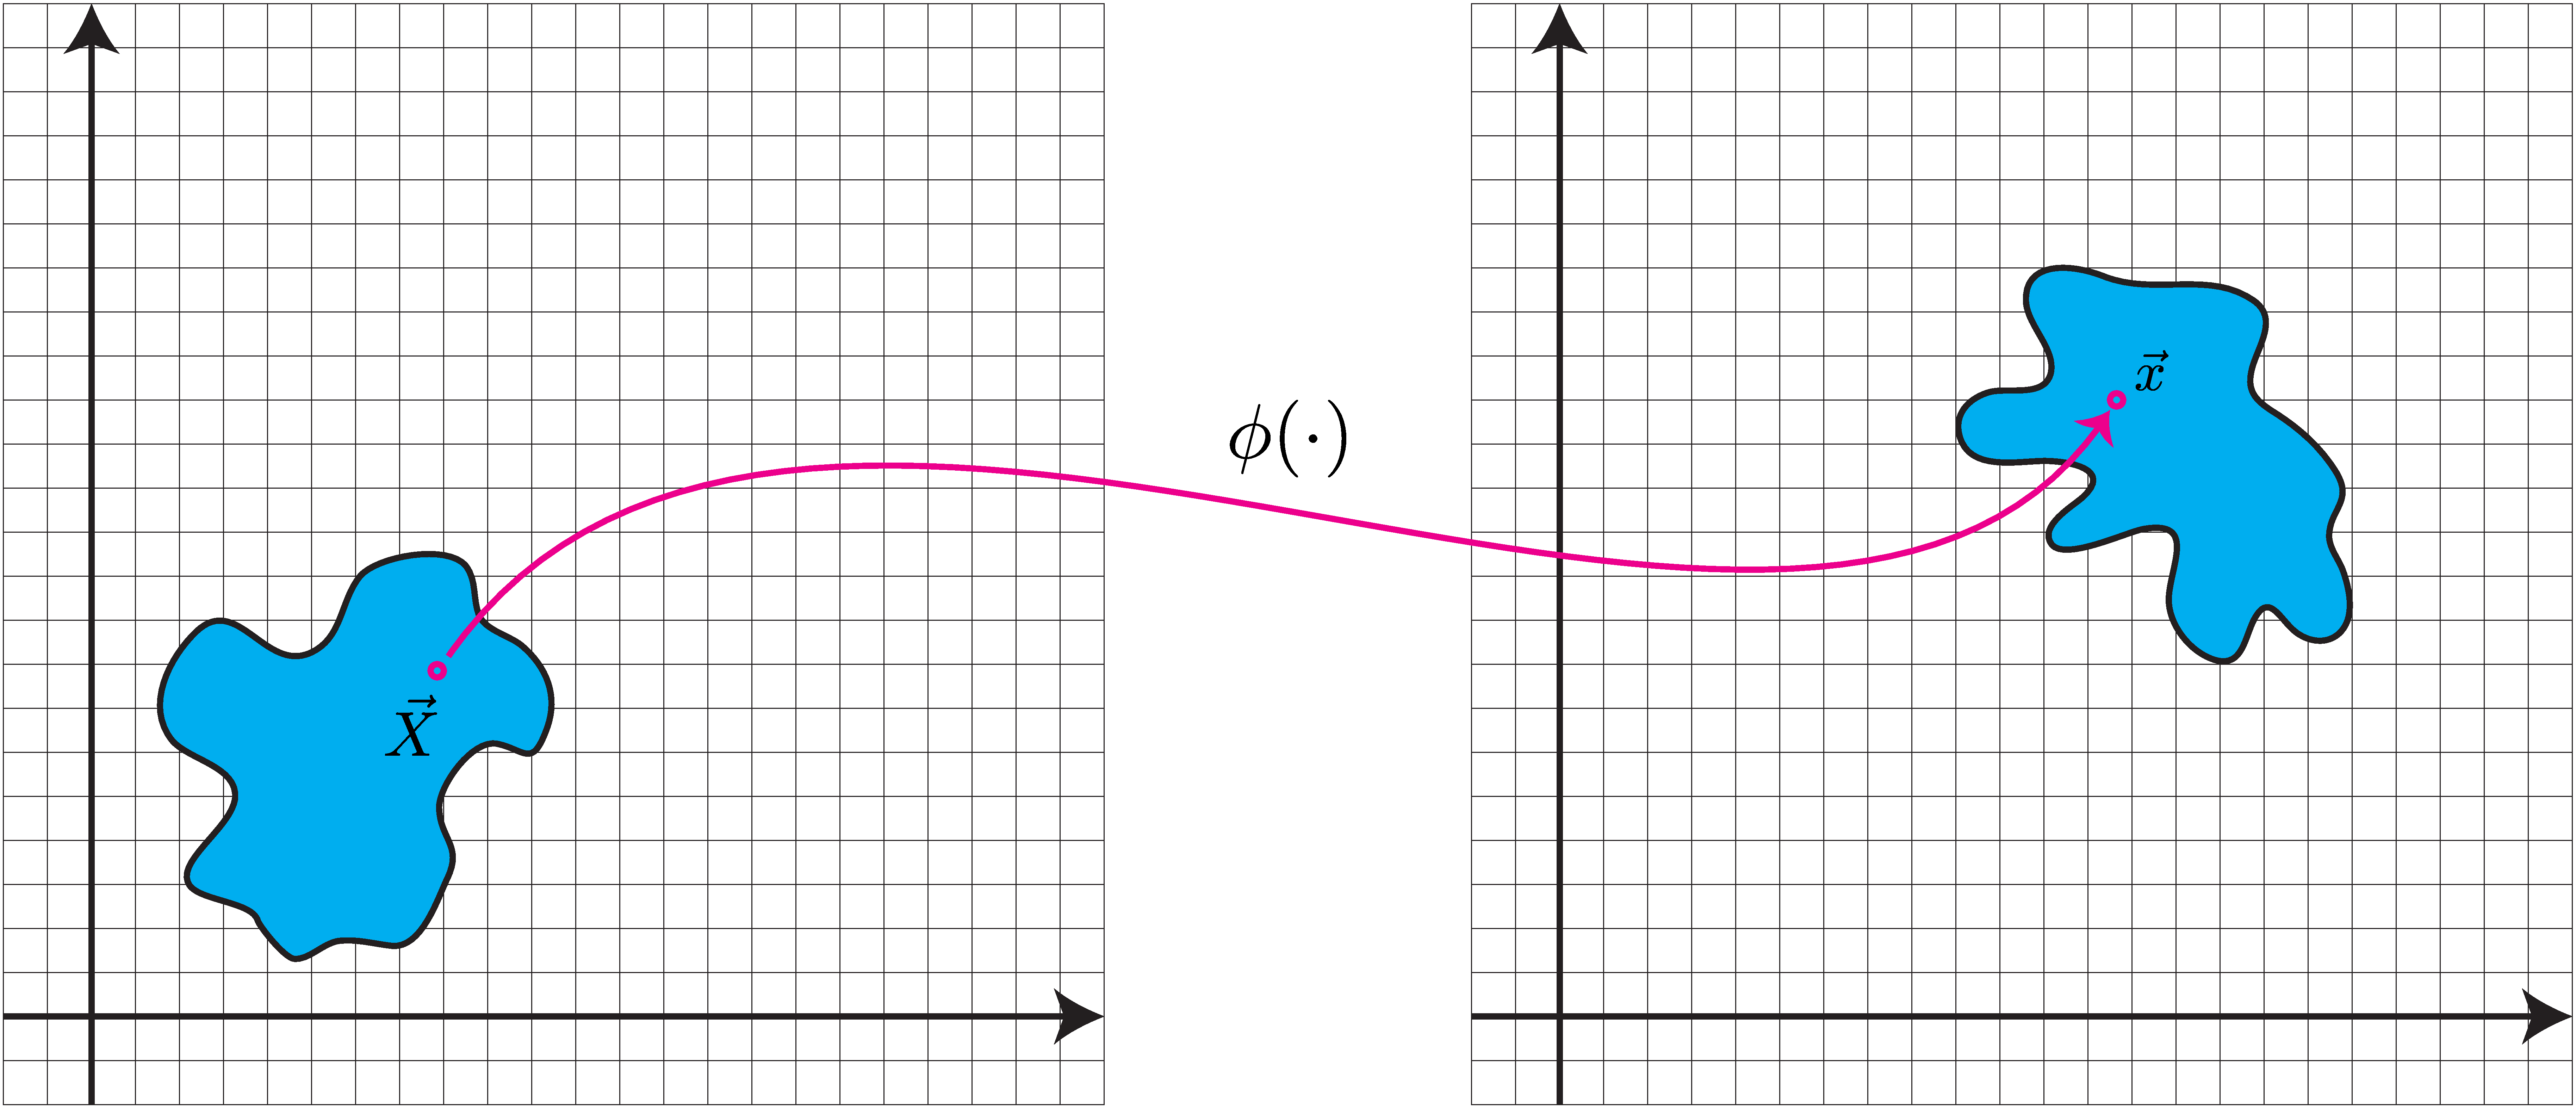
\includegraphics[width=\textwidth]{other_images/DeformationFigure.pdf}
  \vspace*{-.3in}
   \caption{Example Deformation Map}{The deformation map $\phi$ is
     illustrated here mapping between locations $\vec{X}$ in the
     object's reference configuration and corresponding deformed
     locations $\vec{x}$ in the object's deformed configuration.}
   \label{fig:deformationexample}
   \vspace*{-.15in}
\end{figure}

% If we recall Newton's Third Law of Motion, external forces applied to
% objects are met with an equal and opposite force. But if we look at
% the object fractionally, we would see that these opposing forces
% don't just exist on the surface, but are distributed internally
% throughout the object's material. These internal forces are referred
% to as mechanical stress. Stress is defined to be force applied over an
% cross-sectional area, or volume for three dimensional objects. If we
% were to look at a single point of an object, we could define the
% internal stress of that point by a second dimensional tensor, which
% describes what force vectors are felt by that point in three
% orthogonal directions. Ultimately, this internal stress field causes
% the object to deform, or change shape, resulting in strain - the
% mechanical term for a related tensor value which is defined as the
% ratio of changed length (or volume) compared to the original
% length (or volume). The strain tensor, in combination with the specific material
% being deformed, represents a quantity of potential energy. This energy
% represents the amount of work required to deform the object.  Given
% these basic mechanical deformation concepts, we can now develop a
% theoretical framework for simulating deformable objects.

% The first part of that process is describing our representation of
% state. To do so, we return to the object's shape. The deformation of
% an object is the change in shape between one configuration and
% another. In order to keep track of the deformation, we can record it
% relative to an object's reference configuration. This is an arbitrarily
% chosen shape in the coordinate system of the object from which all
% other deformations are measured. Mathematically, we can define the deformation as
% a mapping between the locations in the domain of the object and $\mathbf{R}^3$:
% $$\phi: \Omega \rightarrow \mathbf{R}^3$$. Under this regime, we
% consider the domain of $\phi$ to be points in $\Omega$, often referred
% to as material space locations as they can conceptually be considered
% infinitesimal blobs of undeformed material. We simultaneously locate and
% identify them by a spatial vector: $\vec{X} = (X, Y, Z)$. The points
% in $R^3$ which make up the image of $\phi$ are the corresponding
% deformed locations $\vec{x} = (x, y, z)$. It is worth noting that the reverse mapping
% could have been considered, i.e the mapping that projects from a shape
% back to the reference configuration. This type of relationship is
% not unusual in computer graphics, for instance via mesh
% parameterization for texture mapping. Unfortunately, this relationship
% is a little harder to deal with, especially if we wish to handle
% situations where the mapping is not one-to-one, such as when the
% deformation causes the object to overlap with itself. For the
% techniques presented in this document, we will be using a reference
% configuration that avoids self penetration and a forward deformation
% map to avoid these problems.

Now that we have defined for what it means for an object to be
deformed and the concept of a deformation map, we can return to the
relationship between shape, force, and energy. In order to relate
shape, or deformation, of an object to its energy, we need to define a
way to measure how the deformation varies throughout the object. We
facilitate this by defining the quantity called the deformation
gradient $\mathbf F$, the jacobian of the deformation map.

\begin{equation}
  \label{equ:deformationgradient}
  \mathbf{F}(\vec{X}) = \frac{\partial \phi(
      \vec{X} )}{ \vec{X} }
\end{equation}

From the deformation gradient, we can extract metrics of deformation,
known as strain measures. The strain measure is directly used to
compute the strain energy, the potential energy of the material due to
deformation. In the reference configuration, we want the
strain measure to be evaluate to zero. Additionally, if the object's
deformation is purely translational, we would also like the strain
measure to be zero. A simple strain measure that meets these goals
might be:

\begin{equation}
  \label{equ:simplestrainmeasure}
  s = \mathbf F - \mathbf I
\end{equation}

While this evaluates to zero under translation and no deformation,
this simple measure is non-zero under rotation, which can result in
inaccuracies under large deformation. We can treat this issue by
employing a different strain measure, the Green strain $\mathbf{E}$:

\begin{equation}
  \label{equ:greenstrain}
  \mathbf{E} = \frac 1 2 (\mathbf{F}^T\mathbf{F}-\mathbf{I})
\end{equation}

The Green strain is more robust to large deformations by virtue of it
being rotation invariant, but is non-linear and can behave
non-intuitively around extreme deformations. As an example, consider a
deformation that simply inverts an object along one axis. The Green
strain of this deformation would be zero in this case despite a
significant deformation. If we take a linear approximation around the
undeformed configuration of the Green strain, we arrive at the
\textit{small strain} $\epsilon$:

\begin{equation}
  \label{equ:smallstrain}
  \bm{\epsilon} = \frac 1 2 (\mathbf{F} + \mathbf{F}^T) - \mathbf{I}
\end{equation}

This formula is linear and under small deformations is approximate to
the Green strain, making it useful for scenarios with limited
deformation, such as structural simulations for buildings or other
near rigid objects. As the deformation increases however, the small
strain suffers from the similar problems as the simple strain
presented earlier (Equation \ref{equ:simplestrainmeasure}).  In order to get a strain measure that is
rotationally invariant and is more predictable than the Green strain,
one possibility is to apply a polar decomposition to the deformation
gradient in order to extract the rotational components:
\begin{equation}
  \label{equ:polarstrain}
  \begin{split}
    \mathbf F &= \mathbf R\mathbf S\\
    \bm \epsilon_c &= \mathbf S - \mathbf I
  \end{split}
\end{equation}
While this strain measure is still non-linear, it behaves similarly to
the small strain measure, including a linear (not quadratic)
relationship to axis aligned stretch, while maintaining rotational
invariance.

Once we have chosen our strain measure, we can use it to define a
strain energy density $\Psi(\mathbf{F})$. This is a measure of the
potential energy per unit volume of the material as a consequence of
undergoing deformation.  Similar to the strain measure, there are
several popular energy density functions which can describe generic
deformable materials. Linear elasticity (Equation
\ref{equ:linearelasticity}), derived from the small strain tensor, is
easy and uncomplicated to compute due to its linear relationship to
the deformation gradient. However, since it is based on the small
strain tensor, it is not rotationally invariant and can exhibit
physically inaccurate behaviors under large deformations.

\begin{equation}
  \label{equ:linearelasticity}
  \Psi(\mathbf{F}) = \mu \bm \epsilon : \bm \epsilon + \frac \lambda 2
  \text{tr}^2(\bm \epsilon)
\end{equation}

If we replace the strain measure used in the Linear
elasticity model with the Green strain, we get what is known as
the St. Venant-Kirchhoff energy density function (Equation
\ref{equ:stvenantkirchhoff}).
\begin{equation}
  \label{equ:stvenantkirchhoff}
  \Psi(\mathbf{F}) = \mu \mathbf{E} : \mathbf{E} + \frac \lambda 2
  \text{tr}^2(\mathbf E)
\end{equation}
While this model is more accurate under large deformations due to the
Green strain, it has the unfortunate property of not penalizing
significant compression and inversion. In the film production
industry, another nonlinear energy function is often used instead,
called Co-rotated elasticity, which is based off the fourth strain
measure detailed in Equation \ref{equ:polarstrain}:

\begin{equation}
  \label{equ:corotatedelasticity}
  \begin{split}
   \Psi(\mathbf{F}) &= \mu \bm \epsilon_c : \bm \epsilon_c + \frac \lambda 2
   \text{tr}^2(\epsilon_c)\\ &= \mu \lVert \bm S - \bm I \rVert^2_{\bm
     F} + \frac \lambda 2
   \text{tr}^2(S-I)
   \end{split}
\end{equation}

Finally, we can calculate the energy of the entire object by
integrating the energy density over the domain:

\begin{equation}
  \label{equ:systemenergy}
  E(\phi) = \int_\Omega \Psi( \mathbf F ) \,d\vec{X}
\end{equation}

In the next section, we will convert these continuous equations of
deformation and energy into discrete forms, allowing us to solve for
our object's deformations. Up until now, the equations we have been
using have assumed a continuous deformation field, free of any
particular discretization. The expressions in the next section will
replace these continuous equations with those appropriate for the
lattice based discretization we use in our application.

\section{Discrete form of Elastic Deformation}
\label{sec:engineering:solving}

With these equations in hand, we can now reason about how to produce
realistic mechanical responses from our virtual tissue models on a
computer. To do so, we need to change how we have been treating the
expressions from the previous section from a continuous representation
to a discrete representation suitable for computation. To do this, we
will be dividing our continuous domain in to smaller regions, or
elements. Each element represents a finite quanta of material, thus
giving rise to the name of the approach we will be using throughout
this document: Finite Element Method (FEM).

In our new discrete world, we must first translate our former
continuous domain $\Omega$ into a data structure representable on a
computer. Here we have a number of choices to pick from. FEM
literature has described many approaches for discretization over the
years, ranging from volumetric meshes to particle based
approaches. These designs can be evaluated over several categories:
regularity, conformity, and ease of use. Regularity refers to the
extent that the technique uses repeating data structures or provides
implicit internal relationships that can be predicted, which is often
extremely beneficial for performance optimization. Conformity refers
to how the data structure represents the object's boundary shape,
either attempting to directly replicate the object's domain or acting
as a scaffolding around it, which can affect the accuracy of the
simulation. Finally, ease of use is a catch all term that includes any
property which makes the data structure easy or troublesome to include
in higher level pipelines. In this document, the approach we will be
using is a mesh discretization. In particular, we will be using a
design referred to as an embedding lattice. Seen in Figure
\ref{fig:embeddingexample}, we have an example mesh of a lion and its embedding lattice. This data structure is extremely regular
and generally easy to construct, though it can suffer from a lack of
conformity.

\begin{figure}[t]
  \includegraphics[width=.5\textwidth]{other_images/LionStatue.png}
  \includegraphics[width=.5\textwidth]{other_images/LionLattice.png}
  \vspace*{-.3in}
   \caption{Lattice Embedding}{Show here is a three dimensional lion
     model\footnotemark (left) and the corresponding embedding lattice
     (right). Each vertex of the lion model is embedded into a cell of
   the lattice, which acts as a deformable scaffold around the model.}
   \label{fig:embeddingexample}
   \vspace*{-.15in}
\end{figure}

\footnotetext{The lion model was rendered with a shader created
  by Anthony Pilon.}

Under this representation, our material will be sampled at Cartesian
\textit{nodes} of a regular hexahedral lattice and our elements of computation
will be its \textit{cells}. We refer to these nodes as containing degrees of freedom, as
they represent the discrete points where deformation can occur. To
deal with the issue of conformity, we utilize a technique known as
lattice embedding - whereby the discrete boundary of our object,
represented by a separate surface mesh, is embedded in cells of the lattice
via a weighted interpolation of its nodes. Later in this document,
additional techniques will be presented to further increase the
accuracy of the lattice's boundary conformity. Since the
terms presented in regards to embedding can be confusing, we will
stick to the following terminology:

\begin{description}
\item[lattice] - The simulation lattice is the discrete representation
  of our simulation domain and is composed of elements of material known
  as cells. Through the simulation lattice, we compute deformation
  gradients, energy, and ultimately forces.
\item[node] - A node is a topological point in our simulation
  lattice. Each node is identified by a spatial location as a label
  and stores three degrees of freedom, or DOFs. These degrees of
  freedom are represented by the discrete deformation
  values. Additionally, nodes store the discrete forces resulting from
  this deformation.
\item[cell] - A cell is the basic computational unit of our simulation
  lattice. It is represented as a regular hexahedral volume and
  connects the eight nodes at its corners.
\item[mesh] - Our tissue material surface is represented by a mesh. This mesh
  is conforming, i.e it attempts to match the shape of the continuous
  domain as closely as possible. The deformed material surface is the
  desired visual result of our physical simulation.
\item[vertex] - A vertex is a topological point in our material
  mesh. Its position in space is wholly determined by its embedding
  relationship, typically bi-linear, to its parent cell in the
  deformation lattice.
\end{description}

Using this simulation lattice as a discrete approximation of our
continuous domain, we can now translate the concepts from the previous
section. Instead of material points, we have nodes. Each node is
labeled by an unique identifier. This identifier can be as simple as an
integer, e.g. Node 52, but since we are using a regular lattice, we
will continue with the previous spatial labeling, although in this case we
will now use integer coordinates. Our former concept of a reference
configuration will remain, by assigning each node a reference position
in space. Defining our deformation map $\phi$ then becomes as
simple as:
\begin{equation}
  \label{equ:discretedeformationmap}
  \phi(\vec{X};\mathbf x) = \sum_i x_i \mathcal N_i(\vec{X})
\end{equation}

We define $\mathbf x = {x_1, x_2, x_3, \ldots, x_n}$ to be our
discrete deformation state, which includes the displacement of every node in
our lattice from its reference location. In this expression
$\mathcal N_i$ is the \textit{shape function} for each node in the
cell. This shape function is used to interpolate the discrete nodal
displacements into a continuous deformation deformation field. For the
hexahedra we are using, our shape functions are derived from
trilinear interpolation. Using this
new description of $\phi$, we can derive a continuous definition of the
deformation gradient for any point $\vec{X}$ inside the cell just as
before:

\begin{equation}
  \label{equ:discretedeformationgradient}
  \mathbf F(\vec{X};\mathbf x) = \frac{ \partial \phi(\vec{X};\mathbf x)
  }{\partial \vec{X}}
\end{equation}

From this expression, we can integrate over the volume of a cell to
arrive at an expression for a cell's energy.:

\begin{equation}
  \label{equ:discreteenergy}
   E^e(\mathbf F) = \int_{\Omega_{e}}\Psi^e( \mathbf F(\vec{X};\mathbf x) ) \,d \vec{X}
\end{equation}

In order to evaluate the integral over the volume of the cell, we
employ a numerical quadrature approach. This discrete approximation of the
cell's energy is expressed in Equation \ref{equ:discreteenergyint}:

\begin{equation}
  \label{equ:discreteenergyint}
  \begin{split}
  E^e(\bm x) &= \int_{\Omega_{e}}\Psi^e( \mathbf F(\vec{X};\mathbf x) ) \,d \vec{X}\\
  &\approx ||\Omega_e||\sum^{\mathcal Q}w_q\Psi^e(\bm F(\vec{X}_q;\bm
  x)) = \hat{E}^e(\bm x)
  \end{split}
\end{equation}



Here, we are evaluating $\mathcal Q = \{\vec{X}_1,\vec{X}_2,...,\vec{X}_q\}$
quadrature points, each with a individual weight $w_q$, such that
$\sum_q w_q = 1$. $||\Omega_e||$ corresponds to the volume of an
individual cell. Our choice of quadrature points greatly affects the
accuracy of the approximation. Using an eight point Gauss quadrature,
while expensive, is third-order accurate for regular, axis-aligned hexahedra. For more
accuracy at cells which are only partially covered with material,
\cite{PatteMS:2012} demonstrated an alternative quadrature scheme that
second order accurate and uses four points. Finally, one point quadrature is possible
\citep{McAdaZSETTS:2011} if an additional stabilization energy term is
included to compensate for unpenalized deformation modes.

At this point, it is straightforward to define the global discrete
energy to be the sum of every cell's energy:

\begin{equation}
  E(\mathbf x) = \sum_e \hat{E}^{e} 
\end{equation}

From these expressions, we can derive an expression for forces at each
node by simply taking the derivative of the systems energy at each
cell and summing its contribution onto the node:
\begin{equation}
  \label{equ:discreteforces}
  \vec{f}_i(\mathbf x) = \sum_{e} \vec{f}_i^{\;(e)}(\mathbf x)
  \text{, where } \vec{f}_i^{(e)} = - \frac{\partial \hat{E}^{e}(\mathbf x)}{\partial x_i}
\end{equation}

We define $\mathbf f = {\vec{f}_1, \vec{f}_2, \vec{f}_3, \ldots, \vec{f}_n}$ as
our force state, which is similar to our deformation state $\mathbf x$.
Using this relationship between nodal displacements and nodal forces,
we can finally describe the process for computing deformations.

%For the purposes of this discussion, we'll be limiting our focus to
%quasi-static deformation simulation sequences. Quasi-static deformations are the
%result of the system being solved for internal equilibrium after we
%change external positioning constraints and boundary conditions.

\subsection{Solving for Deformations}

When a real object is exposed to external forces and constraints, it
will naturally attempt to assume a shape that equilibrates its
internal energy with its external constraints. We will seek the same
situation in our case by solving for a deformation which corresponds
to a local minimum in the object's energy $E$. This is equivalent to
solving for a deformation state $\mathbf{x}$ such that
$\mathbf{f}(\mathbf{x}) = 0$, as minimums in $E$ correspond to zero
values in its first derivative, i.e. the discrete force state
$\mathbf{f}$.

Since the relationship between forces and deformation is generally
non-linear, unless we use the linear elasticity model for small
deformation situations, we employ the standard Newton-Rhapson method
to determine the solution. This method uses a series of linear
approximations to determine the roots of our function $\mathbf
f(\mathbf x)$. Given some initial configuration
$\mathbf x_0$, which will typically be the last equilibrium shape, our
goal is to find a $\delta \mathbf x$ such that $\mathbf f(\mathbf x_0 + \delta \mathbf
x) = 0$. To solve for $\delta \mathbf x$, consider the Taylor
expansion of this expression:
\begin{equation}
  \label{equ:newtontaylor}
  \begin{split}
    \mathbf f(\mathbf x_0 + \delta \mathbf x) &= \mathbf f(\mathbf x_0) + \frac{ \partial \mathbf f }{\partial \mathbf x}
    \delta \mathbf x + O(\delta \mathbf x^2)\\
    \mathbf f(\mathbf x_0 + \delta \mathbf x) &\approx \mathbf f(\mathbf x_0) + \frac{ \partial \mathbf f }{\partial \mathbf x}
    \delta \mathbf x\\
  \end{split}
\end{equation}
If we assume that $\mathbf f(\mathbf x_0 + \delta \mathbf x) = 0$, since this is our goal, we
can solve for an approximate solution to $\delta \mathbf x$:
\begin{equation}
  \label{equ:newtonupdateder}
  \begin{split}
    0 &\approx \mathbf f(\mathbf x_0) + \frac{ \partial \mathbf f }{\partial \mathbf x}
    \delta \mathbf x\\
    -\frac{ \partial \mathbf f }{\partial \mathbf x} \delta \mathbf x &\approx \mathbf f(\mathbf x_0)\\
    \delta \mathbf x &\approx (-\frac{ \partial \mathbf f }{\partial \mathbf x}^{-1})\mathbf f(\mathbf x_0)
  \end{split}
\end{equation}
Which suggests an update formula for $x$:
\begin{equation}
  \label{equ:newtonupdate}
  \mathbf x_{n+1} = \mathbf x_n - \bigg(\underbrace{-\frac{ \partial \mathbf f }{\partial
      \mathbf x}\bigg\rvert_{\mathbf x_n}}_{\mathbf K(\mathbf x_n)}\bigg)^{-1}\mathbf f(\mathbf x_n)
\end{equation}

We refer to the matrix $\mathbf K$ as the \textit{stiffness
  matrix}. In order to arrive at a solved equilibrium configuration, for
each iteration $n$ our task becomes the following steps:

\begin{enumerate}
  \item Update the stiffness matrix $\mathbf K$ for the current
    configuration $\mathbf x_n$.
  \item Compute forces $\mathbf f_n$ corresponding to $\mathbf x_n$
    for our right hand side of the update expression.
  \item Terminate if we are within tolerance to zero net forces.
  \item Solve $\mathbf K^{-1}$ for a displacement update $\delta \mathbf x$.
  \item Update our current deformation state $\mathbf x_{n+1} = \mathbf x_n +
    \delta \mathbf x$
  \item Repeat
\end{enumerate}

At the end of this process, our final deformation shape will be the
one that equilibrates the internal and external forces of the
object. We can use this process to create animations by solving for a
series of \textit{quasi-static} poses. These poses are controlled by
time varying constraints which are successively applied to the object
between solves. If moved in smooth trajectories, these constraints can
create the appearance of smooth deformation, despite the simulation
converging to a static pose at every iteration. This can be thought of
as taking snapshots of an object's motion, similar to how film is
captured, though it does not include dynamic effects such as jiggling
or damped motion. However, this approach is much more robust and can
handle rather sudden and dramatic departures from prior constraints
more readily than techniques that allow more dynamic motions.
  
Unfortunately, the solution to $\mathbf K^{-1}$ is not without
significant challenges. Some of the major difficulties include:
\begin{description}
\item [Memory Footprint] Each entry in $\mathbf K$ is a relation
  between force along one axis and displacement along another between
  every connected degrees of freedom. Quantitatively, this means we
  are faced with a matrix which has 27 non-zero entries on each row,
  where each entry is a dense three by three matrix. To simply store
  $\mathbf K$ for a modest sized domain of $128^3$ degrees of freedom,
  it would require 500 million scalar values at just under two
  gigabytes of storage if 32-bit floating point representation is
  used\footnote{This is not including any additional storage cost
    overheads for representing the sparse matrix itself. This number
    is simply the space required to store only the non-zero
    coefficients alone.}. Since we are required to rebuild and then
  solve this matrix repeatedly, this footprint represents a
  significant bottleneck on most platforms where available compute
  bandwidth exceeds memory bandwidth by an order of magnitude.

  \item [Solver Choice] Since our goal is to solve a large linear
    system, we have several options including both direct and
    iterative style solvers. However, both general techniques have
    different and significant drawbacks. Direct solvers are generally
    robust even when the matrix is poorly conditioned due to stiff
    constraints or non-uniform materials. Unfortunately, direct
    solvers typically work via a factorization and backward
    substitution solution, which both requires storing the entire
    matrix and then performing relatively little computation over its
    entries compared to the memory reads, making their performance
    poor on very large systems. Iterative solutions in contrast can do
    away with storing the entire matrix, instead only requiring that its
    multiplicative effect can be provided. This approach is known as
    a \textit{matrix-free} solution. Iterative methods are potentially faster
    and allow early termination for approximate solutions, but they
    are sensitive to matrix conditioning. Iterative solvers can also
    be slow to propagate effects throughout the domain, focusing on
    local errors before global smoothness.

  \item[Performance Concerns] When computing the solution to
    $\mathbf K^{-1}$, attention needs to be paid to how
    parallelization through multithreading and vectorization can be
    used to increase performance. What makes this task particularly
    tricky is that by being more efficient with computation only makes
    the divide between available memory and computation bandwidth even
    worse. Careful management of access patterns and data organization
    needs to be done in order to avoid starving the processor and
    undoing any advantage parallelization can bring. An additional
    concern is that if explicit construction of $\bm K$ is required,
    considerable expense must be paid for building a data structure
    used for a single Newton step. We can avoid this issue by sticking
    with solutions which don't require explicit construction.
 
\end{description}


\subsection{Discrete Formulas}
\label{sec:engineering:discreteformulas}

\afterpage{
\begin{algorithm}[p]
  \begin{minipage}{1\textwidth}
    %\begin{subalgorithm}{\textwidth}
      \setlength{\baselineskip}{1.35em}
      \begin{algorithmic}[1]
        \vspace{.2in}\Procedure{FElastic}{$\mathbf x^e$, $\mathcal Q$, params $p$}
        \State \Reshape $\mathbf x^e \rightarrow\mathbf{D}_s$
        \For{$q \in \mathcal Q$}
        \State \Compute $\mathbf G \leftarrow \Call{Gradient}{X_q}$
        \State \Compute $\mathbf{F} \leftarrow \mathbf{D}_s\mathbf{G}^T$
        \State \Compute $\mathbf P \leftarrow \Call{P}{\mathbf F, p}$
        \State \Accum $\mathbf{H} \leftarrow
        \frac{V_0}{w_q}\mathbf{PG}$
        \EndFor
        \State \Reshape \& \Accum $\mathbf{H} \rightarrow \mathbf{f^e}$
        \EndProcedure\vspace{.4in}
      \end{algorithmic}
    %\end{subalgorithm}
    \end{minipage}
    
  \begin{minipage}{1\textwidth}
    %\begin{subalgorithm}{\textwidth}
      \setlength{\baselineskip}{1.35em}
      \begin{algorithmic}[1]
        \Procedure{$\delta$FElastic}{$\delta \mathbf x^e$,$
          \mathbf x^e$,$\mathcal Q$, params $p$} 
        \State \Reshape $\mathbf x^e \rightarrow \mathbf{D}_s$,
        $\delta{} \mathbf x^e \rightarrow \delta{} \mathbf{D}_s$
        \For{$q \in \mathcal Q$}
        \State \Compute $\mathbf G \leftarrow \Call{Gradient}{X_q}$
        \State \Compute $\mathbf{F} \leftarrow
          \mathbf{D}_s\mathbf{G}^T$, $\delta{} \mathbf{F} \leftarrow
        \delta{} \mathbf{D}_s\mathbf{G}^T$
        \State \Compute $\mathcal{T} \leftarrow
          \Call{dPdF}{\mathbf F, p}$
        \State \Compute $\delta\mathbf{P} \leftarrow \mathcal T :
        \delta \mathbf F$
        \State \Accum $\delta{}\mathbf{H} \leftarrow
        \frac{V_0}{w_q}\delta{}\mathbf{PG}$
        \EndFor
        \State \Reshape \& \Accum $\delta{}\mathbf{H} \rightarrow
        \delta{}\mathbf f^e$
        \EndProcedure
      \end{algorithmic}
    %\end{subalgorithm}
    \end{minipage}
    \vspace{.15in}
  \caption{Algorithm for computing elemental elastic force and force
    differentials}{These two algorithms for elemental forces and force
    differentials, respectively, receive as input values from each of
    the eight nodes of a cell $e$, indicated by $x^e$, and accumulate
    forces back onto these nodes. The functions \textsc{P} and \textsc{dPdF}
    can be user-defined to implement arbitrary isotropic
    materials, controlled by material parameters $p$. The
    \textbf{reshape} operation concatenates eight nodal vectors in a
    cell (positions, forces, etc) into a $3\times 8$
    matrix and vice versa. $\mathcal Q$ is the set of quadrature points
    used to approximate the volume integral. $\mathbf{G}$ is a
    $3\times 8$ gradient matrix encoding the derivative of the shape
    functions. $V_0=h^3$ is the volume of the
    cartesian cell. $\mathcal{T}$ is a sparse 4th order tensor as
    defined in \protect\cite{TeranSIF:2005} }
  \label{alg:isotropicforces}
\end{algorithm}
\clearpage
}

In order to invert $\bm K$ without forming an explicit copy of the
matrix, we can use algorithms which are referred to as matrix-free,
such as Conjugate Gradients (CG). These techniques operate by taking
products of the form $\bm K(\bm x_n) \delta \bm x$, where $\delta \bm
x$ is an arbitrary vector used by the specific algorithm being
employed (for convenience, we label this vector as $\delta \bm x$,
though it does not necessarily correspond to a deformation or
displacement).
\begin{equation}
  \bm K(\bm x_n) \delta \bm x = -\bigg(\frac{\delta \bm f}{\delta \bm
    x}\bigg|_{\bm x_n}\bigg)\delta \bm x
\end{equation}
The product of $(\frac{\delta \bm f}{\delta \bm
    x}|_{\bm x_n})\delta \bm x$ is  equivalent to the
  \textit{differential} $\;\delta \bm f [ \delta \bm x; \bm x_n ] = (\frac{\delta \bm f}{\delta \bm
    x}|_{\bm x_n})\delta \bm x$. In this section, we'll cover the
  process of computing discrete values for this differential, along
  with the corresponding forces (the right
  hand side of Equations
  [\ref{equ:newtonupdateder},\ref{equ:newtonupdate}] ).


\paragraph{Trilinear elements and gradients} We start by deriving a
concise expression for the deformation gradient
$\mathbf{F}(\vec{\mathbf X};\bvec{\mathbf x})$. We use the notation
$\{\vec{\mathbf X}_{i_1i_2i_3}\}\;\text{s.t.}\;\{i_1,i_2,i_3\}\in\{0,1\}$ for the eight
vertices of a given cell with
$\vec{\mathbf X}_{i_1i_2i_3}=\vec{\mathbf X}_0+(i_1,i_2,i_3)h$,
where $h$ is the diameter of a cell. Their
respective interpolation basis functions are
$\mathcal{N}_{i_1i_2i_3}(\vec{\mathbf X})=\prod_k(\xi_k)^{i_k}(1-\xi_k)^{1-i_k}$
where
\begin{equation*}
  \begin{aligned}
\vec{\xi}(\vec{\mathbf
  X})&=(\xi_1,\xi_2,\xi_3)\\
&=(X-X_0,Y-Y_0,Z-Z_0)/h
\end{aligned}
\end{equation*}
are the trilinear coordinates of $\vec{\mathbf X}$. Partial derivatives of the
interpolating functions are readily computed as
$\partial_j\mathcal{N}_{i_1i_2i_3}(\vec{\mathbf X})=(-1)^{1-i_j}\prod_{k\ne
  j}(\xi_k)^{i_k}(1-\xi_k)^{1-i_k}$.
From this point, we shall refer to the vertices of a specific cell
simply as $\vec{\mathbf X}_1...\ \vec{\mathbf X}_8$, and
$\mathcal{N}_1(\vec{\mathbf X})...\ \mathcal{N}_8(\vec{\mathbf X})$ for the
respective trilinear basis functions, with the understanding that we
know how to relate to the prior indexing convention.  By equations
(\ref{equ:discretedeformationmap},\ref{equ:discretedeformationgradient}) the
deformation gradient at a location $\vec{\mathbf X}_\ast$ is
\begin{equation}
  \label{equ:discretef}
  \begin{aligned}
    \mathbf F(\vec{\mathbf X}_\ast;\mathbf x) &=
    \sum_i\vec{\mathbf x}_i\nabla\mathcal{N}_i(\vec{\mathbf
      X}_\ast)^T\\
    &=\mathbf{D_s}(\bvec{\mathbf x})\mathbf{G}(\vec{\mathbf X}_\ast)^T\\
  \end{aligned}
\end{equation}
where
$\mathbf{D_s}(\bvec{\mathbf x})=\left[\vec{x}_1\ \vec{x}_2\ \hdots\
  \vec{x}_8\right]\in\mathbf{R}^{3\times 8}$
is the cell shape matrix. The matrix
$\mathbf{G}(\vec{\mathbf X}_\ast)\in\mathbf{R}^{3\times 8}$ with
$\mathbf G_{ij}(\vec{\mathbf X}_\ast)=\partial_i\mathcal{N}_j(\vec{\mathbf X}_\ast)$ will be
referred to as the gradient matrix at $\vec{\mathbf X}_\ast$. Note that for
any material point $\vec{\mathbf X}_\ast$, $\mathbf{G}(\vec{\mathbf X}_\ast)$ can be
precomputed as its value is independent of any deformation.
\vspace*{-.1in}
\paragraph{Force computation} We mimic the elastic force derivation
from \cite{McAdaZSETTS:2011},
referring to Equations [\ref{equ:discreteenergyint},\ref{equ:discreteforces}], for an individual force components
$f_i^{(j)}$, where $i$ indicates which node and $j \in \{1,2,3\}$
indicates the axis:

\begin{equation}
  \begin{split}
    f_i^{(j)} &= -\frac{\partial E^e}{\partial x^{(j)}_i} =
    -h^3\frac{\partial \Psi(\bm F^e) }{\partial x^{(j)}_i} \\ &=
    -h^3\sum_{k,l}\frac{\partial \Psi(\bm F^e) }{\partial F_{kl}}\bigg|_{\bm F^e}
    \frac{\partial F^e_{kl} }{\partial x^{(j)}_i} \\
    & = -h^3\sum_{k,l}[\bm P(\bm F^e)]_{kl}G^e_{li}\delta_{ik}\\ &=
    -h^3\sum_{l}[\bm P(\bm F^e)]_{jl}G^e_{li}
  \end{split}
\end{equation}


Continuing from this expression, we can pack, or \textit{reshape}, the
resulting forces into a unified matrix:
$\mathbf{H}_e(\bvec{\mathbf x})=[\vec{f}_1\ \vec{f}_2\ \hdots\
\vec{f}_8]$, which is a $3\times 8$ matrix containing all nodal elastic forces in a
cell $\Omega_e$. The force matrix $\mathbf{H}_e$, for a set of
quadrature points $\mathcal Q$, is assembled as:
\begin{equation}
\mathbf{H}_e(\bvec{\mathbf x})=-h^3 \sum_{\mathcal Q} w_q\mathbf{P}(\mathbf{F}(\vec{\mathbf X}_q;\bvec{\mathbf x}))\mathbf{G}(\vec{\mathbf X}_q)
\end{equation}
$$
\mbox{where}\ \
\mbox{$\mathbf{P}(\mathbf{F})=\partial\Psi(\mathbf{F})/\partial\mathbf{F}$}.
$$
In this last expression, $\mathbf{P}$ is the 1st
Piola-Kirchhoff stress tensor.

\paragraph{Force differentials} The Conjugate Gradients (CG) solver
used to solve equation (\ref{equ:newtonupdateder}) does not require
the matrix $\mathbf{K}(\bvec{\mathbf x}_n)$ to be explicitly
constructed, as long as its action on an input vector
$\delta\bvec{\mathbf x}$ can be evaluated.  The result of this
implicit matrix-vector multiplication are the force differentials
$\delta\bvec{\mathbf f}$. We perform this matrix-free operation on an
element-by-element basis, adding the contribution of each $\Omega_e$
to the aggregate differentials.  The force differentials can
be collectively computed as
$\delta\mathbf{H}_e(\delta\bvec{\mathbf x};\bvec{\mathbf x})=[\delta\vec{f}_1\ \delta\vec{f}_2\ \hdots\
\delta\vec{f}_8]$, described in \cite{McAdaZSETTS:2011} and \cite{PatteMS:2012}, as
follows:
%% \vspace*{-.15in}
\begin{equation}
\delta\mathbf{H}_e(\delta\bvec{\mathbf x};\bvec{\mathbf
    x})=-h^3\sum_{\mathcal Q} w_q\delta\mathbf{P}(\delta\mathbf{F};\mathbf{F}(\vec{\mathbf
    X}_q;\bvec{\mathbf x}))\mathbf{G}(\vec{\mathbf X}_q)
\end{equation}
$$
\mbox{where}\ \ \mbox{$\delta\mathbf{P}(\delta\mathbf{F};\mathbf{F})=\mathcal{T}(\mathbf{F}):\delta\mathbf{F}$},
$$
$$
\mbox{and}\ \
\mbox{$\delta\mathbf{F}=\mathbf{D_s}(\delta\bvec{\mathbf
    x})\mathbf{G}(\vec{\mathbf X}_q)^T$}.
$$
%% \vspace*{-.15in}
In this expression, the fourth order tensor
$\mathcal{T}=\partial^2\Psi/\partial\mathbf{F}^2$ is the stress
derivative. We refer the reader to \cite{TeranSIF:2005} for a
discussion of how this tensor can be constructed via the SVD for
isotropic materials.


% Also, note that due to our use of the defect
% correction iteration, only a single quadrature point (the cell center
% $\vec{X}_c$) was used in the equations above.
% \paragraph{Definiteness fix} A number of authors
% \cite{TeranSIF:2005,McAdaZSETTS:2011} have emphasized the necessity to
% address the possible indefiniteness of the stiffness matrix
% $\partial\bvec{f}/\partial\bvec{x}$ for nonlinear materials. In our
% case, since we do not employ Conjugate Gradients as these methods do,
% the definiteness of the stiffness matrix is not a strict
% requirement. However, we observed that, in the absence of such
% modification, the Newton-Raphson procedure would sometimes converge to
% local minima, or even unstable force equilibrium configurations, which
% were seen as perfectly acceptable saddle points by our QMR
% algorithm. This issue was alleviated by performing a version of
% definiteness fix similar to the previously mentioned approaches. In
% particular, if we consider the original energy definition
% $E(\bvec{x},\mu,\kappa)$ (prior to the introduction of pressures), the
% stiffness matrix is defined as
% $\mathbf{K}_{\mu,\kappa}=-\partial^2E(\bvec{x},\mu,\kappa)/\partial\bvec{x}^2$,
% where we explicitly included a reference to two (representative)
% material parameters $\mu$, and $\kappa$. Following the methodology of
% \cite{TeranSIF:2005}, we compute a modified stiffness matrix
% $\mathbf{\hat{K}}_{\mu,\kappa}$ by projecting $\mathbf{K}$ to its
% positive definite part. However, in order to avoid problematic
% conditioning, in case this positive definite correction has added a
% term proportional to the (very high in incompressible materials)
% parameter $\kappa$, we compute the following correction instead:
% $$
% \mathbf{K}_{\mbox{\small corr}}=\mathbf{\hat{K}}_{\mu,\kappa^\ast}-\mathbf{K}_{\mu,\kappa^\ast}
% $$
% where $\kappa^\ast$ is a thresholded value of the incompressibility
% penalty, corresponding to a Poisson's ratio in the range of
% $\nu\approx 0.3-0.4$. Subsequently, we add the correction term
% $\mathbf{K}_{\mbox{\small corr}}$ to the top-left block of matrix
% $\mathbf{K(u}_k\mathbf{)}$ in equation (\ref{eqn:newton-raphson}). We
% observed excellent performance with this adjustment, which was fully
% adequate for all our academic and biomechanics examples. Similar to
% the defect correction procedure, this modification does not affect the
% computed solution, only changes the iterative procedure that converges
% to it.




  \section{Constraints}

  Until this point, the discussion of materials and mechanical
  responses has not mentioned the last component of the initial
  problem statement: constraints. This is a complex
  topic and it is best to approach it after having a basic
  understanding of how simulated materials are solved in general. At
  basic level, a constraint is a condition we are either forcing or
  strongly encouraging the simulation to meet. For our purposes, we
  will consider two general categories of constraints, defined by
  their use cases: animated user interaction constraints and static
  scene constraints. 

  \subsection{User Interactions}
  
  User interaction constraints are the mechanism through which users
  are able to control and direct the simulation. In the real world, we
  interact with objects intuitively - we push and pull things, glue
  them in place, or join them via mechanical connectors. For simulated
  objects, we can perform many of the same conceptual tasks by mapping
  their high level descriptions into the fundamental forces behind
  them. Our benchmark application will support two primary types of user
  interaction constraints: hook constraints and suture constraints.  

  A hook constraint acts to pull material locations towards user
  specified points in space. This constraint is treated as an
  influence, not a hard requirement. During the simulation, a user is allowed
  to place an arbitrary number of hooks, move their target locations,
  and remove them. We consider these hooks to be animated, as the user
  is allowed to dynamically alter them over the course of the
  simulation. However, as was discussed before, our simulation is
  quasi-static - meaning that changes to the hooks can only occur
  in between solve steps. While this prevents a user from having
  smooth control, we can create its illusion by decreasing the time of
  each solve step. In later Chapters we'll look at techniques for
  improving raw performance, but we can also stop the Newton method
  early - displaying partially converged deformations to the user, but
  allowing them the opportunity to engage in further control actions
  to refine the partial results.

  Suture constraints are similar to hook constraints, in that they
  pull material towards other locations, except sutures pull two
  material locations towards one another instead of arbitrary spatial
  locations. Users are allowed to place and remove sutures during the
  simulation, just like hook constraints. However, they are not
  allowed to move them. Once created, a suture acts as a
  semi-permanent influence between two material locations, attempting
  to pull them together.

  Both hooks and sutures are allowed to be placed in arbitrary
  material locations and are not restricted to discrete locations,
  like nodes. This is accomplished by embedding them, similar to how
  we embed vertices of the surface mesh. However, in this case we are
  embedding a constraint point which imparts external forces on its
  embedding cell, rather than the cell imparting a deformation on the
  point, as would be the case for a vertex. To generate these forces,
  we implement hooks and sutures as as zero-rest length springs, which obey
  the simple one dimensional form of Hooke's law:
  \begin{equation}
    \label{equ:hookeslaw}
    \vec{f} = -k\lVert x_a - x_b\rVert_2
  \end{equation}
  In this relationship, the restorative forces (forces acting in a
  direction to return the spring to its resting length) $\vec f$ are
  proportional to the amount the spring has been stretched,
  represented by the distance between its two end points $x_a$ and
  $x_b$, all of which is modulated by a spring constant $k$. In our
  case, the endpoints $x_a$ and $x_b$ might be absolute positions, or
  they may be relative to a cell, defined by a set of trilinear
  interpolation weights. The forces, similarly, are applied by
  distributing themselves to their surrounding nodes through the
  inverse of the interpolation operation.

  \paragraph{Challenges} In terms of the equations we've looked at before, force constraints
  modify both the stiffness matrix $\bm K$ and the right-hand side
  $\mathbf f$ in Equation \ref{equ:newtonupdate}. This immediately
  suggests several technical challenges. First, there is a question of
  the strength of the spring constant $k$. This value directly
  controls how much influence the constraint exerts on the material to
  which it is attached. If it is made too weak, the hooks and sutures
  will not look realistic, not moving the material enough. If there
  are too many springs embedded in a cell, there may be insufficient
  degrees of freedom available to satisfy the constraints, creating
  locking behaviors. Strong springs can also cause iterative methods
  like CG to spend large amounts of effort correcting their local
  effects, leading to slow global convergence.  Hooks and sutures
  additionally disrupt the regularity aspects of the deformation
  lattice, making the force computations in some cells different from
  others. Sutures are more challenging, as they additionally introduce
  non-local effects - forces in one cell depend on the deformation of
  a potentially far away cell, instead of its immediate neighbors.
  
  \subsection{Scene Constraints}

  The second category of constraints are the static scene
  constraints. In this case static is referring to the notion that the
  user does not have control over the creation of these constraints
  and that they are instead initialized once for each surgical
  model. This is a subtle distinction, which will be more clear during
  the discussion about collision handling a little later. There are
  two types of scene constraints that are employed in our application:
  positional constraints and contact constraints. 

  Arguably the easiest constraint type, positional constraints can be
  thought of as holding a part of an object fixed in space with
  infinitely strong glue. Mathematically speaking, these constraints
  are referred to as \textit{Dirichlet}, or boundary conditions which
  are defined by enforcing a specific value at a
  location. Numerically, Dirichlet conditions are applied by enforcing
  a specific deformation on constrained nodes, usually being no
  deformation. For virtual surgery, these constraints could serve to
  pin the edges of tissue down, or act as a transition between the
  simulated and non-simulated regions, preventing separation. For our
  application, we enforce positional constraints only at node
  granularity as this is relatively easy and satisfies the use cases
  we have.

  Contact handling, or collision handling, is the constraint which
  exists to prevent one object from non-physically penetrating another
  object. Collision is a particularly tricky property to support in
  elastic simulation, especially self collision. Collision can be
  broken into two distinct steps: collision detection and collision
  response. \textit{Collision detection} is the aptly named process of
  determining whether or not collision has occurred at any particular
  point in time. For volumetric objects, which possess distinct inside
  and outside regions, collision detection typically takes the form of
  testing for surface penetration. This task, in a general sense, is
  rather expensive, so we reduce the computational load by restricting
  our tests to specific locations, or proxies. Proxies are points
  distributed (and embedded into the simulation lattice) over the
  surface of the object, creating a discrete stand-in for the true
  surface. The next step is determining which proxies are currently in
  states of collision or interpenetration.

  For rigid body collisions, i.e. collisions between the soft body and
  an external rigid object, level sets have been employed quite
  successfully for collision detection
  purposes\citep{TeranSIF:2005,McAdaZSETTS:2011} with complexities in
  the order $O(1)$ for any point of interest. The general idea is to
  define a level set over a rigid body and then between each
  quasi-static solution check which proxies are in a state of
  penetration. For each proxy that is colliding, the \textit{collision
    response} we employ is a penalty force. This takes the form of an
  additional spring constraint we introduce between the proxy and the
  closest location on the surface of the object, which can be
  determined via the level set. This spring, over the course of
  subsequent solves, acts to push (or pull) the material into a
  non-colliding state.  Self collision scenarios work similarly, but
  with an additional complication that both surfaces involved are
  potentially deforming. This topic will be covered in more detail in
  Chapter \ref{chp:nonmanifold}, where a full collision processing
  algorithm with level sets will be described.

  \paragraph{Challenges} The primary difficulties with this approach
  are due to geometry, robustness, and performance. The first problem
  that comes up is that our proxies need to be a good representation
  of our object's surface. Too few and we can miss substantial
  penetrations. But too many can be needlessly expensive to handle
  during the collision response phase. Distribution is important as
  well. For instance, choosing to place a proxy at the barycenter of
  each embedded mesh triangle is only reasonable if the mesh is
  uniformly discretized - uneven coverage of large and small triangles
  can lead to uneven collision detection. Additionally, since our
  penalty forces are implemented via spring constraints, we suffer
  from the same robustness issues discussed earlier for user
  constraints. Only now we have many more such constraints,
  potentially orders of magnitude more, making the problem more
  delicate. This approach can also suffer from instabilities relating
  to the discrete nature of the penalty forces - as proxies return to
  non-colliding states, other forces acting on the object can easily
  push them back, creating a pseudo-vibratory behavior as penalty
  forces are removed and reinstated.  Finally, we need a way of
  handling the response in a performant manner. Before we mentioned
  that springs can break the regularity of the stiffness matrix making
  parallelization more difficult, but now we have lots of springs
  which only intensifies the potential problems.  Maintaining reasonable
  performance in the face of these challenges will be touched on in
  Chapter \ref{chp:parallelization}.

\section{Topology Change}

  The last topic that needs to be discussed in relation to simulation
  and constraints is the concept of topology change. Apart from physically
  moving tissue around or joining it with sutures, this interaction
  represents a user's ability to incise material with some type of
  virtual cutting implement. As such, supporting topology change is very
  important as without support most surgical procedures would be impossible to
  perform. It is worth considering the ways that topology change in
  simulated objects can be done. Initially, it might be tempting to
  say that topology change needs to mimic the actual physics of a
  scalpel cutting tissue. In other words, track the physical forces at
  the tip of the blade, the strain limit of the tissue, and cause
  the material of the simulated object to separate as the blade
  traverses the surface. This approach is appealing due to the
  naturalness of the effect - as the blade moves, tissue is cleanly
  cut and slides away from it on either side, just as one might expect
  in a real life procedure.

  Unfortunately, this form of \textit{online} cutting, where the
  topology change and deformation solution are fully coupled, is very
  complicated. It requires careful maintenance of multiple data
  structures and the stiffness matrix, all while ensuring the problem
  remains robust and avoids spurious forces. It is also not, strictly
  speaking, necessary. If we were approaching the problem from a
  psychomotor perspective, where we were interested in training the
  user on how it would feel to cut tissue, this type of cutting would
  be required to correctly inform haptic feedback devices. However, as
  stated in the previous chapter, we are mostly interested in the
  cognitive aspects of plastic surgery. Under this regime, online
  cutting is less important than providing users a clear interface in
  which to plan and enact cuts with precision. 

  To provide for this need, our system defines cuts via user traced
  paths. Working in the undeformed, or reference, configuration, users
  are allowed to trace cutting paths on the model's surface. These
  paths are then extruded into triangularized cutting surfaces which
  follow the normal of the surface. We allow users to enact these cuts
  in discrete points in time, creating a sequence of cut
  operations. These cutting surfaces are then used to geometrically
  divide the underlying surface mesh, simulating the separation of
  tissue. While this approach does not support certain types of
  operations, such as cleft lip repair or operations on highly
  volumetric regions like the human breast, due to its inability to
  cut deformed material, it easily supports the local flap style
  operations we are targeting.

  \paragraph{Challenges} Even this restricted description of
  cutting has an important challenge to overcome, namely how we embed
  the cut surface mesh into our lattice. Simply embedding the mesh
  into a lattice would almost certainly place both sides of the cut
  into the same cell, effectively joining the material as if the cut
  never happened. We could simply increase the resolution of the
  lattice, making the cells small enough to resolve the cut - but this
  doesn't work for zero thickness cuts. If we had replaced our lattice
  with an explicit simulation discretization, perhaps a conforming
  tetrahedral mesh, we could consider re-meshing the simulation
  discretization to conform to the cut. However, a generic lattice
  doesn't have that kind of flexibility, as its topology is
  implicit. The best approximation to the tetrahedral case would be to
  simply remove entire cells, leading to extremely coarse,
  axis-aligned cuts. In Chapter \ref{chp:nonmanifold}, we'll show how
  these problems can be overcome with the introduction of a
  non-manifold topology design (as previewed in Figure
  \ref{Fig:MaterialContinuityPreview}), in Chapter
  \ref{chp:parallelization} we'll look at dealing with the regularity
  challenges due to cutting, and in Chapter
  \ref{chp:macroblocks} we will cover an advanced solver approach that
  can more capably handle cells with partial material coverage.

  
  \begin{figure}[b]
    \centering
    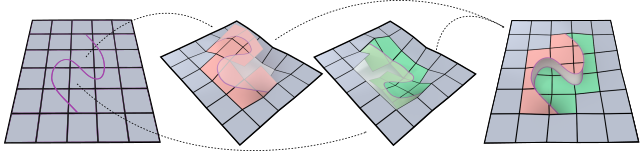
\includegraphics[width=.9\textwidth]{chapter_gridiron/images/New_HybridLattice2.pdf}
    % \includegraphics[width=.25\textwidth]{/tmp/foo.png}
    \vspace*{-.1in}
    \caption{Illustration of non-grid aligned topology change}{ A cutting path
    (far left) gives rise to new cells on either side of the cut
    (center), allowing the lattice to be divided below cell resolution
  (far right).}
    \vspace*{-.15in}
    \label{Fig:MaterialContinuityPreview}
  \end{figure}
  
  \section{Engineering A Solid Foundation}

  The following chapters will discuss in more detail some of the
  important engineering challenges and present techniques to overcome
  them. The primary goal is to demonstrate a set of related approaches
  that work well with each other and can be used to construct a highly
  performant, yet flexible foundation for a plastic surgery
  Simulation Assisted Visual System (SAVS). After a short related work section, highlighting some
  informative prior work, there will be several technical chapters
  dealing with the topics below. Finally, there will be a brief
  discussion section which will touch briefly on remaining
  philosophical issues and technical conclusions.

    \paragraph{Thin Feature Support}~ Due to the nature of the
      application, ensuring our simulated tissue can support thin
      geometric features, arising from incising tissue or simply the
      original tissue itself, is critical. What do we mean by support?
      In particular, our simulations need to be able to represent this
      geometry correctly within an embedded lattice deformer without
      compromising performance and accommodating behaviors like self
      collision. The current danger we face is that by embedding
      geometry in a lattice, instead of making our simulation elements
      conforming, we will not only loose accuracy around the boundary
      but potentially create unrealistic behavior by incorrectly connecting
      material across gaps unresolved by the lattice. In Chapters
      \ref{chp:nonmanifold} and \ref{chp:parallelization}, we'll look at
      solutions to these concerns via a process of non-manifold embedding.

    \paragraph{Optimized Lattice Deformers}~ We defined a
      SAVS to be an interactive system, and in order to use
      elastic simulation as a supporting technology we must ensure it
      can maintain sufficient levels of interactivity. Thus simulation
      performance is a key engineering challenge for us. Several times in this
      chapter we have mentioned that embedding lattice deformers were
      picked as the discretization model of choice over competing
      solutions, such as conforming mesh designs, due to their
      performance opportunities. These opportunities stem from their
      implicit data structures and regularity. These qualities reduce
      the amount of information than needs to read in order to access
      the store simulation data and allow for simplified computational
      designs.  However, these advantages do not come for free. In
      Chapters \ref{chp:parallelization} and \ref{chp:macroblocks}, we'll show
      how these properties can be exploited to create hardware aware
      algorithms for the solutions to the elasticity equations
      presented in this chapter. 
      
    \paragraph{Support for Non-linearity}~ While linear elastic
      materials are popular and easy to simulate, they fall short of
      the complexities observed in real biological material. While
      this document doesn't make any claim at delivering such
      materials, which require significant testing and validation
      against real tissue properties, we do wish to support these
      materials effectively. Moreover, even with relatively simple
      material models, adding additional constraints (either from
      user interactions or from contact) can make the problem
      non-linear. In Chapter \ref{chp:macroblocks}, we demonstrate a
      powerful generic technique for solving these highly non-linear
      problems, allowing for rapid convergence onto a correct
      solution.
      
    \paragraph{Deployment}~ While often overlooked, it is equally
      important to deliver a finished simulation to a user as it is to
      perform the simulation quickly and correctly. In Chapter
      \ref{chp:deployment}, we'll explore solutions for presenting
      simulated surgery operations to a multi-user environment. In
      particular, we'll look at issues such as available operating
      environments, suitability of cloud services, and maintainability.
   
  
  
%%% Local Variables:
%%% mode: latex
%%% TeX-master: "../document"
%%% End:




\chapter{Related Work}
\label{chp:relatedwork}

Faced with the challenge of providing an interactive virtual
environment for authoring plastic surgery simulations, the field of
computer graphics research has generated many potential solutions and
techniques to solve this problem. Procedural techniques
~\citep{JoshiMDGS:2007,WangP:2002,KavanCZO:2008,VaillBGCRWGP:2013} offer real-time
performance for certain animation tasks but lack the physical accuracy
needed in surgical simulations. Consequently, some research ventures
into surgical simulation turned to elastic deformation models
~\citep{TerzoPBF:1987} that responded more realistically to scenarios of
probing and cutting ~\citep{BroC:1996,MendoL:2003,NienhS:2001}. However,
these early works were limited in their scope and effectiveness due to
computational cost, geometric constraints and oversimplified material
models. In this section we outline prior contributions that help
address these limitations, and review a number of existing surgical
simulation systems.

\subsection{Simulation of Elastic Materials}

Simulation of elastic deformable models is ubiquitous in computer
graphics and remains a vibrant area of research. Algorithmic
techniques for deformable body simulation, pioneered by \citet{TerzoPBF:1987} have attained a significant level of
maturity, leading to broad adoption in visual effects, games, virtual
environments and biomechanics applications. Over the years, a number
of different approaches have been explored for the simulation of
deformable objects, each with different strengths. 

Lattice-based volumetric deformers are popular components in both
physics-based and procedural animation techniques. In the case of
physics-based simulation, one of their key advantages is that they
avoid having to construct a simulation-ready conforming volume mesh,
which is a delicate preprocessing task often requiring supervision and
fine-tuning. Another crucial benefit is that the regularity of such
data structures enables aggressive performance optimizations as
vividly demonstrated by shape matching techniques
~\citep{RiverJ:2007}. Cartesian lattices have also been leveraged to
accelerate performance in physics-based approaches, albeit
predominantly for simple models such as linear or corotated elasticity
~\citep{MuellTG:2004,GeorgW:2008,McAdaZSETTS:2011}. Prior graphics
work, however, has not demonstrated such aggressive performance gains
from lattice-based discretizations when highly nonlinear, anisotropic
or incompressible materials are involved. In part, this is attributed
to the fact that simulation of complex materials commands an increased
level of attention to issues of robust convergence. Mature solutions
to these concerns have predominantly been demonstrated in the context
of specific discretizations (e.g. explicit tetrahedral meshes) where
regularity of data structures, compactness of memory footprint and
parallelization/vectorization potential were not inherently
emphasized. Furthermore, as applications requiring the use of complex
materials are also likely to emphasize geometric accuracy, they often
opt for conforming mesh discretizations due to their superior
performance in capturing intricate boundary features, even if their
computational cost is higher.

Despite the popularity and feature set of conforming discretizations,
many researchers have explored improving embedded techniques for
reasons of simplicity and performance. Embedding has been combined
with homogenization ~\citep{NesmePF:2006,KhareMOD:2009} to resolve
sub-element variation of material parameters, optionally with the use
of non-manifold embedding lattices to support objects with a branching
structure ~\citep{NesmeKJF:2009}. 
\citet{JerabBBFA:2010} employed a method similar to the one
presented in Chapter \ref{chp:nonmanifold}, using a finer voxel grid
to capture material topology to be embedded in a coarser, non-manifold
voxel grid. Finally, \citet{ZhaoB:2013}
demonstrated the use of multiple voxel grid domains to segment a model
hierarchically, which they used to simulate plants at interactive
rates.

In addition to classical FEM approaches, some authors have
achieved success with more exotic variations. Extended FEM (XFEM)
formulations have also been explored ~\citep{JerabK:2009}, where
discontinuities are introduced into the element's shape functions, to
model cutting. In a similar vein,
\citet{KaufmMBG:2009} used discontinuous Galerkin FEM
formulations. Others have dispensed with mesh based discretizations
completely, preferring meshless methods ~\citep{DeB:2000} which were
also used for surgical simulation ~\citep{DeKLS:2005}.

\subsection{Anatomical Modeling}
Approaches based on the FEM have been particularly popular in the
medical simulation community ~\citep{MarchADC:2008} where the need for
biologically accurate materials is more pronounced. In one of the
earliest uses of advanced materials in computer animation, \citet{ChenZ:1992} focused on anatomical structures such
as muscles. FEM techniques were further leveraged in the animation
literature for the discretization of linear elasticity for fracture
modeling in a small-strain regime ~\citep{OBriH:1999}. Highly
nonlinear materials such as active musculature \citet{TeranBHF:2003}
exposed challenges in robustness and numerical stability of FEM
discretizations. Invertible FEM ~\citep{IrvinTF:2004} improved
simulation robustness in scenarios involving extreme compression,
while modified Newton methods ~\citep{TeranSIF:2005} reduced the cost
of implicit schemes with large time steps. Several of these algorithms
have been incorporated in open-source modeling and simulation packages
~\citep{SinSB:2013}. Solutions have also been proposed for material
behaviors such as incompressibility ~\citep{IrvinSF:2007} and
viscoelasticity ~\citep{GokteBO:2004,WojtaT:2008}, both of which can
be found in typical biomaterials.  Recent results in coupled
Lagrangian-Eulerian simulation of solids have also facilitated the
inclusion of intricate contact and collision handling in biomechanical
modeling tasks ~\citep{SuedaKP:2008,LiSNP:2013,FanLP:2014}.

\subsection{Topology Change}

A number of techniques have targetted topology change during
simulation, due to cutting or fracture. Early work ~\citep{TerzoF:1988b}
resorted to breaking connectivity of elements when stress limits were
exceeded. Later methods ~\citep{NienhS:2001} split tetrahedra near cut
boundaries and then used vertex snapping to more accurately
approximate the cut. Local remeshing was also employed to simulate
cracks in brittle materials ~\citep{OBriH:1999}. An issue with such
subdivision schemes is the possible creation of poorly conditioned
elements, which prompted a number of authors to pursue embedded
simulation schemes ~\citep{MolinBF:2004,TeranSBNLF:2005}. These
techniques use non-conforming meshes with elements which are only
partially covered by material, in lieu of conforming
remeshing. Embedded simulation can provide a great degree of
flexibility in cutting and fracture scenarios ~\citep{SifakDF:2007},
although cutting meshes along arbitrary surfaces requires delicate
book-keeping and careful handling of degeneracies.


\subsection{Surgical Simulation}
While much of the previously discussed work is geared towards general
elastic body simulation in computer graphics, many relevant results
originated in surgery-specific work. 
\citet{PiepeLR:1995} demonstrated a very early surgical simulation
platform for facial procedures, using FEM elastic shells.  Many
surgical simulation projects focus on the mechanical manipulation of
organs and other soft internal objects
~\citep{NienhS:2001,KimCDS:2007}. Even expensive commercial simulators
like the Lap Mentor and GI Mentor primarily focus on pushing and
cutting simulated internal organs
~\citep{SUSAC:2002--2014b,SUSAC:2002--2014}. These types of simulations
are so common that several open source frameworks have been built to
specifically support further development
~\citep{AllarCFBPDDGo:2007,CavusGT:2006}. These provide easy access to
common components like haptic feedback and APIs to connect multiple
simulated components. Certain surgical simulation systems are tailored
to specific skills, including interactive simulations of needle
insertion ~\citep{ChentARCHGSO:2009}.

\subsection{Performance Optimization}
Improving simulation rates is a common challenge for many interactive
modeling tasks, and even more so for accuracy-conscious applications
such as virtual surgery. Attempts to improve performance have either
relied on new data structures, faster solvers, or aggressive use of
parallelization. The Boundary Element Method ~\citep{JamesP:1999} has
been used to achieve interactive deformation rates for objects
manipulated via their surface. Other authors have employed similar
formulations that abstract away interior degrees of freedom to
accelerate collision processing ~\citep{GaoMS:2014}. Grid-based,
embedded elastic models
~\citep{MuellTG:2004,NesmePF:2006,McAdaZSETTS:2011,PatteMS:2012,MitchCS:2015}
have been very popular due to their inherent potential for performance
optimizations, and can also be used with shape-matching approaches
~\citep{RiverJ:2007}. They form the foundation for a class of highly
efficient, multigrid-based numerical solution techniques
~\citep{ZhuSTB:2010,GeorgW:2008,DickGW:2011}.  Regular discretizations
have also been coupled with multigrid solvers to facilitate GPU
accelerations for elastic skinning techniques ~\citep{McAdaST:2010}.
However, in spite of the efficiency of multigrid schemes, adapting
them to the presence of incisions or other intricate topological
features can be a nontrivial proposition.

\citet{HermaRF:2009} analyzed data flow in their
simulations to inform a parallel scheduler for multicore systems. To
avoid write hazards during parallel code execution, 
\citet{KimP:2011} proposed a system of computation phases with
coalesced memory writes, which allowed them to parallelize force
computation. Related efforts by 
\citet{CourtA:2009}, developed a parallel version of the
Gauss-Seidel algorithm that can run on GPUs. Finally, optimized direct
solvers have been shown to be very effective ~\citep{SinSB:2013} and
have employed techniques such as delayed updates to factorization
approaches ~\citep{HechtLSO:2012} for improved efficiency. The
approach outlined in Chapter \ref{chp:macroblocks} is related to these
approaches, as well as the general class of Schur complement methods
~\citep{QuartV:1999}.

\subsection{Level Sets and Collision Handling}

Level set methods were first introduced by \citet{OsherS:1988} for tracking moving interfaces in the
context of Hamilton-Jacobi equations.  Subsequently, \citet{AdalsS:1994} proposed substantial runtime savings
by restricting computations to a thin band of active voxels near the
interface.  \citet{Sethi:1998} proposed fast marching
methods for monotonically advancing fronts as well as for redistancing
the level set using values seeded only on the narrow band.  Besides
fast computation, a number of methods have also been proposed for
efficiently storing level sets including octrees~\citep{LosasGF:2004},
RLE representations~\citep{HoustNBNM:2006,IrvinGLF:2006,ChentM:2011},
the VDB data structure~\citep{Muset:2013} which evolved from Dynamic
Tubular Grids~\citep{NielsM:2006} and the DB+Grid data
structure~\citep{Muset:2011}, and the virtual-memory based SPGrid data
structure~\citep{SetalABS:2014}.

Methods have been proposed for computing implicit representations of
non-manifold surfaces~\citep{BloomF:1995,YuanYW:2012}. Similar ideas
were used for simulating bubbles~\citep{ZhengYP:2006} and multiphase
fluids~\citep{LosasSSF:2006}. The work in Chapter \ref{chp:nonmanifold}
diverges from these approaches as we enhance the expressive capability
of a \emph{single} level set by embedding signed distance values on an
explicit mesh. Our work is related to the practice of embedding
high-resolution geometry in regular meshes, a concept that was first
leveraged by \citet{MulleTG:2004} for deformable
body simulations and fracture.  In addition to hexahedral embeddings,
methods such as the virtual node algorithm~\citep{MolinBF:2004} have
been used to create non-manifold tetrahedral lattices that correspond
to thin topological features in the embedding geometry. Virtual node
concepts are also similar to XFEM methods which were used for crack
modeling~\citep{MoeesDB:1999} and for cutting and fracturing thin
shells~\citep{KaufmMBGG:2009}. This principle has continued to evolve
with many of the topological limitations in prior approaches being
raised by \citet{SifakDF:2007} and has been
successfully used in production tools as well~\citep{HellrSSST:2009}.

Our non-manifold level set approach in Chapter \ref{chp:nonmanifold}
is inspired by these methods, but it needs to be made cognizant of
further topological limitations that the signed distance field imposes
on our representation (see
Section~\ref{sec:non-manifold-level-sets}). Notably, when dealing with
collisions near thin features, all of the aforementioned approaches
employed detection and response techniques based on surface
meshes~\citep{BridsFA:2002} that rely on the availability of good
surface meshes, are computationally expensive, presume collision-free
history or use impulses which makes implicit integration
challenging. To accelerate collision detection and response while
allowing for implicit integration, methods have been proposed using
implicit surface representations~\citep{McAdaZSETTS:2011} which work
even in near-interactive settings, but require enough level set
resolution to avoid any non-manifold features altogether. Recently,
image-based techniques~\citep{FaureBAF:2008,WangFP:2012} have been
proposed which provide an interesting alternative.  Finally, implicit
surfaces have also been recently used in real-time skinning
applications~\citep{VaillBGCRWGP:2013,VaillGBWC:2014}.


%%% Local Variables:
%%% mode: latex
%%% TeX-master: "../document"
%%% End:


%%%%%%%%%%%%%%%%%%%%%%%%%%%%%%%%%%%%%%%%%%%%%%%%%%%%%%%%%%%%%%%%%%%%%%%%
%%%%%%%%%%%%%%%%%%%%%%%%%%%%%%%%%%%%%%%%%%%%%%%%%%%%%%%%%%%%%%%%%%%%%%%%
%%%%%%%%%%%%%%%%%%%%%%%%%%%%%%%%%%%%%%%%%%%%%%%%%%%%%%%%%%%%%%%%%%%%%%%%
%                         PAPER CHAPTERS
%%%%%%%%%%%%%%%%%%%%%%%%%%%%%%%%%%%%%%%%%%%%%%%%%%%%%%%%%%%%%%%%%%%%%%%%
%%%%%%%%%%%%%%%%%%%%%%%%%%%%%%%%%%%%%%%%%%%%%%%%%%%%%%%%%%%%%%%%%%%%%%%%
%%%%%%%%%%%%%%%%%%%%%%%%%%%%%%%%%%%%%%%%%%%%%%%%%%%%%%%%%%%%%%%%%%%%%%%%

\chapter{Non-manifold Embedding for Geometry and Contact}
\label{chp:nonmanifold}

\section{Non-manifold Embedding}
\label{sec:hybrid}

\begin{figure}
  \centering
  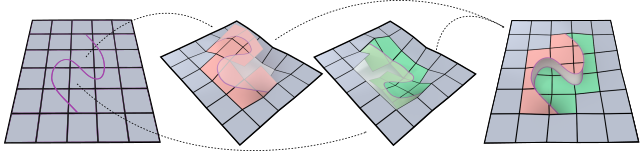
\includegraphics[width=.9\textwidth]{chapter_gridiron/images/New_HybridLattice2.pdf}
 % \includegraphics[width=.25\textwidth]{/tmp/foo.png}
\vspace*{-.1in}
\caption{Illustration of a cut generating a non-manifold lattice}{ (a) A cut
  passing through the grid. (b) Mesh cells generated for the top half
  of the cut. (c) Mesh cells generated for the bottom half of the
  cut. (d) Cut surface is colored to show cell assignment.}
\vspace*{-.15in}
\label{Fig:MaterialContinuity}
\end{figure}

We employ an embedded simulation similar to other authors, who used
regular lattice embeddings for performance
\cite{MuellTG:2004,RiverJ:2007,McAdaZSETTS:2011}. However, due to the
presence of extremely thin incisions common in surgical models, standard
lattice embedding would not be able to resolve the tissue topology,
unless an extremely high resolution embedding was used. We thus adopt
a non-manifold lattice-derived embedding discretization in the spirit
of Virtual Node or XFEM methods
\cite{MolinBF:2004,SifakDF:2007,NesmeKJF:2009}.  In this chapter, we
describe how these non-manifold embedding structures can be easily
constructed and how they can be used for handling contact scenarios in
addition to geometry representation. The following chapter will
discuss how these structures can be further optimzed for parallel
processing.

\subsection{Surface Model}

\begin{figure}
\vspace*{-.23in}
  \centering
  \includegraphics[width=.45\columnwidth]{chapter_gridiron/images/Uncut_Surface_Model2.png}
  \includegraphics[width=.45\columnwidth]{chapter_gridiron/images/Cut_Surface_Model2.png}
\vspace*{-.12in}
  \caption{Illustration of incision technique}{Incisions in the flesh surface model are created by extruding and thickening user specified line segments.}
\label{fig:incision}
\end{figure}

Prior to elasticity discretization, a watertight surface model of the
flesh, including any incisions, must be created. The method choosen to
generate these models is immaterial to our embedding algorithm, but
for completeness we present our solution for incising surgical tissue
models. In our system, incisions are generated from user specified
line segment curves, which guide constructive solid geometry (CSG)
difference operations to produce cut surface meshes.  We begin from a
user specified line segment curve from which we construct prisms by
thickening the line segments tangentially and perpendicularly along
the surface normal. We then apply these prisms in a subtraction
operation with the surface, resulting in a slightly thickened incision
(Figure \ref{fig:incision}). Disconnected regions produced during this
step can be marked and removed by the user. Note that for scenarios
involving malignant tissue, discarding of excised tissue is
commonplace.

\subsection{Rasterization}

\begin{figure}
  \centering
  \vspace*{-.25in}
  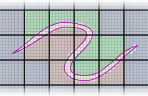
\includegraphics[width=\columnwidth]{chapter_gridiron/images/Figure_Topology_C}
\vspace*{-.3in}
  \caption{Illustration of the fine grid rasterization of a cut}{Fine cells within the cut are empty, and colored to show material continuity.}
\label{Fig:CuttingFineGrid}
\end{figure}

Given a cut surface mesh, we first create a fine rasterization of the
surface. The resolution of the rasterization is selected to capture
all desired topological detail (typically an order of magnitude finer
than simulation resolution). In Figure \ref{Fig:CuttingFineGrid}, it
is possible to see the fine rasterization grid in contrast to the
coarser simulation resolution.  The rasterization is performed by
detecting all voxels intersected by the object surface and
flood-filling to mark the volumetric material region.  Once the
rasterization is complete, subsequent embedding operations are purely
combinatorial, and not sensitive to poor conditioning of surface mesh
elements.  Additionally, this fine-grid embedding can also act as an
interface layer to more complex embedding schemes, such as the
non-manifold approach described next. We leverage this by translating
any deformation results back to the fine-grid embedding prior to
rendering, to hide non-manifold embedding or numerical solution
details from the visual front-end.

\subsection{Non-Manifold mesh generation}
\label{sec:nonmanifoldmeshgeneration}

We now seek to construct a coarser resolution explicit mesh
discretization, which is allowed to be non-manifold in regions, as
shown in Figure \ref{Fig:MaterialContinuity}. We will extend the
paradigm of non-manifold embedding proposed by Teran et al.\!
\shortcite{TeranSBNLF:2005} and Sifakis et al.\!
\shortcite{SifakDF:2007} using the precomputed fine grid rasterization
to answer material connectivity predicates. Our non-manifold mesh
generation process is outlined in Algorithm
\ref{alg:NonmanifoldMeshGeneration}, and illustrated intuitively in
Figure \ref{Fig:MaterialContinuity}. Note that, in the pseudocode
provided, there are two geometric predicates being used: (a)
Determination of material components (line 3) requires the
identification of all disconnected components of material present in
the intersection of our domain with a given lattice cell. (b)
Adjacent-element material continuity (line 10) is a predicate invoked
to determine if two material fragments, associated with adjacent
lattice cells, exhibit material continuity across their common
face. These two geometric predicates are expressed in a fashion that
is agnostic to the underlying geometric representation of material; in
Teran et al.\! \shortcite{TeranSBNLF:2005} the assumption is that a
tetrahedralized model of the material is available, while Sifakis et
al.\! \shortcite{SifakDF:2007} define material fragments indirectly,
by specifying cutting surfaces instead. In our case, the availability
of the fine-grid rasterization makes both such operations purely
combinatorial in nature. Material fragments within a coarse cell are
computed via flood-fill, and fragments on adjacent cells are
continuous if they contain adjacent \emph{fine} cells on their
rasterization. At the conclusion of this step, we have produced a
coarse mesh (with explicitly stored connectivity), whose topology is
as close as possible to the embedded geometry.

This generated mesh is now suitable for simulation, allowing us to
correctly embed opposite sides of a cut or thin feature in
topologically disconnected cells. However, beyond simulation, this
approach can also be valuable for detecting and handling contact
scenarios under the context of soft-body self collisions. The
remaining sections in this chapter will demonstrate how this embedding
technique can be adapted to this purpose via a technique we call
non-manifold level sets.

\begin{algorithm}
  \caption{Non-Manifold Simulation Mesh Construction}{This algorithm
    describes the steps required to identify material connectivity
    across voxel boundaries, and generate appropriate voxel topologies
    which respect this underlying material toplogy. Material
    continuity across voxel faces results in vertex collapse. While
    this can lead to loss of simulation resolution near incision
    points, it doesn't affect the embedding process and is less
    complicated to simulate. }
\label{alg:NonmanifoldMeshGeneration}
\begin{algorithmic}[1]
\Require Coarse Resolution
\Function{Generate$\_$Nonmanifold$\_$Mesh}{}

  \ForAll{Coarse Cells: $i$}
     \State $C$ $\gets$ \Call{Determine$\_$Material$\_$Components}{$i$}
     \ForAll{ Components in $C$ }
     \State Instance separate copy of $i$
     \State Generate unique, separate DOFs
     \State Assign descriptor of material content
  \EndFor
\EndFor

   \ForAll{Geometrically adjacent cell pairs: $(i, j)$}
      \ForAll{Pairs of duplicates from $i$ and $j$: $(h, k)$}
         \If{ \Call{Material$\_$Is$\_$Continuous}{$h$, $k$} }
            \State Mark shared vertices as equivalent
         \EndIf
      \EndFor
   \EndFor

   \ForAll{Coarse Cells: $i$}
      \State Compare all duplicates of $i$
      \State Collapse duplicates with equivalent DOF's
   \EndFor
\EndFunction
\Ensure An explicit, possibly non-manifold mesh
\end{algorithmic}
\end{algorithm}

\section{Level Sets \& Collision Processing}
Before we discuss the details of non-manifold levelsets, it is
important to review the basic concept of a level set and how it can be
used for collision handling. Nearly three decades after their
introduction \cite{OsherS:1988}, level sets have evolved into one of
the most widely used representations of geometry, alongside
traditional alternatives such as meshes, splines and subdivision
surfaces. A level set implicitly represents a domain boundary
$\Gamma=\partial\Omega$ as the zero-value isosurface (i.e. zero
\emph{level set})
\begin{equation}
\Gamma=\left\{\vec{x}\in\mathbf{R}^n\ |\ \phi(\vec{x})=0\right\}
\label{eqn:definition}
\end{equation}
of a scalar field $\phi(\vec{x})$ measuring signed distances to the
boundary of the object $\Omega\subset\mathbf{R}^n$. Level sets allow
for fast $O(1)$ time point-object intersection queries or point
projections to the object surface. Model deformation is also possible,
including topological split and merge operations, simply by varying
the underlying scalar field. Level sets are used in a diverse range of
applications including surface editing \cite{MusetBWB:2002},
tetrahedral meshing \cite{LabelS:2007}, scattered point interpolation
\cite{ZhaoOF:2001}, fluid simulation \cite{OsherF:2002} and collision
processing for deformable solids \cite{Gascu:1993}, rigid bodies
\cite{GuendBF:2003} and skinning animations \cite{VaillBGCRWGP:2013}.


\begin{figure}
  \centering
\includegraphics[width=0.98\columnwidth]{chapter_nonmanifoldlevelsets/images/problem_cases.pdf}
\vspace*{-.15in}
\caption{Illustration of cases poorly handled by conventional level
  set discretizations} {Scenarios where standard Cartesian grid-based
  level sets lack the expressive ability to resolve thin features. For
  the vector art hand (top left), the cells highlighted in red show
  features that will not be resolved. While many cases can be resolved
  with fine enough resolutions, the fractured cube (bottom left) is an
  instance that cannot be resolved with conventional level sets.}
\label{fig:underresolved}
\vspace*{-.2in}
\end{figure}


% The algorithmic interface to an implicit surface data structure is
% highly dependent on the application it caters to. A fluid simulation
% application would likely mandate support for dynamic evolution of the
% interface. Geometry processing tasks may be more dependent on
% contouring or differential properties such as curvature. The data
% structure we propose, which is essentially a multivalued signed
% distance field, might require a different interface depending on the
% end application. For example, applications in multiphase
% fluids~\cite{LosasSSF:2006}, multi-material surface
% tracking~\cite{DaBG:2014} or volumetric meshing~\cite{SachtJPSS:2013}
% may contribute their own interpretations to what a non-manifold
% feature may be and what algorithmic routines need to be supported.

% The algorithmic interface of different instances of level set methods
% is highly dependent on the applications they cater to. When seeking
% unconventional extensions to the core level set formulation, it is
% important to recognize that the semantics of a \emph{multivalued or
%   non-manifold level set} can invite quite distinct interpretations in
% different use scenarios. For example, fluid simulation of multiple
% immiscible liquids \cite{LosasSSF:2006} might consider triple
% junctions as a ``non-manifold'' trait of interest, while fluid
% animations that allow different liquids to diffuse into one another
% might require modeling phase boundaries that can cross and overtake
% one another. Similarly, applications in shape modeling and collision
% processing might not concern themselves with advection tasks, but
% emphasize the signed distance property and the geometric queries it
% facilitates.

% In order to avoid such ambiguities we focus our scope to a specific
% driving application: collision detection and penalty-based response on
% volumetric simulation of elastic solids.  In section
% \ref{sec:self-collisions} we review how this specific application
% utilizes conventional (manifold) level sets, identify scenarios where
% the limitations of the traditional formulation hinder the efficacy of
% collision processing or even make it inapplicable, and explain how the
% non-manifold level set concept can alleviate those obstacles.  In
% summary, our key contributions are as follows:

% While the visual fidelity of fluid simulations is not severely
% compromised even though level sets bleed resolution, solid
% simulations run into problems when two surfaces come very close to
% each other.  This issue can arise either due to collisions or be
% inherent in the model itself (for e.g., lips, fingers and armpits in
% a human model). Interestingly, we observe that these issues are not
% intrinsic to the concept of the level set function, but rather the
% data structure that is typically used for storage.  By convention
% (or habit), standard arrays are used for storage as opposed to
% something more expressive. Normally, a level set function captures
% the (signed) distance to the surface.  By changing the underlying
% data structure, we aim to extend the definition of a level set so
% that it can capture distance to several local minima of closest
% points as well as distance to the surface along a given connectivity
% path. (Maybe refer to a figure for the lips here?)

% Self-collision in volumetric bodies gives rise to interesting
% options: a) only the surface need be processed (while elasticity
% takes care of the rest), and b) as opposed to cloth
% simulations~\cite{BarafWK:2003}, the starting state need not be
% interpenetration-free - these facts have been leveraged in
% conjunction with level sets~\cite{TeranSIF:2005,McAdaZSETTS:2011}
% even in performance-conscious environments and have proven to be
% robust in resolving extremely complex collision scenarios such as
% triple contacts. However, a significant limitation of this approach
% is that it requires the reference configuration of an object to be
% level set representable. While this is possible in some cases, it
% becomes challenging in other situations such as the lips which
% require an incredible amount of resolution to resolve the gap in
% between (note that this resolution is not required for either the
% upper lip or the lower lip in isolation, or if both lips were
% initially far apart). This problem also arises when simulating
% incisions or fracture. Similar challenges arise in applications such
% as meshing techniques that use level set representations as the
% input, in such cases an exorbitant amount of resolution might be
% required near topological features that need to be resolved in a
% voxelization of the domain.  Embedded representations suffer from
% similar problems as they have to stick to the topology of the
% embedding lattice. Our motivation comes from virtual node/XFEM
% descriptions that alleviate these issues by using a non-manifold
% mesh to capture the domain augmented with some kind of a sub-cell
% description of the domain (or its boundary). Our key idea is to use
% a fracture modeling algorithm to create a non-Euclidean embedded
% mesh structure for storing the level set function. We also show how
% peripheral operations such as reinitialization, advection and
% contouring can be extended to this new data structure.


% \begin{itemize}
% \vspace*{-.04in}\item We extend level set representations by storing
% discrete values on nodes of a non-manifold Cartesian grid, enabling
% them to represent domains with thin gaps or slivers, and even encode
% boundaries of overlapping material domains.

% \vspace*{-.08in}\item We detail a systematic pipeline for converting
% mesh-based geometry representations into multivalued level sets, and
% discuss how other geometric descriptions
% % (e.g. fracture boundaries)
% could also be used as input.

% \vspace*{-.08in}\item We extend a number of algorithmic concepts and
% geometric predicates, such as signed distance initialization and
% closest-point projection to the non-manifold level set paradigm.

% \vspace*{-.08in}\item We show how non-manifold level sets can
% broaden the scope of penalty-based self-collision processing for
% elastic solids.

% \end{itemize}
% \vspace*{-.1in}

% \section{Previous work}
% \vspace*{-.1in}
% \label{sec:previous-work}

% Level set methods were first introduced \changed{by Osher and
%   Sethian~\shortcite{OsherS:1988}}{in~\cite{OsherS:1988}} for tracking
% moving interfaces in the context of Hamilton-Jacobi equations.
% Subsequently, \changed{Adalsteinsson and
%   Sethian~\shortcite{AdalsS:1994}}{\cite{AdalsS:1994}} proposed
% substantial \changed{runtime savings }{savings to the run-time }by
% restricting computations to a thin band of active voxels near the
% interface.
% \changed{Sethian~\shortcite{Sethi:1998}}{\cite{Sethi:1998}} proposed
% fast marching methods for monotonically advancing fronts as well as
% for redistancing the level set using values seeded only on the narrow
% band.  Besides fast computation, a number of methods have also been
% proposed for efficiently storing level sets including
% octrees~\cite{LosasGF:2004}, RLE
% representations~\cite{HoustNBNM:2006,IrvinGLF:2006,ChentM:2011}, the
% VDB data structure~\cite{Muset:2013} which evolved from Dynamic
% Tubular Grids~\cite{NielsM:2006} and the DB+Grid data
% structure~\cite{Muset:2011}, and the virtual-memory based SPGrid data
% structure~\cite{SetalABS:2014}.

% Methods have been proposed for computing implicit representations of
% non-manifold surfaces~\cite{BloomF:1995,YuanYW:2012}. Similar ideas
% were used for simulating bubbles~\cite{ZhengYP:2006} and multiphase
% fluids~\cite{LosasSSF:2006}. Our work diverges from these approaches
% as we enhance the expressive capability of a \emph{single} level set
% by embedding signed distance values on an explicit mesh. Our work is
% related to the practice of embedding high-resolution geometry in
% regular meshes, a concept that was first leveraged \changed{by
%   M\"{u}ller et al.~\shortcite{MulleTG:2004}}{in~\cite{MulleTG:2004}}
% for deformable body simulations and fracture.  In addition to
% hexahedral embeddings, methods such as the virtual node
% algorithm~\cite{MolinBF:2004} have been used to create non-manifold
% tetrahedral lattices that correspond to thin topological features in
% the embedding geometry. Virtual node concepts are also similar to XFEM
% methods which were used for crack modeling~\cite{MoeesDB:1999} and for
% cutting and fracturing thin shells~\cite{KaufmMBGG:2009}. This
% principle has continued to evolve with many of the topological
% limitations in prior approaches being raised \changed{by Sifakis et
%   al.~\shortcite{SifakDF:2007}}{in~\cite{SifakDF:2007}} and has been
% successfully used in production tools as well~\cite{HellrSSST:2009}.

% Our non-manifold level set approach is inspired by these methods, but
% it needs to be made cognizant of further topological limitations that
% the signed distance field imposes on our representation (see
% Section~\ref{sec:non-manifold-level-sets}). Notably, when dealing with
% collisions near thin features, all of the aforementioned approaches
% employed detection and response techniques based on surface
% meshes~\cite{BridsFA:2002} that rely on the availability of good
% surface meshes, are computationally expensive, presume collision-free
% history or use impulses which makes implicit integration
% challenging. To accelerate collision detection and response while
% allowing for implicit integration, methods have been proposed using
% implicit surface representations~\cite{McAdaZSETTS:2011} which work
% even in near-interactive settings, but require enough level set
% resolution to avoid any non-manifold features altogether. Recently,
% image-based techniques~\cite{FaureBAF:2008,WangFP:2012} have been
% proposed which provide an interesting alternative.  Finally, implicit
% surfaces have also been recently used in real-time skinning
% applications~\cite{VaillBGCRWGP:2013,VaillGBWC:2014}.

\subsection{Level set collisions for volumetric solids}
\label{sec:self-collisions}

% We present our new implicit surface formulation in the context of
% collision processing for elastic volumetric bodies.

Self-collision processing is paramount in generating visually attractive and
realistic shapes, as is evident in character skinning pipelines
\cite{McAdaZSETTS:2011,VaillBGCRWGP:2013}. Handling collisions in
volumetric solids can be quite different than the typical cloth
collision pipeline. With volumetric solids there is a clear
distinction between an \emph{inside} and an \emph{outside} region,
making it possible to process collisions in a single time instance of
a simulated deformation. In contrast, if collisions are detected in a
cloth simulation, we need to rely on deformation history to determine
how the cloth surface is to be untangled (unless global intersection
analysis~\cite{BarafWK:2003} is performed). While cloth simulations
typically strive for a collision-free state at all times, commonly
enforced via impulses in semi-implicit integration
schemes~\cite{BridsMF:2003}, volumetric objects can tolerate
occasional, limited interpenetration, and respond to collision with
penalty forces which are more easily coupled with explicit integration
schemes. In this section, we review a level-set assisted technique
that capitalizes on these opportunities to handle volumetric object
collisions in large time-step implicit integration schemes, without
requiring a collision-free deformation history.  In section
\ref{sec:non-manifold-level-sets} we explain when standard level sets
are inadequate for this task, and use this as motivation for our
non-manifold variant.

\begin{figure}
  \centering
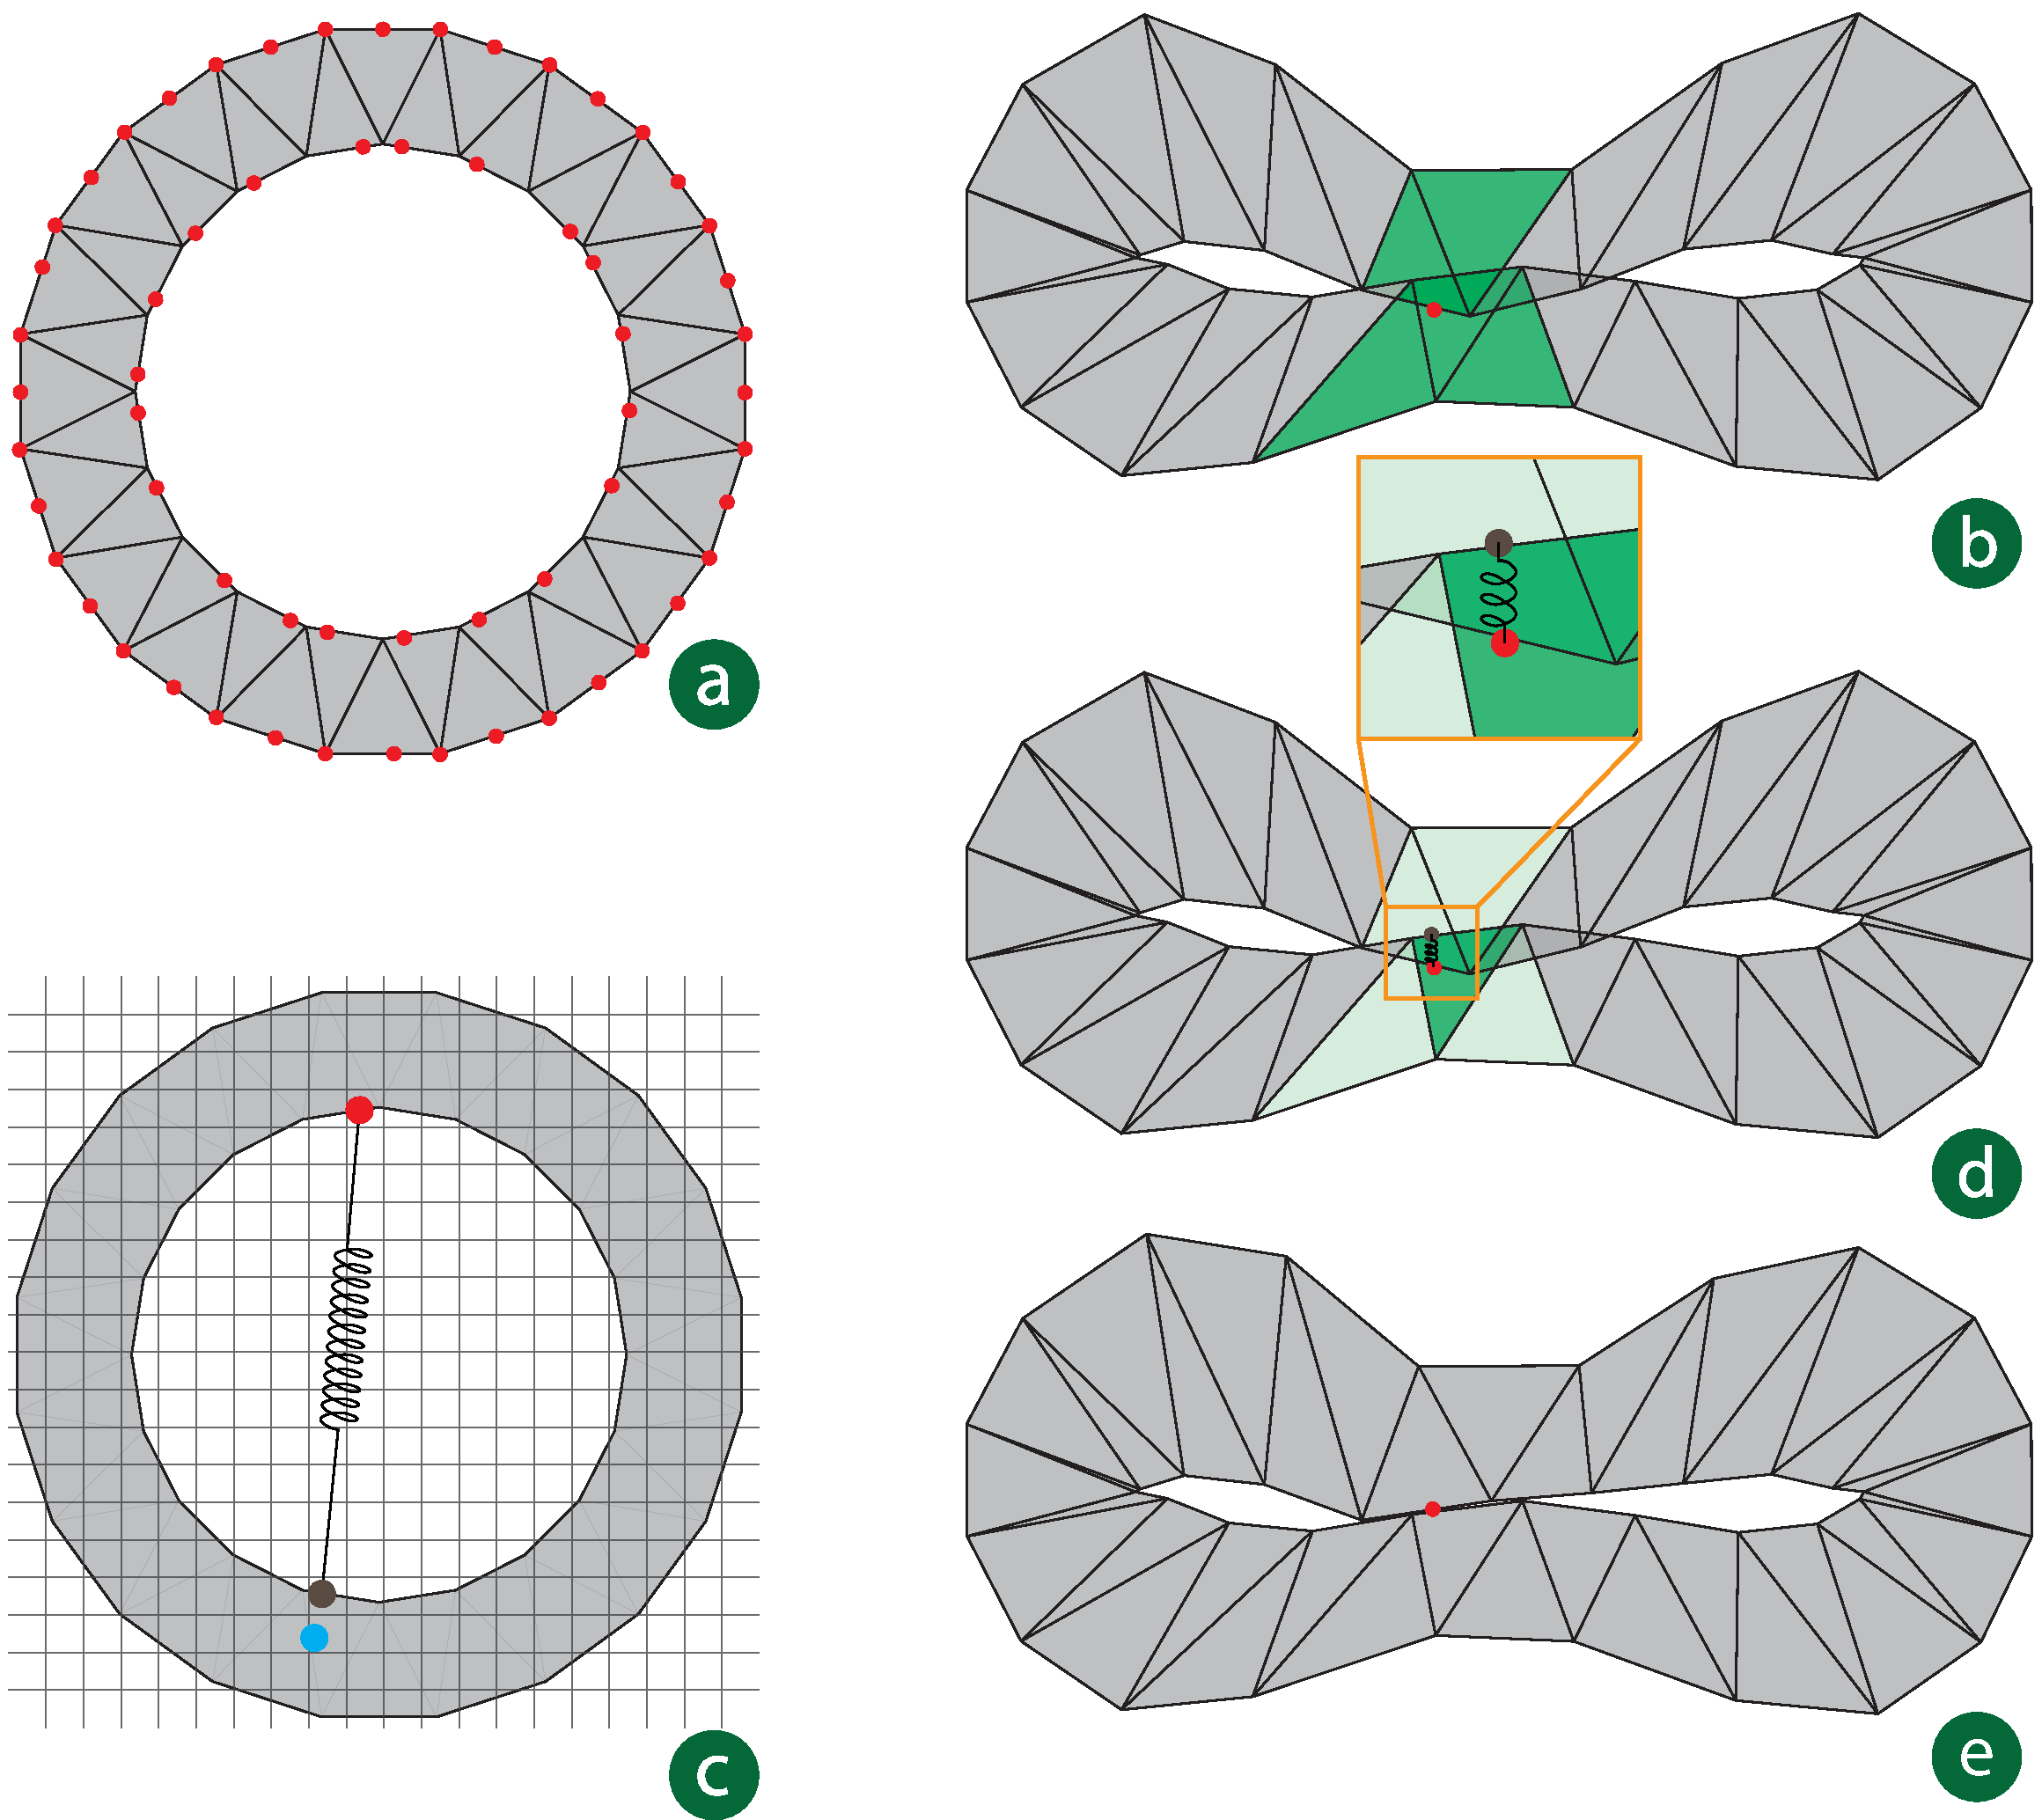
\includegraphics[width=0.95\columnwidth]{chapter_nonmanifoldlevelsets/images/torus-combined-latest.pdf}
\vspace*{-.1in}
\caption{Illustration of the self-collision pipeline}{(a) a
  triangulated torus model is pictured in its undeformed
  configuration. Collision proxies on the surface shown in red.  (b)
  The torus is deformed into a self-colliding state. A bounding box
  hierarchy yields initial candidates of triangles colliding with the
  proxy.  (c) After pruning false positives, the material location
  that the proxy collided onto is identified, and mapped back to the
  undeformed configuration (blue dot). The level set (stored on the
  pictured grid) is used to project to the closest surface point
  (brown dot).  (d) A zero-rest spring is initialized between the
  proxy and its surface-projected target.  (e) The deformed torus
  after the self-collision is resolved.}
\label{fig:self-collision-handling}
\vspace*{-.2in}
\end{figure}


Our collision pipeline consists of two stages: In the detection stage,
discrete material points (labeled \emph{collision proxies}) are
checked for collision against the object interior. In the response
stage, we use a spring-like penalty force to push each colliding proxy
to the object surface~\cite{TeranSIF:2005,McAdaZSETTS:2011}. Since
simulated solids are typically endowed with elastic material models
that prevent (or discourage) inversion, in all our examples we chose
to only seed collision proxies on the object surface, as internal
non-inversion combined with boundary non-collision would imply a
globally non-intersecting state. Interior collision proxies can also
be used, if desired, with no algorithmic
change. Figure~\ref{fig:self-collision-handling} illustrates the
detection and response process on an elastic torus model squished into
self-collision. For any colliding proxy, we identify the offending
(internal) material location that the proxy collided with. The closest
surface point to that material location is calculated, and a zero
rest-length spring is introduced between that surface location and the
original proxy. This spring remains active just until the collision
detection phase is repeated; typically for one step of the time
integration method employed, or for just a single Newton iteration in
an implicit scheme. The most costly predicates in this process are (i)
detecting whether a proxy intersects the object interior, and (ii)
projecting the offending location to the model surface. Both
predicates could be answered in $O(1)$ if a level set representation
of the model was available; unfortunately, the continuous deformation
makes updating an implicit representation impractical. Hence, we opt
for an \emph{approximate} algorithm ~\cite{McAdaZSETTS:2011} that only
relies on a level set representation of the \emph{undeformed} model.

For simplicity, let us assume that the deformable volumetric solids
are tetrahedralized (we can make this choice without loss of
generality - the following algorithm applies equally well to
hexahedral discretizations). Let $E_i$ denote the $i$-th simulation
element in the undeformed configuration and $e_i$ denote the same
element in the deformed configuration. Similarly, let $P_i$ denote the
location of the $i$-th collision proxy in the undeformed configuration
and $p_i$ denote its deformed counterpart.  Collision proxies can be
regularly sampled on the \emph{surface} of the simulated object, or
the surface vetices of the embedded object themselves can be used as
proxies, if their distribution is reasonably regular\footnote{Proxy
  spacing is an important task, though not particularly important for
  this conversation. Too few proxies in a region can lead to poor
  collision response or excessive penteration. Too many proxies can
  lead to an overconstrained problem, resulting in slow convergence or
  other unfortunate artifacts. For our system, a possion-disk
  sampling technique \cite{CorsiCS:2012}\cite{Devro:1986} was used to generate a blue noise pattern
of proxies over the model surfaces.}.  Let $\phi$
denote the level set function for the simulated volume in the
undeformed configuration. The collision handling routine performs the
following steps for each proxy $p_i$\ :

\textbf{Step 1}\ \ The set of (deformed) elements $\mathcal
  E=\{e_{i_1},e_{i_2},\ldots,e_{i_k}\}$ are checked against $p_i$ for intersection. This is performed as follows:

  \begin{enumerate}[(a)]
    \vspace*{-.07in}\item We use an axis-aligned bounding box
    hierarchy, defined over all deformed elements, to identify all
    elements whose bounding box intersects $p_i$, i.e.\
    $\mathcal{E}_{\mbox{\small
        int}}=\{e_k\in\mathcal{E}|\texttt{Box(}e_k\texttt{)}\cap
    p_i\neq\emptyset\}$.

    \vspace*{-.07in}\item We identify the element $E_i$ that contains the proxy
    $P_i$ in the undeformed configuration. This may be more than one element,
    e.g.\ if $P_i$ was a mesh vertex. We trivially have that
    $e_i\in\mathcal{E}_{\mbox{\small int}}$, as $p_i$ is embedded in it.
    Similar to McAdams et al.~\shortcite{McAdaZSETTS:2011}, we prune $e_i$ along with all of its immediate topological neighbors from
    $\mathcal{E}_{\mbox{\small int}}$, since collision response between
    primitives that share embedding parents can be problematic (we rely on
    elasticity instead, to discourage extreme cases of local collision).

% Element $e_i$ and its topological neighbors
%    are discarded from the computed set, where $P_i$ is embedded
%    inside $E_i$ in the rest configuration. This is done to prune
%    false negatives, as the proxy will trivially intersect its own
%    topological neighborhood.

    \vspace*{-.07in}\item We perform an exact intersection test
    between any elements $e_t$ that have not been already pruned. We
    do so by computing the barycentric coordinates of $p_i$ with
    respect to $e_t$, and discard elements if those coordinates are
    out of bounds.

  \end{enumerate}
  \vspace*{-.07in} \textbf{Step 2}\ \ For every colliding proxy, we
  identify the location $X_t$ in the \emph{undeformed} configuration
  of the material point the proxy impacted\footnote{Note that the location $X_t$ is unique if the element
$E_t$ is a triangle in two spatial dimensions or a tetrahedron in
three spatial dimensions, but this may not be the case for polygonal
or polyhedral elements such as squares, hexahedra, etc. We first
triangulate or tetrahedralize such elements, which can result in
several locations $\{X_{t_1},X_{t_2},\ldots,X_{t_r}\}$ in the rest
configuration corresponding to each of these several
triangles/tetrahedrons. In this case, we initialize the spring between
$p_i$ and the point $y_{t_j}$, where $X_{t_j}$ is \emph{closest} to
the surface.}. We do so using the
  barycentric coordinates computed in step 1(c) to interpolate $X_t$
  from the \emph{undeformed} colliding element $E_t$.
  \\
  \textbf{Step 3}\ \ Elements $E_t$ with $\phi(X_t)\!\!>\!\!0$ are
  dismissed as non-colliding (this could be due to discretization
  discrepancy between mesh and level set, or if an embedded simulation
  approach is used where elements in $\mathcal{E}$ reach beyond the
  extent of the simulated model).
  \\
  \textbf{Step 4}\ \ Using the level set, point $X_t$ is projected to
  the surface point $Y_t=X_t\!-\!\phi(X_t)\nabla\phi(X_t)$, for all
  elements $E_t$, where $e_t\in\mathcal{E}_{\mbox{\small int}}$.
  \\
  \textbf{Step 5}\ \ In the deformed configuration, a zero rest-length
  spring is initialized between points $p_i$ and $y_t$ to resolve the
  collision.

%\vspace*{-.2in}
  In step 5, $y_t$ corresponds to the point $Y_t$ in the deformed
  configuration.  Note that our algorithm, in steps 3 and 4, relied
  upon a level set representation of the \emph{undeformed} shape of
  the simulated model. The cost paid for this convenience is that the
  surface location $y_t$ (the collision target) is only an approximate
  surface projection in the \emph{deformed} configuration;
  nevertheless, this disparity vanishes as the effect of the collision
  springs progressively brings the penetration depth closer to zero.

Figure~\ref{fig:self-collision-handling} illustrates the
individual steps of the algorithm on a torus in two spatial
dimensions.


\section{Non-manifold Level Sets}
\label{sec:non-manifold-level-sets}

In principle, based on equation (\ref{eqn:definition}) a level set
could represent any object $\Omega\subset\mathbf{R}^n$. In practice,
however, the scalar field $\phi(\vec{x})$ is never provided
analytically, but sampled instead at discrete points in
$\mathbf{R}^n$. As a consequence, the expressive ability of discrete
level sets is limited by the sampling resolution and the interpolation
scheme used. In the common practice where $\phi$ values are sampled on
the nodes of a uniform Cartesian grid, and trilinear interpolation is
used to define a continuous scalar field, models with multiple
boundary crossings per grid edge (near narrow gaps or strips, see
Figure~\ref{fig:underresolved}) cannot be represented. These issues
can be alleviated to some extent by using adaptive schemes
\cite{LosasGF:2004,Muset:2013} to concentrate resolution near fine
features, or hybridizing with point-based methods \cite{EnrigMF:2002}
to capture details at a sub-cell level. Nevertheless, gratuitously
increasing the level set sampling resolution is a brute-force remedy
which quickly becomes impractical if the thickness of topological gaps
approaches zero, as is commonly the case with geometries arising from
cutting and fracture modeling pipelines (see
Figure~\ref{fig:zplasty-and-net}(top)). It is also unfortunate that
even though level sets are perfectly capable of localizing the
implicit surface to sub-cell resolution (trilinearly interpolated
level sets on Cartesian grids converge quadratically to surfaces of
bounded curvature) they cannot resolve multiple interface crossings
within a single cell.

Furthermore, the self-collision algorithm outlined in
Section~\ref{sec:self-collisions} works well only when a good quality
level set can be computed from the model's undeformed
configuration. In such cases, it provides the opportunity for
excellent performance, even allowing interactive simulation for highly
detailed models \cite{McAdaZSETTS:2011}, as it allows very aggressive
integration time steps (tolerating occasional mild inter-penetration)
and exploits the fast intersection/projection level set queries. The
approach breaks down, however, in cases where the object cannot be
resolved by the level set resolution. As a brute-force remedy, it might be
possible to pose a model in a \emph{reference configuration} that
avoids thin features (e.g. modeling a hand such that the fingers are
generously separated \cite{McAdaZSETTS:2011}). However, this
pre-processing can be tedious (e.g. for faces with narrow clearance
between the lips), unnatural (if the ``reference pose'' is not really
a \emph{rest} pose, see the elastic coil in
Figure~\ref{fig:underresolved}), or impossible to perform a priori if
the thin features arise during simulation (e.g. cracks and cuts). We
propose a principled remedy, designing a new implicit geometry data
structure that fully supports the necessary geometric predicates, but
accommodates models with narrow gaps or even material overlap.

We argue that these apparent limitations of level sets are not
intrinsic defects of the implicit representation (equation
\ref{eqn:definition}), but consequences of the data structure (e.g.\
Cartesian grid) conventionally used to store the signed distance
values. Instead of using $\mathbf{R}^n$ as the domain of
$\phi(\vec{x})$, we propose to define this scalar field over an
explicit quadrilateral (2D) or hexahedral (3D) mesh. We use regular
(square or cube) elements in these meshes, identical in shape to the
cells of a conventional Cartesian grid. However, the explicit
connectivity in our mesh allows us to have multiple overlapping
elements associated with geodesically distant regions (see Figure
\ref{fig:non-manifold-level-set-generation}). Furthermore, this
enables us to introduce non-manifold connectivity to capture
topological bifurcation at the tip of a crack or incision, or in the
vicinity of highly concave regions (see Figure
\ref{fig:transition-face}).

\subsection{Review: Basic non-manifold embedding}
\label{sec:stockembedding}

\begin{figure}
\centering
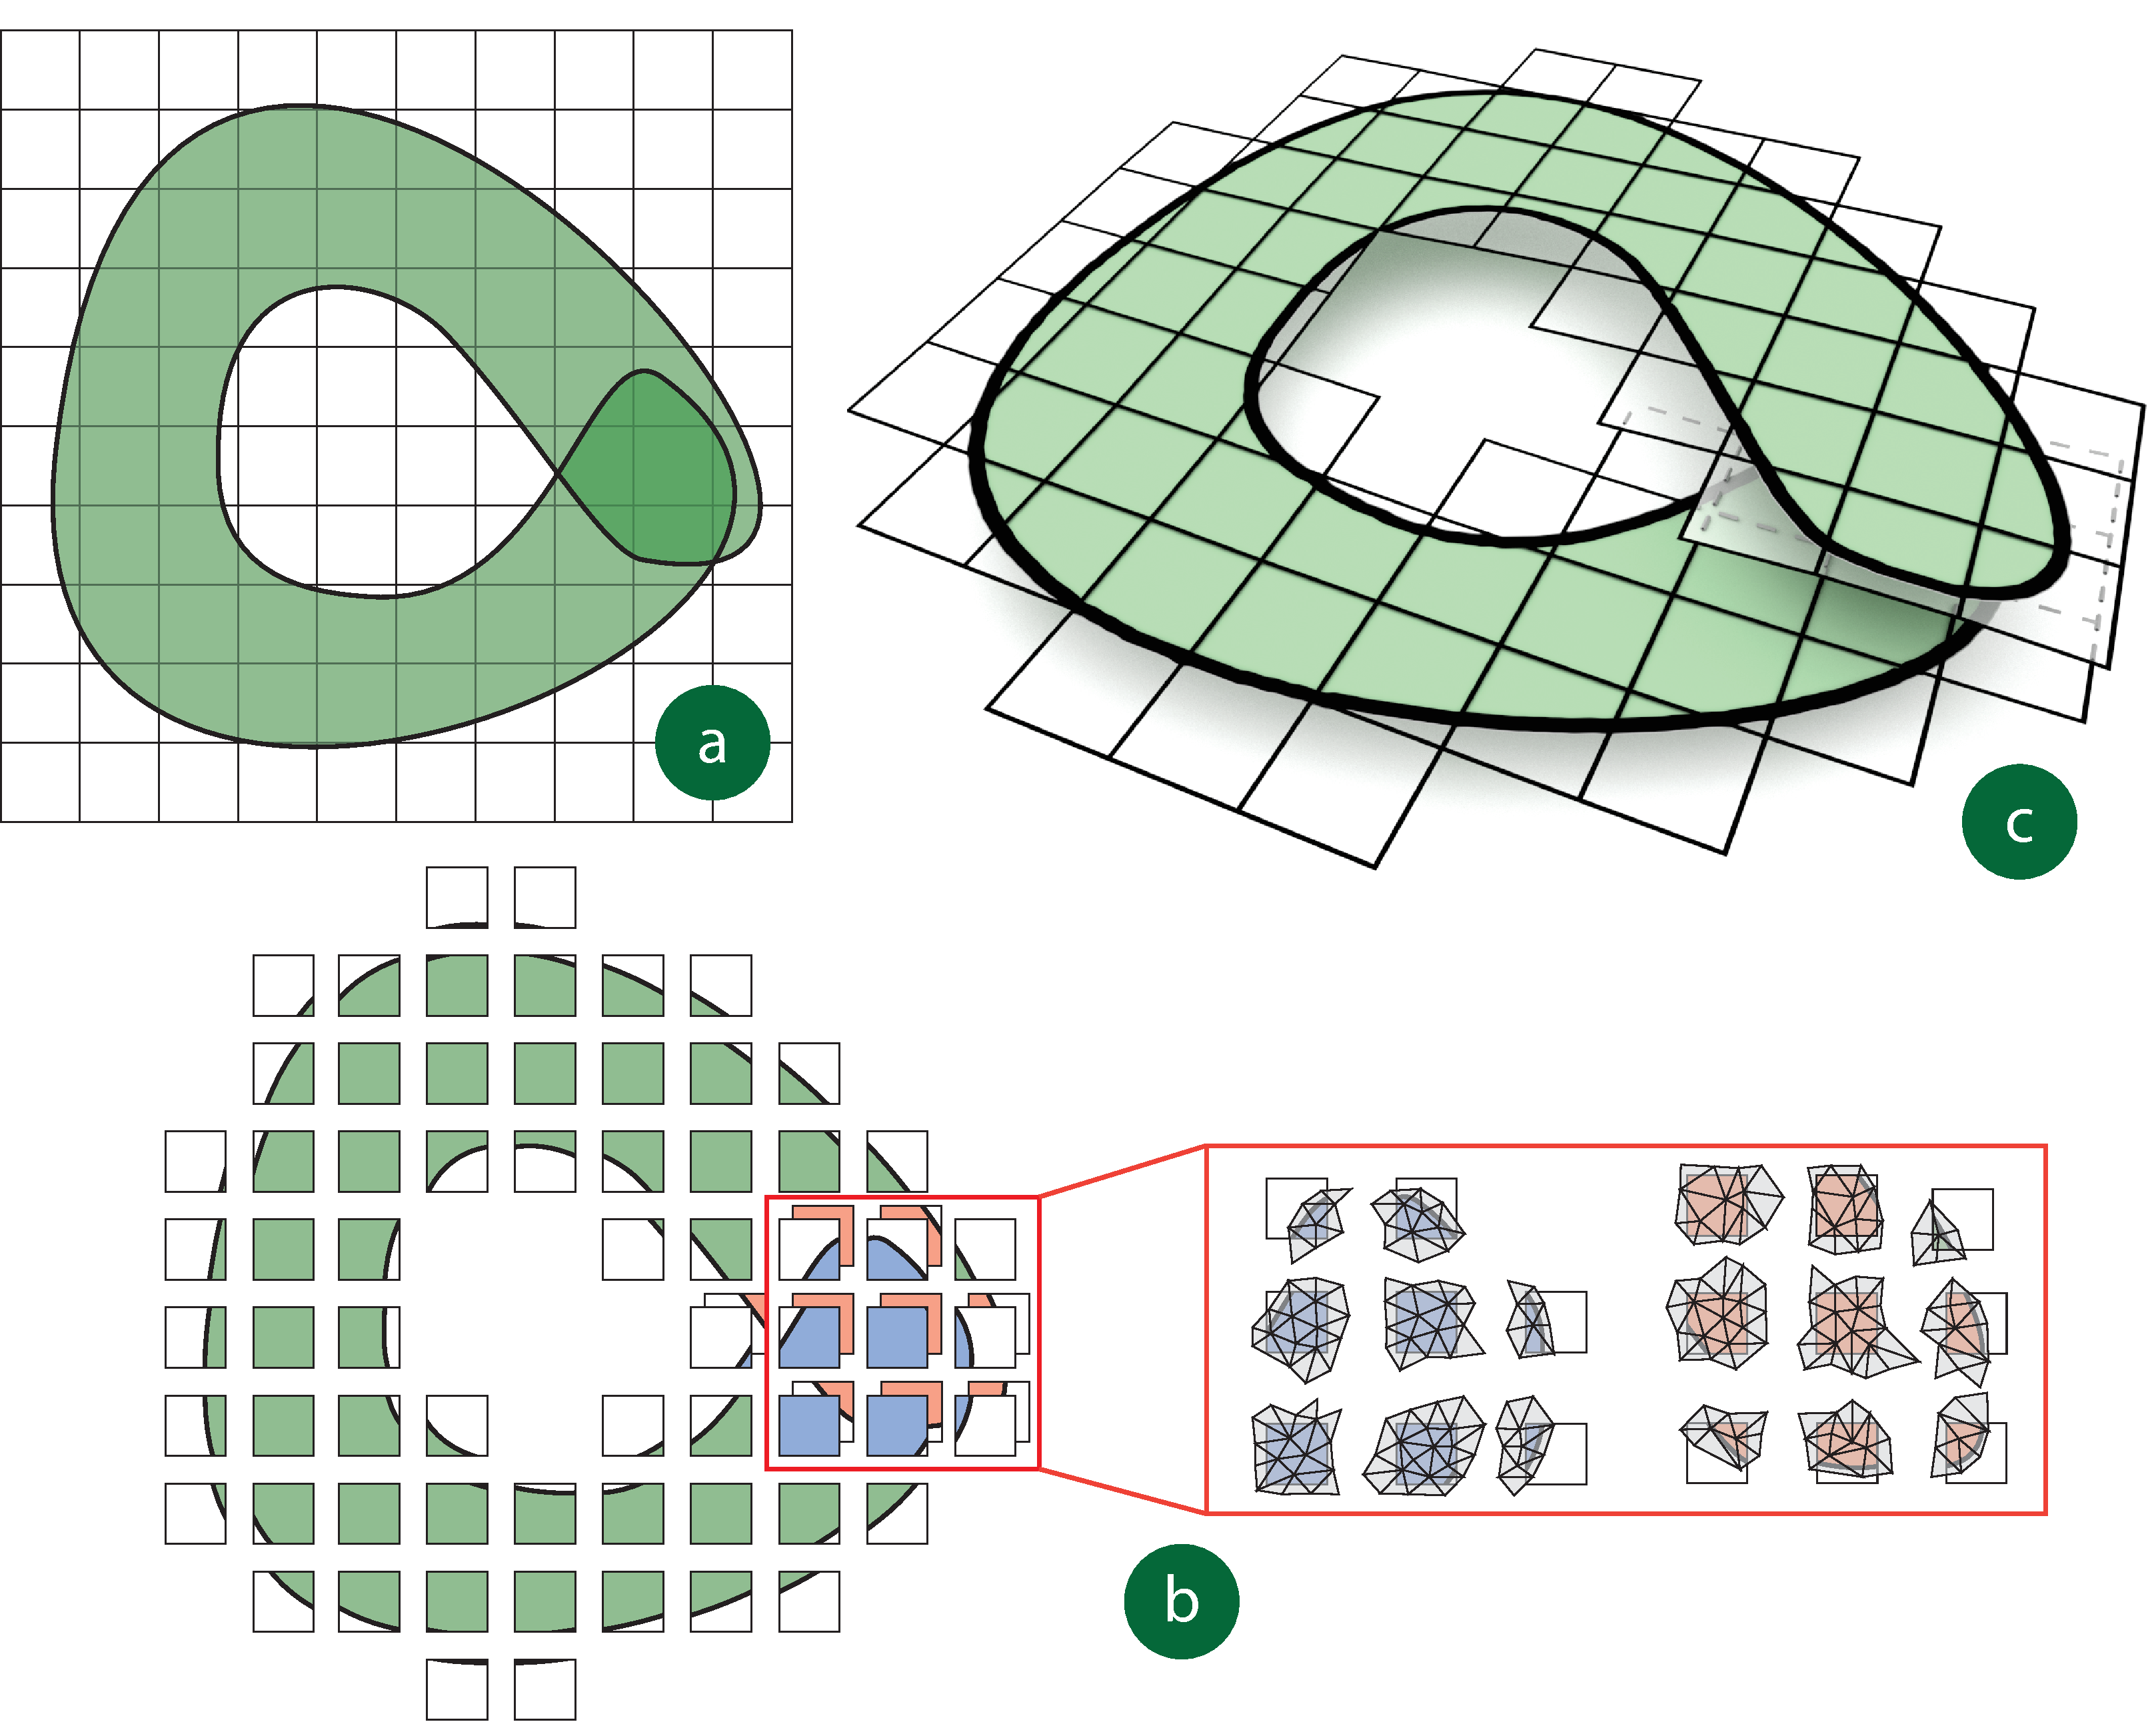
\includegraphics[width=.91\columnwidth]{chapter_nonmanifoldlevelsets/images/cshape_strip2.pdf}
\vspace*{-.1in}
\caption{Illustration of non-manifold mesh construction}{(a) A
  self-overlapping 2D model with template mesh overlaid. (b) Duplicate
  elements created during non-manifold embedded mesh generation, along
  with their associated material fragments. (c) Final non-manifold
  embedding mesh.  }
\label{fig:non-manifold-level-set-generation}
\vspace*{-.2in}
\end{figure}

Models such as the ones illustrated in Figure~\ref{fig:underresolved}
have been known to pose challenges not just for level set generation,
but also for certain dynamic simulation techniques even in the absence
of collision processing. Of course, simulation of elastic deformation
is a straightforward proposition, e.g.\ using the Finite Element
Method~\cite{SifakB:2012}, if an explicit tetrahedral mesh
representation of the model is available. However, if we wish to use
lattice deformer techniques, capable of high degrees of performance
optimization~\cite{RiverJ:2007,McAdaZSETTS:2011,MitchCS:2015}, we run
the risk of ``tying'' together disconnected material regions if they
are separated by a distance smaller than the embedding mesh resolution
(e.g.\ adjacent helices of the coil, or the two lips of the face model
pictured in Figure~\ref{fig:underresolved}). Fortunately, as we saw
earlier in this chapter, we have algorithms designed for constructing
embedding lattices capable of handling these thin incisions and fine
features. These methods add non-manifold connectivity to the embedding
mesh, duplicating elements and degrees of freedom as necessary to best
capture the embedded model topology.

\begin{figure}
  \centering
  \includegraphics[width=.8\columnwidth]{chapter_nonmanifoldlevelsets/images/TransitionFaceNew2.pdf}
\vspace*{-.1in}
  \caption{Illustration of handling material bifurcations}{(Left) An example where material bifurcates at an edge in a
    non-manifold Cartesian embedding. (Right) Level sets can only
    store a single interface transition at an edge. In the
    non-manifold level set bifurcations are explicitly recorded in
    \emph{transition faces} that record a connectivity graph between all cells on
    the left and right.}
\vspace*{-.2in}
  \label{fig:transition-face}
\end{figure}

Before discussing the details behind our non-manifold level sets, we
will take a moment to review a common formalism of the non-manifold
embedding process \cite{SifakDF:2007}. The algorithm is illustrated in
Figure~\ref{fig:non-manifold-level-set-generation}. This algorithm is
very similar to the one presented in Algorthim
\ref{alg:NonmanifoldMeshGeneration}, except here we are assuming a
material predicate defined by a triangulation (or tetrahedralization
in 3D). We do this partially to show how the algorithm adapts to
multiple material description predicates, but also to support models
with zero width cuts and overlapping geometry. These later aspects are
not supported by the discrete fine grid as presented earlier in the
chapter. The choice of material description is somewhat arbitrary - a
decision made around what geometric features one needs to capture. 

\textbf{Input:} (a) A geometric description of the shape to be
embedded (the green-shaded area in
Figure~\ref{fig:non-manifold-level-set-generation}). For simplicity,
we may assume the geometry is given as a triangulated model, which
allows us to express the self-overlap in our specific example. (b) A
mesh which will be used as a \emph{template} for our embedding
process. In Figure~\ref{fig:non-manifold-level-set-generation}(a) this
is the regular quadrilateral mesh pictured in the foreground.
\\
\textbf{Step 1 [Element separation]} We separate each element of the
template (quadrilateral) mesh, keeping track of the subset of our
material model that is contained in each such element (e.g.\ taking
note of all material triangles that intersected each quadrilateral).
\\
\textbf{Step 2 [Element duplication for disconnected components]} For
each embedding element, we identify all disjoint connected components
of material contained therein (e.g.\ by checking connectivity of the
respective material triangles). We generate a \emph{duplicate}
embedding (quadrilateral) element for each material component. Note
that, at this point, all embedding elements are still disconnected.
\\
\textbf{Step 3 [Restoring connectivity]} For any pair of
\emph{geometrically} adjacent embedding elements, we check if there is
material continuity across their common face (e.g.\ by checking if
they both intersect the same material triangle on that face). If such
continuity exists, we collapse all vertices along their common
face. This collapse is transitive; in the example of
Figure~\ref{fig:transition-face}(left) all three elements near a
convex material region have acquired a common face (with non-manifold
connectivity) due to transitive pair-wise vertex collapses.

The result is shown in Figure~\ref{fig:non-manifold-level-set-generation}(c); after discarding embedding elements with no material content, the final embedding
mesh has been fully assembled, with overlapping duplicates of elements properly connected, respecting the topology of the embedded material.

 
\begin{algorithm}
\caption{Non-Manifold Level Set Mesh Construction: This algorithm is a
modification of the procedure to generate a basic non-manifold
embedding (Algorithm \ref{alg:NonmanifoldMeshGeneration}) shown previously. The
modfications here account for the addition of transition faces to
track the interface near material bifurcations instead of simply
collapsing vertices greedily.}
\label{alg:NonmanifoldLevelsetMeshGeneration}
\begin{algorithmic}[1]
\Require Template Embedding Mesh $\mathcal{T}$, Material Description $\mathcal{M}$
\Procedure{Construct$\_$NonManifold$\_$LevelSet$\_$Mesh}{}
  \LineComment{Phase 1: Duplicate elements by connected components}
  \ForAll{Elements in $\mathcal{T}$ : $E_i$}
     \State $\mathcal{C}$ $\gets$ \Call{Connected$\_$Components}{$\mathcal{M}\cap E_i$}
     \ForAll{ Components in $\mathcal{C}$ : $m_j$ }
        \State $D_{i,j}$ $\gets$ \Call{Create$\_$Duplicate}{$T_i$ , $m_j$}
     \EndFor
  \EndFor
  \LineComment{Phase 2: Reconnect or build transition faces}
   \ForAll{Geometrically adjacent element pairs: $(E_k, E_l)$}
      \State  $\mathbf{G}$ $\gets$ \Call{Initialize$\_$Bipartite$\_$Graph}{$\mathcal{D}_{k}, \mathcal{D}_{l},\{\}$ }
      \ForAll{Duplicates from $E_k$ and $E_l$: $(D_{(k,q)}, D_{(l,r)})$}
         \If{
           \Call{Material$\_$Continuous}{$D_{(k,q)}$,$D_{(l,r)}$ } }
            \State \Call{Insert$\_$Edge}{$\mathbf{G},D_{(k,q)},D_{(l,r)}$}
         \EndIf
      \EndFor
      \ForAll{ Connected subgraphs of $\mathbf{G}$: $C_i$}
        \If{ $\#$\Call{Edges}{$C_i$} = 1 }
           \Comment Face is Manifold
           \State \Call{Collapse}{\textit{Vertices on common face}}
        \EndIf
        \If{ $\#$\Call{Edges}{$C_i$} $> 1$ }
           \Comment Face is Non-Manifold
           \State \Call{Register$\_$Transition$\_$Face}{$C_i$}
        \EndIf
      \EndFor
   \EndFor
\EndProcedure
\end{algorithmic}
\end{algorithm}

\subsection{Mesh bifurcation and transition faces}

The intent of our proposed level set data structure would be to store
signed distance values on the \emph{nodes} of the embedding mesh
produced by the algorithm just described (to our knowledge, these
\emph{non-manifold} embedding meshes have only been previously used to
store deformation data, not level set values). Of course, such signed
distances would be computed geodesically, along the embedding mesh,
rather than in the Euclidean sense. Subsequently, a continuous signed
distance field would be computed on the embedding mesh via standard
bilinear (2D) or trilinear (3D) interpolation. We note that in
``simple'' cases such as the example of
Figure~\ref{fig:non-manifold-level-set-generation} (where we have
element overlap, but no non-manifold connectivity) this approach would
have been fully sufficient. Unfortunately, scenarios such as the one
illustrated in Figure~\ref{fig:transition-face}(left) reveal a
newfound challenge: elements hinged in a non-manifold configuration on
a common face may disagree on the \emph{sign} of the signed distance
value stored on one of their common vertices. In
Figure~\ref{fig:transition-face}(left), elements \textsf{A1} and
\textsf{B2} record the vertex in orange as being inside the material
domain (hence carrying a negative level set value), while the same
vertex is outside the embedded domain (with a positive level set
value) as far as element \textsf{B1} is concerned. At this point, we
should emphasize that any discrete level set is an inherently
approximate representation of geometry, as it depends on interpolation
of signed distance value samples. The severity of this phenomenon,
however, is much greater as it carries the risk of eliminating parts
of the model boundary, or forcing it to spuriously appear in parts of
the embedding mesh that it did not originally traverse.  Note that
this behavior does not affect non-manifold embedding for simulation
purposes, since such techniques explicitly track the material embedded
in each element, rather than using interpolated vertices. 

\begin{figure}
  \centering
\subfloat{
\includegraphics[height=.2\paperheight]{chapter_nonmanifoldlevelsets/images/coil_001.png}
\hfill
\includegraphics[height=.2\paperheight]{chapter_nonmanifoldlevelsets/images/compression_001.png}
}
\subfloat{
\includegraphics[height=.2\paperheight]{chapter_nonmanifoldlevelsets/images/coil_040.png}
\hfill
\includegraphics[height=.2\paperheight]{chapter_nonmanifoldlevelsets/images/compression_005.png}
}
\subfloat{
\includegraphics[height=.2\paperheight]{chapter_nonmanifoldlevelsets/images/coil_065.png}
\hfill
\includegraphics[height=.2\paperheight]{chapter_nonmanifoldlevelsets/images/compression_020.png}
}
\subfloat{
\includegraphics[height=.2\paperheight]{chapter_nonmanifoldlevelsets/images/coil_100.png}
\hfill
\includegraphics[height=.2\paperheight]{chapter_nonmanifoldlevelsets/images/compression_060.png}
}

\vspace*{-.1in}
\caption{A non-manifold level set is used to correctly track
  self-collision of a coil}{(Top) A volumetric coil self-collides
  under user manipulation. (Bottom) A coil is compressed against two
  walls. Subsequently, collision handling is disabled and the geometry
  self-intersects (third frame in row). Self-collisions are turned
  back on and the coil recovers.}
\label{fig:coil}
\vspace*{-.15in}
\end{figure}


We posit that, for the proper resolution of non-manifold connectivity,
the Algorithm \ref{alg:NonmanifoldMeshGeneration} presented in 
Section~\ref{sec:nonmanifoldmeshgeneration} and
Section~\ref{sec:stockembedding} cannot be allowed to
indiscriminately collapse vertices (in Step 3) based solely on
material continuity, if this yields a contradiction in the nodal
signed distance values across connected elements. Thus, we introduce
the concept of a \emph{transition face} which encodes connectivity
between incompatible (in terms of the signs of nodal distance values)
materially connected elements. This construct is illustrated in Figure
~\ref{fig:transition-face}(right). The transition face is envisioned
as an infinitesimally thin connective strip between between elements
\textsf{A1}, \textsf{B1} and \textsf{B2} with the appropriate internal
structure as to connect the material of each element \emph{as
  reconstructed from their nodal values} via bilinear
interpolation. For example, we see that element \textsf{A1} is
considered to be fully interior to the domain, once described by the
signed distance values stored at its nodes. We explicitly
  store a transition face as a \emph{connected} bipartite
graph as seen in Figure~\ref{fig:transition-face}, which
records pairwise material continuity of elements on
either side, which would normally be lost once only nodal level set
values are retained for each element.

\subsection{Non-manifold level set mesh algorithm}


Using the transition face mechanism, we can now describe our new
algorithm for generating the embedded mesh whose nodes will be used to
store the signed distance values of our non-manifold level set. The
entire process is outlined in Algorithm
\ref{alg:NonmanifoldLevelsetMeshGeneration}. The first phase of the
algorithm is identical to the initial phase of the stock embedding
algorithm \ref{alg:NonmanifoldMeshGeneration}. As before, given a
geometric material description $\mathcal{M}$ (e.g.\ a tessellation of
the model) we identify the material region $\mathcal{M}\cap E_i$
contained within the embedding element $E_i$ from an embedding
``template'' mesh $\mathcal{T}$. We identify connected components
$\{m_j\}_j$ in this set, and create a duplicate embedding element
$D_{i,j}$ associated with each material component. As before, all
duplicate elements $D_{i,j}$ are completely disconnected at this
point.

Subsequently, we analyze material continuity on adjacent embedding
elements, with the goal of reconnecting the previously separated
elements into the final embedding mesh. For any two elements $E_k$,
$E_l$ that were adjacent in the template mesh $\mathcal{T}$, we
identify the sets $\mathcal{D}_k=\{D_{k,q}\}_q$ and
$\mathcal{D}_l=\{D_{l,r}\}_r$ of duplicate elements that were
respectively spawned from them. We examine each possible pair
$(D_{k,q}, D_{l,r})$ drawn from these sets for material continuity
across their common face. At this point, however, instead of
collapsing vertices on the common face of such pairs that are found to
be materially connected, we simply record this connectivity with an
edge in a bipartite graph $\mathbf{G}$ defined over the sets
$\mathcal{D}_k$ and $\mathcal{D}_l$. Once all pairs from
$\mathcal{D}_k$ and $\mathcal{D}_l$ have been processed, we proceed to
split the graph $\mathbf{G}$ into its connected components (in terms
of graph connectivity, not\changed{ material connectivity as}{ to be
  confused with the connected components of material} in Phase 1). For
every connected component (subgraph) of $\mathbf{G}$, we proceed as
follows:
\begin{itemize}
\vspace*{-.08in}
\item If a connected subgraph contains \emph{exactly} one edge, the
  duplicate elements $D_{k,q}$ and $D_{l,r}$ connected by that edge
  are guaranteed to be compatible relative to the sign of the distance
  value stored on their nodes, since they agree exactly on the
  material intersecting their (geometrically) common face. This is a
  consequence of this edge being a connected component of
  $\mathbf{G}$, indicating that no other element is independently
  connected to either $D_{k,q}$ or $D_{l,r}$. In this case, we are
  free to collapse the vertices of the two duplicate elements across
  their common face, exactly as we did in
  section~\ref{sec:stockembedding}.  \vspace*{-.08in}
\item If a connected subgraph contains two or more edges (see
  Figure~\ref{fig:transition-face}(right)), we cannot collapse all
  vertices on the duplicate elements' common face, since some of these
  elements may disagree on the sign of the distance field stored on
  their nodes. In this case, we simply generate a transition face,
  which is encoded using the same connected subgraph, allowing the
  duplicate elements that are juxtaposed on that transition face to
  retain independent signed distance values on their nodes.  As we
  will see in the next sections, a transition face is semantically
  equivalent to a ``hard'' topological connection (a collapsed face)
  for operations that traverse the final embedding mesh, with the
  exception of its ability to allow separate signed distance values on
  each duplicate element it connects.
\end{itemize}
\vspace*{-.08in}

% \textbf{Implementation notes} We have thus far assumed that the
% material model $\mathcal{M}$ is given as an explicitly meshed object
% (e.g.\ a tetrahedralized volume in 3D). However, this is not strictly
% necessary and \emph{any} material description that can answer the
% predicates of Algorithm 1, lines 4 (connectivity within an element)
% and 11 (material continuity across elements) can be trivially used in
% the same framework.

For example, Figure~\ref{fig:zero-width} demonstrates an elastic model
being cut by a user-specified fracture surface. For this, we leveraged
the method of Sifakis et al.~\shortcite{SifakDF:2007} which explicitly
subdivides each element of the template mesh $\mathcal{T}$ into
disjoint polyhedra (a 2D analogue of this process is shown in the
inset image to the right, where a ``cutting curve'' of line segments
is used to section square cells into polygonal regions). This
decomposition natively provides connectivity information, and can
easily detect material continuity across embedding elements by
checking adjacency of polyhedral material regions.  Finally, the
transitive \textsf{Collapse} operation (line 15) is simply implemented
using a \textsf{Union-Find} structure which records the equivalences
of vertex identifiers.



\begin{figure}
  \centering
\includegraphics[width=.46\columnwidth]{chapter_nonmanifoldlevelsets/images/ball_drop_zero_width_030.png}
\includegraphics[width=.46\columnwidth]{chapter_nonmanifoldlevelsets/images/ball_drop_zero_width_040.png}
\includegraphics[width=.46\columnwidth]{chapter_nonmanifoldlevelsets/images/ball_drop_zero_width_100.png}
\includegraphics[width=.46\columnwidth]{chapter_nonmanifoldlevelsets/images/ball_drop_zero_width_160.png}
\vspace*{-.1in}
\caption{Non-manifold level sets can correctly handle zero width cuts}{A cube is partially sliced by 6 planes and a ball
  subsequently squashes it to push the resulting 16 fingers apart. Our
  non-manifold level set can robustly resolve zero width cuts which
  could not be resolved with standard Cartesian grid-based level sets.}
\label{fig:zero-width}
\vspace*{-.2in}
\end{figure}



\subsection{Level set operations on nonmanifold meshes}


%\vspace*{-.06in}
\paragraph{Initialization of signed distances} Once the topology of
the embedding mesh has been constructed, including the creation of the
necessary transition faces, the embedding mesh nodes must be populated
with the proper signed distance values. We start by explicitly
computing such distances on embedding elements that intersect the
object boundary. Since we possess an explicit description of the
material contained in each element, for each of their nodes we compute
the minimum (absolute) distance from all material contained in that
element. We also compute the sign depending on whether the node is
inside or outside the embedded material component. Adjoining elements
that have had common vertices collapsed (topologically; not connected
via transition faces) will agree on the sign of the signed distance
field at shared nodes, but not necessarily the magnitude. We retain
the distance value with the \emph{minimum} magnitude, across all
elements incident to this node. Of course, no such reduction is
performed on nodes connected via transition faces. Subsequently, we
propagate the signed distance field in the interior of the object
using the $O(n\log n)$ Fast Marching Method~\cite{Sethi:1998}, with
the only modification that this Dijkstra-type algorithm is allowed to
propagate through transition faces in exactly the same fashion as
through explicitly connected nodes.  While we only compute a scalar
signed distance field, it would be straightforward to also compute a
normal field \cite{KobbeBSS:2001} to support higher quality
reconstructions.

\begin{figure}
\vspace*{-.2in}
\centering
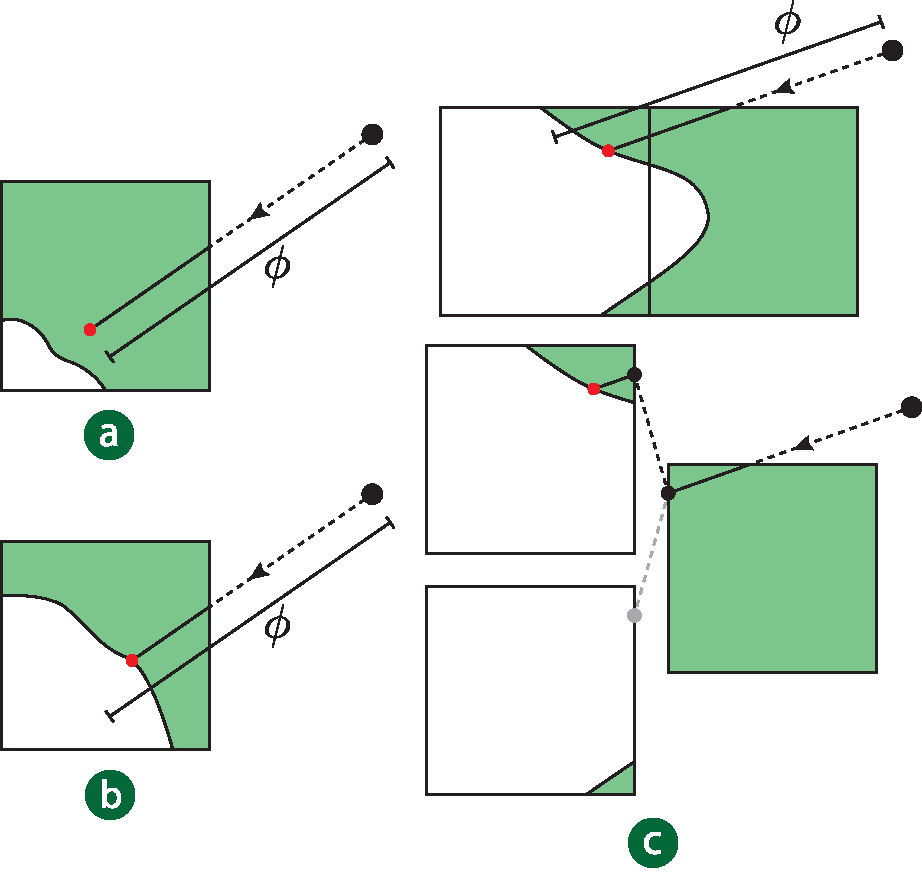
\includegraphics[width=.88\columnwidth]{chapter_nonmanifoldlevelsets/images/backtrace-cases-alternative-4.pdf}
\vspace*{-.1in}
\caption{Illustration of the backtrace procedure to determine surface crossings}{Different surface projection scenarios. (a) Backtracing terminates after covering a distance of $\phi$ without intersecting the interface. (b) Backtracing stops at the
  first interface crossing. (c) Backtracing hits a transition
  face and continues into the connected neighbor that has the negative $\phi$
  value with the smallest magnitude.}
\label{fig:backtrace}
\end{figure}



\vspace*{-.12in}
\paragraph{Distance queries and surface projection} The basic level
set predicates required in the collision pipeline of section
\ref{sec:self-collisions} include a lookup of the signed distance
value $\phi(\vec{x})$ at an arbitrary location $\vec{x}$ in space, and
the projection of a material point to the closest location
$\textsf{Proj}(\vec{x};\Gamma)$ on the model surface $\Gamma$. Since
our embedding mesh may contain several overlapping elements, it is no
longer sufficient to define such predicates as functions of just the
spatial location $\vec{x}$ being queried; we also need to identify the
appropriate branch of material being referred to. Thus, we reformulate
these predicates as $\phi(\vec{x},D_i)$ and
$\textsf{Proj}(\{\vec{x},D_i\};\Gamma)$, where the element $D_i$
embeds the material point $\vec{x}$ in the non-manifold level set
mesh. Subsequently, the result of the projection operator is also a
tuple $(\vec{x}^\star,D_j)$ denoting a material point $\vec{x}^\star$
and its respective embedding element $D_j$.


\begin{figure}
\centering
\subfloat{
\includegraphics[width=.4\columnwidth]{chapter_nonmanifoldlevelsets/images/zplasty_001.png}
\hfill
\includegraphics[width=.4\columnwidth]{chapter_nonmanifoldlevelsets/images/net_000.png}

}
\subfloat{
\includegraphics[width=.4\columnwidth]{chapter_nonmanifoldlevelsets/images/zplasty_050.png}
\hfill
\includegraphics[width=.4\columnwidth]{chapter_nonmanifoldlevelsets/images/net_030.png}
}
\subfloat{
\includegraphics[width=.4\columnwidth]{chapter_nonmanifoldlevelsets/images/zplasty_090.png}
\hfill
\includegraphics[width=.4\columnwidth]{chapter_nonmanifoldlevelsets/images/net_050.png}
}
\subfloat{
\includegraphics[width=.4\columnwidth]{chapter_nonmanifoldlevelsets/images/zplasty_540.png}
\hfill
\includegraphics[width=.4\columnwidth]{chapter_nonmanifoldlevelsets/images/net_110.png}
}
\caption{Non-manifold level sets handle surgical scenarios and complex
  woven geometry}{(Left) Surgical simulation of a z-plasty procedure,
  with self-collision processing. (Right) A net is stretched out,
  twisted to a saddle configuration and a ball is subsequently dropped
  on it. A single level set is used for the entire net during
  self-collision processing.}
\label{fig:zplasty-and-net}
\end{figure}


Given an embedding element $D_l$ and a location $\vec{x}$ embedded in it, level set value and gradient are computed via trilinear interpolation:

$$
\phi(\vec{x},D_l)=\!\!\!\!\sum_{i,j,k=0}^1\!\!\!\mathcal N_{ijk}(\vec{x})\phi_{ijk},\ \ 
\nabla\phi(\vec{x},D_l)=\!\!\!\!\sum_{i,j,k=0}^1\!\!\!\mathcal \nabla\mathcal N_{ijk}(\vec{x})\phi_{ijk}
$$
where $\mathcal N_{ijk}$ denotes the trilinear basis functions and
$\phi_{ijk}$ are the signed distance values at the nodes of $D_l$.
This formula for the gradient can be used throughout the embedding
mesh, and has been fully adequate for our collision processing
application. However, should higher accuracy be desired, a higher
order finite difference scheme~\cite{OsherF:2002} can be optionally
substituted for cells exibiting manifold connectivity with all their
neighbors.  It is known that the gradient of the level set function,
i.e.\ the steepest ascent direction of the distance field, is a unit
normal which points in the direction of the closest point on the
surface. Thus, the closest point to $\vec{x}$ on the model surface is
to be found in the direction of $\vec{n}=\nabla\phi(\vec{x},D_l)$, at
a distance of $|\phi(\vec{x},D_l)|$. Thus, analytically:

\vspace*{-.08in}
$$
\textsf{Proj}(\{\vec{x},D_l\})=\vec{x}-\phi(\vec{x},D_l)\nabla\phi(\vec{x},D_l)
$$


To compute the projection
$\textsf{Proj(}\{\vec{x},D_l\};\Gamma\textsf{)}$ we topologically
backtrace the non-manifold level set mesh along $\vec{n}$
element-by-element, to ensure that we follow a geodesic path along the
embedding mesh, as shown in Figure~\ref{fig:backtrace}. If while
traversing a distance $\phi(\vec{x},D_l)$ along $\vec{n}$ we land in
an element $D_m$ that is crossed by the interface, then we use
bisection search to compute the interface point $\vec{x}^\star$ and
return the tuple $(\vec{x}^\star,D_m)$
(Figure~\ref{fig:backtrace}(b)). If we have traversed a distance equal
to $\phi(\vec{x},D_l)$ without crossing any interface, we stop the
backtrace operation and report the location reached after the
requisite distance has been traveled (Figure~\ref{fig:backtrace}(a));
we do so to avoid grazing by a nearby interface without actually
stopping there. Finally, if the backtracing process crosses a
transition face $f$, then we compute the point $\vec{x}_f$ where the
ray from $\vec{x}$ along $\vec{n}$ crosses $f$. We then compute the
value of $\phi$ at $\vec{x}_f$ for all elements on the other side
(connected through the transition face) and choose the one with a
\emph{negative} value but with the \emph{minimum} magnitude (to
approach the surface as soon as possible). If no such element is
present, then we assume that the interface lies \emph{exactly} at
$\vec{x}_f$ and return this point along with the cell from which we
entered the transition face as the result of the projection. We note
that although this projection is approximate, the error is comparable
with conventional, grid-based level sets, and perfectly acceptable for
our collision handling scheme.




\vspace*{-.02in}
\section{Examples}
\label{sec:examples}
\vspace*{-.03in}

We simulated a number of examples to demonstrate the efficacy of our
method in several challenging scenarios.
%
Figure~\ref{fig:coil}(top) shows a user pulling a three dimensional
volumetric coil at the red handle creating complex
self-collisions. Figure~\ref{fig:coil}(bottom) shows the same coil
being compressed against two moving walls. Self-collisions are turned
off at some point to make the geometry self-intersecting, and
subsequently turned back on again resulting in the coil bulging
outwards. This example shows that our method does not require any
history information for resolving self-collisions.
%
Figure~\ref{fig:zplasty-and-net}(top) shows a simulation of a common
maneuver in plastic surgery, called a \emph{Z-plasty}, while
Figure~\ref{fig:zplasty-and-net}(bottom) shows a ball dropping on a
net that has been stretched outwards and twisted into a saddle
configuration. Our method uses a single level set for the entire net
during self-collision processing, obviating the need for multiple
collision level sets and circumventing the complexity in bookkeeping
associated with such scenarios.
%
Figure~\ref{fig:face}(b) shows an example where the lower jaw of a
face model is pulled down and subsequently pushed back up, opening and
closing the mouth in the process. Note the slight bulge in the cheeks
due to self-collisions at the lips when the mouth is closed because
the jaw is pushed further up compared to the rest state.
Figure~\ref{fig:face}(c) shows a user moving around two points on the
lips (shown in orange) to demonstrate complex self-collisions that our
method can resolve.
%
Finally, Figure~\ref{fig:zero-width} shows an example where a cube is
partially sliced by six planes using the method
of~\cite{SifakDF:2007}. This results in sixteen fingers which are
pushed apart when squashed by a ball from the top. Note that a
standard Cartesian grid-based level set cannot be used for resolving
this structure irrespective of its resolution.



\renewcommand{\arraystretch}{.8}
\setlength{\tabcolsep}{3pt}


\begin{table}[h!]
\begin{center}
\setlength\fboxsep{0pt}
\setlength\fboxrule{0.25pt}
\sffamily
\begin{tabular}{
 >{}l
 >{}m{2cm}
 >{}l 
 >{}m{2cm} 
 >{}m{2cm} 
 >{}m{1cm} }
\toprule
\textbf{Model}& \textbf{Level\;set Gen.\,(s)} & \textbf{Solve\,(s)} & \textbf{Collision Proc.\,(s)} & \textbf{Backtrace Total\,(ms)} & \textbf{Proxy Count}\\
\midrule
\textbf{Z-plasty}& 222.6 &  1.961 & 0.0671 & 0.0479 & 7121\\
\midrule
\textbf{Coil}& 580.5 & 13.22 & 0.4651 & 14.8 & 31126\\
\midrule
\textbf{Net}& 524.0 & 23.47 & 0.4123 & 5.38 & 48042\\
\midrule
\textbf{Face}& 271.0 & 24.46 & 0.2977 & 0.620 & 48851\\
\bottomrule
\end{tabular}
\end{center}
\vspace*{-.1in}
\caption{Performance results for non-manifold level set generation and
  collision processing}{Example timing comparing the cost of solving
  elasticity equations to running collision detection using our
  non-manifold level set data structure. Compared to the cost of
  simulation per frame, collision processing is generally
  insignificant. Level set generation, while currently expensive,
  is performed only as a pre-processing step.}
\label{tab:compute-times}
\end{table}


This table captures the performance impact of our collision
methodology. The first column lists the computation times for
generating the non-manifold level set mesh; we emphasize that this is
a one-time precomputation cost, before dynamic simulation even
starts. The following columns list the cost for each step of our
Backward Euler implicit integration scheme, divided into the solution
of the linearized equations, the cost of collision processing, and
specifically the aggregate cost of all backtracing operations for
projecting proxies to the object surface. It can be seen that the cost
of collision processing is a minute fraction of the overall
simulation. This stems from the fact that we do not require a history
of collision-free states, and can take more aggressive steps than
semi-implicit schemes that disallow
interpenetration~\cite{BridsFA:2002}.


\begin{figure}
  \centering
\includegraphics[width=.91\textwidth]{chapter_nonmanifoldlevelsets/images/face-strip.pdf}
\vspace*{-.1in}
\caption{Non-manifold level sets are applicable to simulating small
  facial features}{(a) Cutaway view of the non-manifold level set
  generated on a face model. (b) The lower jaw is displaced
  vertically, opening and closing the mouth. Note the small bulges in
  the cheek due to self-collisions at the lips because the jaw is
  pushed further up compared to the rest state.  (c) A user moves
  around two points on the lips (orange) to demonstrate the robustness
  of our method in resolving self-collisions. }
\label{fig:face}
\vspace*{-.15in}
\end{figure}




%%% Local Variables:
%%% mode: latex
%%% TeX-master: "../document"
%%% End:

\chapter{Parallelization Techniques for Lattice Deformers}
\label{chp:parallelization}

In this chapter, we will explore techniques for optimizing the force
computation procedures for lattice deformers. Recall from Chapter
\ref{chp:engineering}, that our goal in solving elastic deformations
is to compute forces and force differentials from current nodal
positions. We codified this process in Algorithm
\ref{alg:isotropicforces}, where we detailed the computational steps
required for converting nodal positions into the corresponding nodal
forces according to a material specific energy function. The important
take away from this algorithm is that we are able to compute these
forces on a per cell basis. On the surface, this would seem to be an
excellent opportunity for thread-based parallelism: divide all the
cells among available processor cores and have each core operate on
its cells in isolation. Unfortunately, this is where we run into
problems.

The first problem is that while all cells are functionally
independent, the nodes themselves are not. When we compute forces on
nodes, we are actually producing aggregate forces. That is, for any
node in the lattice, we are interested in sum of all forces from all
cells it is connected with. By using thread-based parallelism, we
encounter a significant problem.  In the context of a single thread,
the processing of cells is serial. But when two or more threads, each
operating on different cells, try to accumulate to a single node we
encounter a serious \textit{write hazard}. In this case, the hazard is
that we don't have any guarantees that our final result will be the
sum of all forces from all involved cells. Due to the behaviors of the
processor caches and system memory, we might have a result equal to
any one single cell's result, any combination of the cells combined,
or some unrelated value. We could attempt to remove this confusion by
adding a locking protocol around each node, but this would introduce
significant performance penalties.

The second problem we encounter is when reading and writing nodal
information. In Chapter \ref{chp:nonmanifold}, we demonstrated how
non-manifold embedding meshes could be constructed to represent
material geometry with thin features or incisions. However, this
approach comes with a significant drawback: The explicit topology
required to define the mesh removes much of the regularity we could
otherwise depend on for performance. One nice benefit of using an
implicit topology for our lattices is that the memory locations of all
cells and nodes can be quickly computed via a function of their
geometric positions. This allows reading and writing to these
locations to be done via a single memory access: the exact storage
location. In contrast, the explicit topology we constructed
previously has no such guaranteed relationship between storage
locations and geometric positions. Instead it uses an explicit record
of pointers for each cell that informs us where the memory is
stored. This can hurt performance in two ways: first, there is no
guarantee that memory is well ordered. Neighboring geometric nodes
might be arbitrarily far apart in memory. Since modern processors load memory in
linear strips, known as cache lines, this distance might require
multiple loads, where a single load might have sufficed if they were
closer. Second, by using a collection of pointers per cell, we are
actually reading twice for every entry. The first read is to load the
value of the pointer, followed by the data itself. Combined, these
memory access issues can be extremely detrimental to performance,
especially since modern processors operate in a regime of roughly two
orders of magnitude more available computational resources than memory
access rate. Despite the significant number of numerical steps
required to process each cell, any delays in memory access could lead
to the computation becoming memory bound.

We can deal with these problems by more carefully arranging our data
for computation. Our proposed solution makes use of two concepts:
hybrid grids and blocking. Along the way, we will also show how C++
templates can be employed for guiding SIMD vectorization of
blocks. The following sections will cover these concepts in more detail.

\section{A hybrid embedding lattice structure}
\label{sec:hybrid}

We build on the non-manifold embedding mesh concepts discussed in
Chapter \ref{chp:nonmanifold}, but now we seek to optimize these
data structures for computational performance. Although the use of
non-manifold embedding meshes recovers much of the topological
expressive ability of conforming meshes, it jeopardizes one of the
most attractive features of regular embedding lattices, the fact that
connectivity is implicit in the lattice structure as opposed to
explicitly stored in a mesh. The performance impact of implicitly
defined topology can be profound; the memory footprint of explicitly
stored connectivity information can easily exceed the state variables
themselves (e.g. nodal positions) and reduce effective memory
bandwidth by necessitating indirect memory access. In this section, we
strive to leverage the best of both worlds: We use an (implicit
topology) Cartesian grid to capture the majority of the embedded model
in regions where non-manifold duplication is not needed. We retain the
topological flexibility of non-manifold embedding lattices by
hybridizing this grid with an (explicit topology) hexahedral mesh used
to describe regions in the vicinity of narrow slits and incisions.


% \begin{figure}
% \centering
% \subfloat{
% \includegraphics[height=.2\paperheight]{chapter_gridiron/example_images/Single_zPlasty_1/embedded/render0057.png}
% \hfill
% \includegraphics[height=.2\paperheight]{chapter_gridiron/example_images/Rhomboid_Scalp_1/embedded/render0010.png}
% }

% \subfloat{
% \includegraphics[height=.2\paperheight]{chapter_gridiron/example_images/Single_zPlasty_1/embedded/render0071.png}
% \hfill
% \includegraphics[height=.2\paperheight]{chapter_gridiron/example_images/Rhomboid_Scalp_1/embedded/render0022.png}
% }

% \subfloat{
% \includegraphics[height=.2\paperheight]{chapter_gridiron/example_images/Single_zPlasty_1/embedded/render0093.png}
% \hfill
% \includegraphics[height=.2\paperheight]{chapter_gridiron/example_images/Rhomboid_Scalp_1/embedded/render0046.png}
% }

% \subfloat{
% \includegraphics[height=.2\paperheight]{chapter_gridiron/example_images/Single_zPlasty_1/lattice/render0071.png}
% \hfill
% \includegraphics[height=.2\paperheight]{chapter_gridiron/example_images/Rhomboid_Scalp_1/lattice/render0022.png}
% }

% \vspace*{-.08in}
% \caption{Simulation of Z-Plasty and Rhomboid flap repairs}{Left:
%   Simulation of \textbf{Z-Plasty}, a basic maneuver resulting in
%   anisotropic scaling along two perpendicular directions. Z-Plasty is
%   a common building block leveraged in more elaborate repairs. Right:
%   \textbf{Rhomboid flap} procedure for closing a quadrilateral
%   aperture of excised tissue on the scalp. The embedded simulation
%   grids are shown on the right.}
% \label{fig:Zplasty-RhomboidScalp}
% \vspace*{-.16in}
% \end{figure}


% \begin{figure}
% \centering
% \subfloat{
%  \includegraphics[width=.35\paperwidth]{chapter_gridiron/example_images/Dual_sPlasty_Scalp_1/embedded/render0023.png}
% \hfill
% \includegraphics[width=.35\paperwidth]{chapter_gridiron/example_images/Dual_sPlasty_Scalp_1/embedded/render0066.png}
% }

% \subfloat{
% \includegraphics[width=.35\paperwidth]{chapter_gridiron/example_images/Dual_sPlasty_Scalp_1/embedded/render0115.png}
% \hfill
% \includegraphics[width=.35\paperwidth]{chapter_gridiron/example_images/Dual_sPlasty_Scalp_1/lattice/render0066.png}
% }
% \vspace*{-.1in}
% \caption{Simulation of a Dual S-Plasty repair on the scalp}{\textbf{Dual S-Plasty} procedure on the scalp; a large oval-shape defect is patched by transposing two S-shaped flaps.}
% \label{fig:SPlasty-Scalp}
% \vspace*{-.15in}
% \end{figure}

\subsection{Reduction and Remapping}

To transform an explicit non-manifold mesh into a hybrid grid, we
attempt to map as much of the explicit-connectivity mesh as possible
back onto an implicit-connectivity grid to recover regularity. From
the explicit mesh, we have two geometric primitives to consider for
remapping: nodes and cells. For simplicity, we will first consider
nodes and then cells. Figure \ref{fig:remapping} illustrates the
results of the remapping rules below:
\begin{itemize}
\vspace*{-.05in}\item Nodes are mapped to the grid if and only if they possess no duplicates.
\vspace*{-.05in}\item Cells are mapped to the grid if and only if all of their vertices have been mapped to the grid.
\end{itemize}
\vspace*{-.05in} Each mesh cell remaining in the hybrid lattice is
associated with a coordinate from the grid. This mapping will become
important later when we discuss the block-based acceleration
structures.  After these rules are applied, the new structure must
adhere to several post-conditions.
\begin{itemize}
\vspace*{-.05in}\item All grid cells are composed only of grid nodes.
\vspace*{-.05in}\item Mesh cells contain one or more mesh nodes.
\end{itemize}
It should be noted that this set of rules is not strictly optimal in
the sense of mapping the most elements into the grid. A more
aggressive strategy would be to select one element from each set of
geometrically co-located items and map it to the grid. We defer
investigation of similar compaction heuristics to future work.
\textbf{Note:} In these surgical examples (Figure \ref{fig:surgicalembeddings}) mesh-mapped embedding cells are indicated
with blue color, grid-mapped ones in red. Typically, only a minority
of cells is mesh-mapped, allowing us to retain the bulk of performance
benefits of implicit grid-mapped embeddings.


\begin{figure}
  \centering
\vspace*{-.12in}
  \includegraphics[width=3in]{chapter_gridiron/images/Figure_Topology_D}
\vspace*{-.07in}
  \caption{Illustration of cell type categorization}{From an explicit mesh (top), we generate (a) mesh mapped nodes in red, grid mapped nodes in black and (b) mesh mapped cells in red, grid mapped cells in gray.}
  \label{fig:remapping}
\end{figure}

\begin{figure}
  \centering
  \includegraphics[width=.32\paperwidth]{chapter_gridiron/example_images/Dual_sPlasty_Scalp_1/lattice/render0066.png}
  \includegraphics[width=.32\paperwidth]{chapter_gridiron/example_images/Single_zPlasty_1/lattice/render0071.png}
  \includegraphics[width=.32\paperwidth]{chapter_gridiron/example_images/Rhomboid_Scalp_1/lattice/render0022.png}
  \caption{Embedding discretizations of surgical operations}{Three
    different surgical operations, S-Plasty (Top Left), Z-Plasty (Top
    Right), and a Rhomboid Flap (Bottom), are shown with their
    embedding hybrid grids. Cells in red are part of the grid region, while
    blue cells are mesh mapped. Green cells mark Dirichlet regions.}
  \label{fig:surgicalembeddings}
\end{figure}

\section{Parallelization}

\begin{algorithm}
  \caption{General Parallelization Design Strategy}
  \label{alg:GeneralStrategy}
  \begin{algorithmic}[1]

    \For{ $t = 0 \ldots N$ }

    \State $\{ o_1(t), o_2(t),\ldots, o_m(t) \} = \Call{Kernel}{\{ i_1(t), i_2(t),\ldots, i_n(t) \}}$
    
    \EndFor
    
  \end{algorithmic}
  
\end{algorithm}


Our framework relies on both multithreading and vectorization (SIMD)
to obtain the best possible performance. The fact that our
Cartesian-based discretization consists of identically shaped elements
offers a great opportunity to leverage both thread-level and
data-level parallelism, due to the inherent regularity of the
simulation kernels. Our general strategy is to design operations that
resemble the form shown in Algorithm \ref{alg:GeneralStrategy}. Under
this approach, our numerical kernels for computing nodal values
operate on multiple streams of input data,
$\{ i_1, i_2,\ldots, i_n \}$, and produce multiple streams of output
data, $\{ o_1, o_2,\ldots, o_m \}$. Collections of streams can be
grouped together logically into vectors or matricies. By structuring
the computation in this form, we can clearly see where multithreading
and vectorization apply: Each thread will be assigned a partition over
$N$, while vectorization can be used to execute multiple instances of
\textsc{Kernel} by stepping through the partition in strides. This
also suggests a data structure design: Arrays of Structs of Arrays
(AoSoA), where each struct contains the data for each computational
stride and the array of structs can be divided evenly between
threads. In the next couple of sections, we will look at how the
simulation data, currently arranged in a hybrid grid, can be
repackaged according to the AoSoA methodology, a process called blocking. 

\begin{algorithm}
\caption{SIMD Compatible Block Construction}
\label{alg:BlockGeneration}
\begin{algorithmic}[1]
\Require Block region $i$
\Function{GenerateBlocks}{}
  \ForAll { Cell $c$ in $i$ }
    \State Create new empty block
    \State Copy $c$ into new block
  \EndFor
  \State Build connectivity graph between blocks
  \Repeat
    \ForAll{Symmetric connected block pairs}
      \State Find pair with fewest neighbor mismatches
    \EndFor
    \If{Suitable pair found}
      \State Collapse, merging block contents
     \EndIf
  \Until{No further collapses occurred}
  \State \Return All remaining blocks
\EndFunction
\Ensure A collection of one or more manifold Blocks
\end{algorithmic}
\end{algorithm}


\subsection{Blocking}

As described in Section \ref{sec:engineering:discreteformulas} and Algorithm
\ref{alg:isotropicforces}, forces are computed on a per cell basis. A naive
multithreaded port would result in write hazards at nodal positions,
unless expensive synchronization was used. Simple partitioning would
eliminate this issue, but would not make efficient use of
modern SIMD-enabled processors. Instead, we employ a blocking scheme to avoid write
hazards while retaining a memory layout favorable for
vectorization. Our objective is to redefine our ``quantum'' of
computation from a single lattice cell, to a geometric neighborhood
(or \emph{block}) that is processed concurrently using vector
  operations.  We adopt a block size of eight cells
arranged as a $2\times 2\times 2$ cube. This formation
allows us to fit blocks into eight\char`-wide
vectors and later we will demonstrate how we can
adapt to larger and smaller vector widths. In this way,
each cell in the block can be considered a ``channel'' in the
vector.  Blocks are tiled together to cover the
  extent of the lattice. However, restricting the contents of a
  non-manifold hybrid lattice to the spatial extent of a single block
  could easily yield more than one cell at each position in the block,
  as illustrated in Figure \ref{fig:blocking}. To create blocks
  without overlapping cells, we employ a greedy algorithm which
  collects cells into manifold groupings along block boundaries, as
  seen in (Figure \ref{fig:blocking}c). The full algorithm for this
  process is described in Algorithm \ref{alg:BlockGeneration}.


\label{sec:blocking}
\begin{figure}[b!]
  \centering
  \def\svgwidth{\columnwidth}
  \vspace*{-.15in}
  \input{chapter_gridiron/images/New_Blocking.pdf_tex}
\vspace*{-.5in}
\caption{Illustration of blocks formed from regions of manifold connectivity}{Generating Blocks. (a) Block boundaries superimposed over
hybrid lattice. (b) Non-manifold contents of each block region. (c)
Final manifold blocks for each region.}
\label{fig:blocking}
\end{figure}
  
\begin{figure}[t]
   \includegraphics[width=\textwidth]{chapter_elasticity/figures/simd.pdf}
   \vspace*{-.3in}
   \caption{Illustration of data structure optimized for vector
     hardware}{A 2D illustration of our simulation data
     structures. Left: Nodal (deformation) data stored on a
     grid. Middle: On demand, nodal data is copied to an array of
     $2^d$-sized blocks and combined with cell-based data which are
     persistently stored in arrays of blocks. Right: Nodal and
     cell-centered data for a single block are copied to a
     stack-allocated structure, and duplicated for each voxel for SIMD
     computation.}
   \label{fig:simd}
   \vspace*{-.15in}
\end{figure}
  
We use the partitioning of our lattice into blocks to circumvent write
dependencies during multithreaded execution. Our approach is
illustrated in figure \ref{fig:simd}. Prior to the execution of any
kernel involving force computation, we copy the state variables from
either the grid or mesh structures that natively store them, into
duplicate copies for every block. We label this process a
\textbf{Compaction} step, which is essentially a \emph{gather}
operation that yields a representation of the state variables into a
flattened array of blocks (with shared variables duplicated across
blocks). Of course, this step entails creating multiple copies of
data, but is not as expensive as if a separate copy of all nodal data
was made for every individual voxel (the practical data overhead is
$<3x$ for this scheme, compared to $8x$ for a replication of all nodes
for all cells). The cost of this data duplication is reduced by the
fact that additional simulation meta-data (material parameters,
precomputed stress derivatives and Singular Value/Polar
decompositions, if needed) which are conceptually cell-centered can be
stored \emph{persistently} in a flattened array of blocks. Once this
translation is completed, fully balanced multi-threading is possible
by simply subdividing the processing of this flattened array across
computing threads. Within each thread, we leverage the $2^3$
multiplicity of each block to compute differentials with SIMD
instructions. The blocks of nodal and cell data are first copied from
the heap-allocated flat arrays onto a stack-allocated copy. Then, we
perform a final separation of cell and node data, creating one fully
separate copy for each of the 8 voxels. Note that this operation does
not incur memory bandwidth expense, since this local stack-allocated
copy (typically less than $6-8KB$ in size) is expected to be
cache-resident for the duration of the computation. We have leveraged
the AVX instruction set available in modern Intel CPU architectures to
process all 8 voxels of the block simultaneously. Subsequently, force
computation can be executed in parallel on each block, without write
dependencies, by allowing each block to record its own force
contribution to the lattice nodes it touches. Upon completion of the
local computation, the reverse operation, labeled
\textbf{Uncompaction}, scatters and accumulates the contents of the
per-block forces back to their native (non-duplicated) grid or mesh
storage. Write dependencies can be avoided at this stage by
partitioning this parallel operation on the grid or mesh variables
that collect the per-block contributions. As a result, complex force
computations can fully enjoy the benefits of thread- and
SIMD-parallelism, without being concerned with data dependencies
arising from the non-manifold mesh structure.

\subsection{Supporting Irregular Cells}

In simple cases, where all cells are composed of material or not, the
previous approach for data organization works well. Even for cases
where cells are allowed to be practically full of material, we can
simply adjust the force computation \citep{PatteMS:2012}. While this
increases the complexity, it does so in a uniform fashion - all cells
become more complex. The true enemy of vectorization is
irregularity. Unfortunately, when we are faced with features like
point spring constraints and optional material layering, useful in
adding non-uniform, local anisotropic behaviors like muscle fiber
effects, we quickly encounter cells which require more or less
computation than their neighbors. Fortunately, we can adapt the
blocking approach to handle this situation with a few minor
modifications.

The primary idea we will use in this situation is the concept of a
\textit{block overlay}. A block overlay is additional metadata applied
to each block to handle optional force generating components. For each
block which contains any irregular cells, we can build a block overlay
data structure which contains additional per cell data. The exact
description of each overlay varies, depending on its reason for
existence. For instance, a spring constraint overlay would contain
embedding weights and a spring stiffness coefficient for each cell
with an embedded spring. By building these overlay structures at the
level of whole blocks, we can easily integrate them with the
thread-parallelized loop over all blocks. In order to handle cells
with more than one special feature ( e.g. it is reasonable to have
more than one spring constraint per cell), we can repeat the same idea
we used earlier when constructing the block layouts. In this case, we
attempt to pack block overlays as full as possible, as long as each
cell in the overlay has at most one special feature. Thus, we will
generate as many block overlays as the most complex cell in the block,
where the worst case is that only one cell in the overlay has non-null
data. The drawback of this approach is that we have now have some
amount of variable processing per block, given an arbitrary number of
overlays, but computing each overlay's contribution can be done in a
vectorized fashion. The entire breakdown of the process, over multiple
blocks with overlays, can be seen in Figure \ref{fig:full-block-vectorization}.

\begin{figure}[t]
   \includegraphics[width=\textwidth]{chapter_elasticity/figures/full-block-vectorization.png}
   \vspace*{-.3in}
   \caption{Illustration of data structure optimized for vector
     hardware, with overlays}{A complete 2D illustration of the block
     based vectorization computation of elastic forces, including
     irregular cell data overlays. From top to bottom: Gathering
     positional data from hybrid grid cells, combining with cell
     centered metadata for elastic force computation, adding block
     dependent overlays for force constraints and local material
     mix-ins, final forces are scattered back to hybrid mesh.}
   \label{fig:full-block-vectorization}
   \vspace*{-.15in}
\end{figure}


\subsection{Guided Vectorization}

The high degree of regularity exposed by our blocking procedure
naturally suggests using modern processor's SIMD capabilities to
compute on all cells of a given block simultaneously. Although the
performance potential is undeniable, porting code from a scalar
implementation to a SIMD platform is a tedious task, one that
auto-vectorization features of compilers have been traditionally
ineffective in providing automatically (especially for
large kernels, as the ones in our solver, which might contain
thousands of machine instructions for processing forces on a
single cell). An example is the highly optimized SVD routines,
published with the work of \citet{McAdaZSETTS:2011} which replicates almost
instruction-by-instruction identical SIMD intrinsics to implement
scalar, SSE and AVX versions; it can be easily verified that
compiler auto-vectorization cannot provide competitive performance
with these tediously hand-optimized kernels.

We have designed a programming paradigm called \emph{guided
  vectorization}, with which we practically achieve the performance of
hand-vectorized kernels, while only providing a single specification
for scalar \emph{and} vector variants. Our solution is object-oriented
and based on the observation that the semantics of fundamental data
types are very similar across scalar/vector platforms, even if the
interface differs. Our system is rooted on two templatized C++
classes:
\begin{shaded}
\texttt{template<class scalar\char`_arch> class Number;}
\end{shaded}

\begin{shaded}
\texttt{template<class boolean\char`_arch> class Mask;}
\end{shaded}
\vspace*{-.1in} Class \texttt{Number} is an abstraction of a single
floating point number in a scalar platform
(\texttt{scalar\char`_arch==float}) or of a 4/8/16-wide vector
register in SSE/AVX/Xeon Phi platforms
(\texttt{scalar\char`_arch:=\char`_\char`_mm128|\char`_\char`_mm256|\char`_\char`_mm512}). Similarly,
class \texttt{Mask} is an abstraction of the result of a comparison
operation, in a form that can be used to perform a conditional
assignment; thus \texttt{Mask<bool>} encapsulates a single C++ boolean
variable, \texttt{Mask<\char`_\char`_mm256>} captures a 256-bit mask
usable in AVX \texttt{BLEND} instructions, while
\texttt{Mask<\char`_\char`_mmask16>} encapsulates the special concept
in Intel Xeon Phi of a 16-bit \emph{mask register} that is used in
comparisons and conditional assignments. We provide enough overloaded
operators in the interface of these classes to allow them to be used
in algebraic expressions regardless of the encapsulating vector
width. Ultimately we use them to construct macroscopic kernels of the
form:
\begin{shaded}
\texttt{template<class \changed{scalar\char`_arch}{ Tw},class T\char`_DATA\oldtext{=void}>}\\
\texttt{void Add\char`_Force\char`_Differential(}\\
\texttt{\hspace*{2em}const T\char`_DATA (\&dx)[3][8], ...}\\
\texttt{\hspace*{2em}const T\char`_DATA (\&V)[9],}\\
\texttt{\hspace*{2em}const T\char`_DATA (\&dPdF)[12],}\\
\texttt{\hspace*{2em}T\char`_DATA (\&df)[3][8]);}
\end{shaded}
These kernels are broken out in Figures \ref{fig:KernelUPBS},
\ref{fig:KernelAF}, and \ref{fig:KernelAFD}.

In this paradigm, we have separated the programmatic
data width (\oldtext{encapsulated by }type
\texttt{T\char`_DATA}\newtext{, which could be \texttt{float}, for
  scalar code that computes forces on individual cells, or
  \texttt{float[8]}, for the force computation of all 8 cells of a
  block at once}) from the architectural vector width. This allows us
to\changed{ design all of}{ program all} these kernels with the same
semantics that would be followed for scalar execution, and
automatically generate code that works on geometric blocks of any
size, and vector architectures of different vector widths. For example
the function call
\texttt{Add\char`_Force\char`_Differential<\char`_\char`_m128,float[16]>(....)}
would use SSE instructions to compute force differentials of geometric
blocks containing 16 cells each (e.g. blocks shaped like
$4\times 2\times 2$ grid cells). 


\subsection{Performance Results}

This particular strategy for performance optimization for lattice
deformers was tested in a prototype surgical simulation tool (For more
details, see Chapter \ref{chp:deployment} on its deployment). In
addition to the surgical models simulated with this tool, we also
benchmarked our system with a high resolution human body model with
anisotropic active musculature. Detailed timings, including
time taken at the individual kernels of our solver, can be seen in Table
\ref{fig:TimeResultsTable}.


% \begin{figure}[t]
% \centering
% \caption{\textbf{Classification of Forces:} The energy, $\mathbf{E}$, of deformable objects in our framework can be expressed as a summation of independent components. Additionally, we classify these components' related forces into general categories.}

% $$
% \mathbf{E} = \mathbf{E}_{iso} + \mathbf{E}_{aniso} + \mathbf{E}_{stab} + \mathbf{E}_{con} + \mathbf{E}_{coll}
% $$

% \scalebox{1.5}{$\Downarrow$}

% \begin{forest}
% [All Forces
% [Elasticity
% [Isotropic]
% [Anisotropic]
% [Stabilization]
% ]
% [Interactions
% [Constraints
% [Unilateral]{\draw[->,dashed] ()--++(0pt,-.5cm)--++(3.33cm,0pt) to (rb);}
% [Bilateral]{\draw[->,dashed] () --++(0pt,-.75cm)--++(3.14cm,0pt) to (self);}
% ]
% [Collisions
% [Rigid Body,name=rb]
% [{\color{gray}Self},rectangle,draw,gray,name=self,edge={dashed,gray}]
% ]
% ]
% ]
% \end{forest}
% \label{fig:classification}
% \end{figure}

\begin{rotatedfigure}
  \centering
  \caption{Kernel Components for \textsc{Update Position Based State}}{Diagram
    demonstrating the sub-kernel components for the \textsc{Update Position
    Based State} kernel. This kernel is executed once per Newton step
    and computes the deformation gradient $\bm F$, the Singular Value
    Decomposition  of $\bm F$, and the stress tensor $\mathcal
    T$, as of \citet{TeranSIF:2005}, of the current configuration. These
    values can be reused in subsequent force differential computations as
    they do not change between Newton steps.}
  \vspace {.5cm}
  
  \begin{forest}
    for tree={
      child anchor=west,
      parent anchor=east,
      grow'=east,
      text width=4cm,%
      draw,
      anchor=west,
      edge path={
        \noexpand\path[\forestoption{edge}]
        (.child anchor) -| +(-5pt,0) -- +(-5pt,0) |-
        (!u.parent anchor)\forestoption{edge label};
      },
    }
    [Update Position Based State
    [Unweighted Gradient]
    [Singular Value Decomposition]
    [Penalty Measure Gradient]
    [Isotropic Stress Derivative
    [Rotated Stress Derivative]
    ]
    ]
  \end{forest}
  \label{fig:KernelUPBS}
\end{rotatedfigure}

\begin{rotatedfigure}
  \centering
  \caption{Kernel Components for \textsc{Add Force}}{Diagram demonstrating the
    sub-kernel components for the \textsc{Add Force} kernel. This kernel
    produces nodal forces due to a single cell's nodal deformation. It
  is called once per Newton step as the right hand side of the update
  expression \ref{equ:newtonupdate}.}

\vspace{.5cm}
  
  \begin{forest}
    for tree={
      child anchor=west,
      parent anchor=east,
      grow'=east,
      text width=4cm,%
      draw,
      anchor=west,
      edge path={
        \noexpand\path[\forestoption{edge}]
        (.child anchor) -| +(-5pt,0) -- +(-5pt,0) |-
        (!u.parent anchor)\forestoption{edge label};
      },
    }
    [Add Force
    [Unweighted Gradient]
    [Matrix Times Transpose]
    [Piola Kirchhoff Stress Tensor
    [Volume Preservation Deviation]
    ]
    [Unweighted Accumulation]
    ]
  \end{forest}
  \label{fig:KernelAF}
\end{rotatedfigure}

\begin{rotatedfigure}
  \centering

  \caption{Kernel Components for \textsc{Add Force Differential}}{Diagram
    demonstrating the sub-kernel components for the \textsc{Add Force
    Differential} kernel. This kernel is called repeatedly during each
    Newton step, acting as the effect of multiplying by the stiffness
    matrix $\bm K$. This kernel consumes the deformation gradient, SVD
    components, and the stress tensor $\mathcal T$ produced from the Update
    Position Based State kernel.}

  \vspace{.5cm}
  
  \begin{forest}
    for tree={
      child anchor=west,
      parent anchor=east,
      grow'=east,
      text width=4cm,%
      draw,
      anchor=west,
      edge path={
        \noexpand\path[\forestoption{edge}]
        (.child anchor) -| +(-5pt,0) -- +(-5pt,0) |-
        (!u.parent anchor)\forestoption{edge label};
      },
    }
    [Add Force Differential
    [Unweighted Gradient]
    [Matrix Times Transpose]
    [Pressure Force Differential]
    [Stress Tensor Differential]
    [Matrix Transpose Times]
    [Unweighted Accumulation]
    ]
  \end{forest}
  \label{fig:KernelAFD}
\end{rotatedfigure}

\renewcommand{\arraystretch}{1.0}

\begin{myrotatedtable}
\centering
\setlength\fboxsep{0pt}
\setlength\fboxrule{0.25pt}
\begin{tabular}{ >{\arraybackslash}m{2.5cm} >{\centering\arraybackslash}m{1cm} 
m{1.5cm} 
m{1.5cm} 
m{1.5cm} 
m{1.7cm} 
m{1.6cm} 
m{1.5cm} 
m{1.5cm} 
m{1.3cm}
 >{\centering\arraybackslash}m{1.8cm} >{\centering\arraybackslash}m{2cm}}
\toprule
\textbf{\small{Example}}  & \textbf{\small{Plat.}}        & \textbf{\small{Total Voxels}} & \textbf{\small{Grid Voxels}}   & \textbf{\small{Mesh Voxels}}  & \textbf{\small{Blocks}}   & \textbf{\small{Newton}}\newline \textbf{\small{Iteration}} \small{(s)}                       & \textbf{\small{Update}}\newline \textbf{\small{State}} \small{(ms)}                          & \textbf{\small{Add}}\newline \textbf{\small{Force}} \small{(ms)}                         & \textbf{\small{Add}}\newline \textbf{\small{Differ.}} \small{(ms)}                  & \textbf{\small{Compact}} \small{(ms)}     & \textbf{\small{UnCompact}} \small{(ms)}                                \\
\midrule
\multirow{4}{*}{\parbox{1.5cm}{\small{Dufourmentel Mouly}}}                                  & \multirow{2}{*}{Xeon} & 47689                 & 47206   & 483    & 8821   & 0.3630  & 1.5   & 1.4   & 1.6   & 0.4  & 0.6  \\
                                                                                     &                       & 294248                & 294015  & 233    & 47681  & 2.0648  & 7.8   & 5.1   & 4.2   & 2.1  & 3.0  \\
\cmidrule{2-12}
                                                                                     & \multirow{2}{*}{Phi}  & 47689                 & 47206   & 483    & 8821   & 0.4259  & 1.3   & 1.5   & 0.9   & 0.1  & 2.0  \\
                                                                                     &                       & 294248                & 294015  & 233    & 47681  & 0.7349  & 2.8   & 3.3   & 2.2   & 0.7  & 4.7  \\
\midrule
\multirow{4}{*}{\parbox{1.5cm}{Rhomboid Flap}}                                       & \multirow{2}{*}{Xeon} & 48529                 & 47203   & 1326   & 6909   & 0.1620  & 1.1   & 0.9   & 0.7   & 0.2  & 0.4  \\
                                                                                     &                       & 879571                & 877362  & 2209   & 112302 & 2.4131  & 18.4  & 9.6   & 9.0   & 3.2  & 4.0  \\
\cmidrule{2-12}
                                                                                     & \multirow{2}{*}{Phi}  & 48529                 & 47203   & 1326   & 6909   & 0.3735  & 1.3   & 1.4   & 1.0   & 0.1  & 1.5  \\
                                                                                     &                       & 879571                & 877362  & 2209   & 112302 & 1.1323  & 5.3   & 6.2   & 3.9   & 1.2  & 9.6  \\
\midrule
\multirow{4}{*}{\parbox{1.5cm}{ZPlasty}}                                             & \multirow{2}{*}{Xeon} & 54003                 & 49306   & 3697   & 6943   & 0.2293  & 1.2   & 0.5   & 0.9   & 0.3  & 0.5  \\
                                                                                     &                       & 960810                & 957908  & 2902   & 127070 & 2.7707  & 20.5  & 9.3   & 10.1  & 3.6  & 4.5  \\
\cmidrule{2-12}
                                                                                     & \multirow{2}{*}{Phi}  & 54003                 & 49306   & 3697   & 6943   & 0.3814  & 1.3   & 1.4   & 1.1   & 0.1  & 1.5  \\
                                                                                     &                       & 960810                & 957908  & 2902   & 127070 & 1.2401  & 5.9   & 6.8   & 4.3   & 1.3  & 10.8 \\
\midrule
\multirow{2}{*}{\parbox{1.5cm}{Human}}                                               & Xeon                  & 2006903               & 2006903 & 0      & 265078 & 12.112  & 35.9  & 21.5  & 20.8  & 8.4  & 12.0 \\
\cmidrule{2-12}
                                                                                     & Phi                   & 2006903               & 2006903 & 0      & 265078 & 3.9608  & 11.4  & 16.3  & 7.8   & 3.3  & 16.2 \\
\bottomrule
\end{tabular}
\vspace*{-.05in}
\caption{Performance results for surgical and animation examples.}{Examples run on the Xeon platform used a 6-core Intel Xeon CPU E5-1650 machine with 64 GB of memory, while the Phi examples ran
  on a 60-core Xeon Phi 5110P card with 8GB of memory.
% All numbers shown were run with maximum number of available cores.
%The \textsf{Update State} step consists of operations including computing  stress derivatives and taking an SVD of the deformation gradient. The \textsf{Add Force} and \textsf{Add Differentials} are responsible for computing forces and force differentials, respectively.
All surgical examples were run with 50 conjugate gradient iterations while the human example was run with 100 iterations.
%Each CG iteration consisted of a single \textsf{Add Differential} plus a \textsf{Compact} and \textsf{UnCompact}, which are described in Section \ref{sec:blocking}
} 
\label{fig:TimeResultsTable}
\vspace{-.15in}
\end{myrotatedtable}

\renewcommand{\arraystretch}{1}


%%% Local Variables:
%%% mode: latex
%%% TeX-master: "../document"
%%% End:

\chapter{Macroblock Technique for Hybrid Solvers}
\label{chp:macroblocks}

In this chapter, we will explore an alternative approach for solving
elastic deformation problems. Compared to Chapter
\ref{chp:parallelization}, the approach outlined in this part of the
document will be focusing on the challenge of poor convergence when
using complex, non-linear materials. We will also be focusing on how
careful attention to the interplay between modern compute ability
verses memory availability can help us create more optimized solvers
for elastic materials. To do this, we will be targeting the common
approach used by many non-linear elastic simulations, namely the
combination of an outer Newton method around an inner linear solver.

The Newton method has largely been the golden standard for the
simulation of nonlinear elastic bodies, although a number of
interesting deviations from this standard approach have garnered
attention in the graphics literature (e.g., nonlinear multigrid cycles
\citep{ZhuSTB:2010}, projective and position-based dynamics
\citep{MuellHHR:2007,BouazMLKP:2014,Wang:2015} and shape matching
\citep{RiverJ:2007}). In a typical Newton scheme, once a linear
approximation to the governing equations is computed, most
practitioners will either employ a direct method or select a technique
from a spectrum of iterative methods in order to solve the resulting
system.


\begin{figure}
 \begin{center} \includegraphics[width=.32\textwidth]{chapter_macroblocks/images/skinning_skin.png} \includegraphics[width=.32\textwidth]{chapter_macroblocks/images/skinning_macroblocks.png} \includegraphics[width=.32\textwidth]{chapter_macroblocks/images/skinning_interface.png} \end{center}
 \caption{Deformed model alongside illustration of its constitutive
   macroblocks}{(Left) High resolution human mesh posed
   quasistatically by a skeleton with soft spring
   constraints. (Center) Embedding lattice divided into macroblocks
   (shown as alternating regions of green and purple). (Right)
   Illustration of the degrees of freedom along the macroblock
   boundaries. Conjugate Gradients is applied to a system with the
   size of these interface nodes. The model has 286K grid cells.}
 \label{fig:macroblocks:skinning-example}
\vspace*{-.1in}
 \end{figure} 

 Direct solvers are perhaps the safest and most straightforward way to
 solve the system that results from the linearization of the governing
 equations. These methods can be quite practical for relatively small
 problems when direct algebra is not very expensive. Additionally,
 these techniques are quite resilient to the conditioning of the
 underlying problem. Even for large models, high quality parallel
 implementations such as the Intel MKL PARDISO library are
 available. Despite such advantages, direct methods suffer from
 inherently superlinear computational complexity. Even with the
 benefit of parallelism, direct methods will typically be more
 expensive than several iterative schemes, especially if few number of
 iterations are performed. Additionally, direct methods are inherently
 memory bound; at the core of direct solvers are forward and backward
 substitution routines that carry out a very small number of
 arithmetic operations for each memory access required. This often
 results in grossly memory-bound execution profiles on modern
 hardware. This drawback is even more heavily felt for large models
 that do not fit in cache. Finally, each iteration of the Newton
 method is inherently inexact, providing only a step towards the
 converged solution. With direct methods we often find ourselves
 perfectly solving an inaccurate linearized approximation.

 With iterative solvers, we can aim for an approximate solution to the
 linearized problem with the understanding that with each Newton
 iteration the problem itself will change. These methods include
 Krylov methods like Conjugate Gradient, Multigrid, and fixed-point
 iterations such as Jacobi, Gauss-Seidel and SOR. The primary benefit
 of iterative techniques is that each individual iteration is
 relatively cheap; this allows users the option to either iterate as
 much as they can afford, or alternatively truncate the iterative
 process when the approximate solution is acceptable.  Also, many
 iterative methods are assembly-free, alleviating the need to
 construct or store the stiffness matrix.  In fact, some of the most
 efficient techniques go to great lengths to minimize memory footprint
 \citep{McAdaZSETTS:2011} while leveraging SIMD and multithreading.

 Iterative solvers often have to cope with challenges of their
 own. Local methods like Jacobi, GS, and SOR are slow to capture
 global effects, as they propagate information at a limited speed
 across the mesh. Krylov methods will typically prioritize the most
 important modes that contribute to a high residual; for example,
 consider a system with a few tangled elements that create large local
 forces.  Elements suffering from small errors will be relatively
 neglected by a method like Conjugate Gradients, while the solver
 focuses on the highly tangled elements before turning its attention
 to the bigger picture. Multigrid is an interesting alternative that
 often emerges as the performance champion; however, it can often be
 tricky to get to work robustly, and might be less appropriate for
 thin elastic objects, such as a thin flesh layer on a simulated
 face. Preconditioning can accelerate the convergence of iterative
 solvers but, in contrast to certain fluids simulation scenarios, the
 accelerated convergence might not always justify the increased
 per-iteration cost. Preconditioners based on incomplete
 factorizations are memory bound as they require matrix assembly, and
 generally require an expensive re-factorization step at each Newton
 iteration. We note that the same factorization overhead would be
 incurred even when the Newton method is nearly converged, where just
 a handful of iterations would suffice to solve the linearized
 equations. Multigrid-based preconditioners might achieve more
 competitive performance, but such approaches have been primarily
 tested in the area of fluid simulation \citep{FerstWD:2014} and not so
 much in nonlinear deformable solids.

 We propose a hybrid method that balances certain advantages of both
 direct and iterative schemes. Specifically we endeavor to achieve a
 good compromise between memory and compute load, reduce the memory
 footprint whenever possible, while significantly reducing iteration
 count. We pursue these goals while being competitive with the
 per-iteration cost of unpreconditioned CG. We employ a grid-based
 discretization, and aggregate rectangular clusters of cells into
 ``macroblocks'' with a proposed size of $16\times 8\times 8$ cells.
 These clusters essentially act as composite elements the same way
 that a typical hexahedral element can be thought of as a black box
 that takes displacements as inputs and produces nodal forces as
 output. However, our composite elements only take in displacements on
 the nodes of their periphery and return forces on those same boundary
 nodes. Using this construct we obtain an equivalent linear system
 with degrees of freedom only on cluster boundaries.

 \textbf{Scope} This chapter is an exploration of the performance
 potential offered by composite ``macroblock'' elements, initially
 focusing on the well-established simulation paradigm of a Newton-type
 scheme for solving a nonlinear system of governing equations. Thus,
 we only focus on grid-based discretizations of elasticity, and forgo
 the exploration of different simulation paradigms (e.g., multigrid,
 projective dynamics) where our formulation might still have a viable
 role.  Finally, we consciously restrict our investigation to
 grid-based models that do not exhibit non-local interactions, such as
 spring-based constraints or penalty-based self-collision resolution
 mechanisms (one-sided collisions between the elastic body and
 kinematic objects are supported).

%-------------------------------------------------------------------------


\begin{figure}
\begin{center}
\includegraphics[width=.32\textwidth]{chapter_macroblocks/images/face_smash1.png}
\includegraphics[width=.32\textwidth]{chapter_macroblocks/images/face_smash2.png}
\includegraphics[width=.32\textwidth]{chapter_macroblocks/images/face_smash3.png} \end{center}
\vspace{-.05in}
\caption{Macroblock solver used to handle rigid-elastic collision
  scenario }{A kinematic rigid sphere collides against a
  high-resolution embedded face model. The relatively small thickness
  of the elastic flesh, in addition to the topological features near
  the nose and mouth regions, would complicate the use of a typical
  multigrid solver \citep{McAdaZSETTS:2011} .}
\vspace{-.15in} \label{fig:macroblocks:face-smash-example}
 \end{figure}

\section{Macroblock-based discretization and numerical solution}
\label{sec:macroblocks:discretization}

We start by reviewing the equations that our method targets, and
detailing how our proposed \emph{macroblock} concept can reformulate
them into an equivalent but more efficiently solvable form. This
process will necessitate the exact solution of several smaller systems
of equations, each in the order of a couple thousand of unknowns. In
this section we will simply assume that a highly efficient
\emph{direct} solver for those systems is available. Section
\ref{sec:macroblocks:local-solver} will provide the implementation details of this
highly optimized solver.

The governing equations describing the deformation of an elastic
nonlinear solid depend on the time integration scheme employed. For
example, in quasistatic simulation we have to solve the nonlinear
equilibrium equation $\mathbf{f}(\mathbf{x};t)=0$ at any time instance
$t$. Using an initial guess $\mathbf{x}_n$ of the solution,
Newton's method computes a correction
$\delta\mathbf{x}=\mathbf{x}_{n+1}\!\!-\!\mathbf{x}_n$ by
solving the linearized system:
\begin{equation}
  \bigg(
\underbrace{\left.
-\frac{\partial\mathbf{f}}{\partial\mathbf{x}}
\right|_{\mathbf{x}_n}
}_{\mathbf{K}(\mathbf{x}_n)}
\bigg) \ 
\delta\mathbf{x}=\mathbf{f}(\mathbf{x}_n)
\label{eqn:macroblocks:quasistatic}
\end{equation}
If an implicit Backward Euler scheme was used, a system with similar
structure would form the core of Newton's method \citep{SifakB:2012}:
\begin{equation}
\left[(1\!\!+\!\!\frac{\gamma}{\Delta t})\mathbf{K}(\mathbf{x}_n)\!+\!\frac{1}{\Delta t^2}\mathbf{M}\right]
\delta\mathbf{x}=\frac{1}{\Delta t}\mathbf{M}(\mathbf{v}_p\!\!-\!\mathbf{v}_n)+\mathbf{f}(\mathbf{x}_n,\mathbf{v}_n)
\label{eqn:macroblocks:be}
\end{equation}
where $\mathbf{M}$ is the mass matrix, $\gamma$ is the Rayleigh
coefficient, $\mathbf{v}_p$ the velocities at the previous time step,
and $\mathbf{f}$ now includes both elastic and damping forces (see
\citep{SifakB:2012} for further details).

Despite the semantic differences, the linear systems in equations
(\ref{eqn:macroblocks:quasistatic}) and (\ref{eqn:macroblocks:be}) are very similar from an
algebraic standpoint:
\begin{itemize}
\item{Their coefficient matrices are both symmetric positive definite.}
\item{Their coefficient matrices have the same sparsity pattern.}
\item{In a grid-based discretization, their coefficient matrices can
    be assembled from the contributions of individual grid cells.}
\end{itemize}

We note that in order for this last property to hold true, we have
assumed that our elastic model does not have any interactions between
remote parts of its domain, such as penalty forces used to enforce
self-collision (which we consciously excluded from our
scope). Incidentally, penalty forces used to enforce collisions with
external kinematic bodies are allowed, since their point of
application on the elastic body can be embedded in a single grid
cell. For brevity, we will write any linear system that shares the
three properties above using the simplified notation $\mathbf{Kx=f}$,
without individual emphasis on whether the system originated from a
quasistatic, or a dynamic implicit scheme as in equations
(\ref{eqn:macroblocks:quasistatic}) and (\ref{eqn:macroblocks:be}), respectively.

The crucial next step in our proposed approach is a partitioning of
the active grid cells into \emph{macroblocks}, which are grid-aligned
rectangular clusters of a predetermined size, as illustrated in figure
\ref{fig:macroblocks:skinning-example}. In our implementation we use macroblocks
with dimensions of $16\times 8\times 8$ grid cells, although the
formulations in this section are largely independent of the macroblock
size. Section \ref{sec:macroblocks:analysis} provides the reasoning behind the
choice of this particular size of a macroblock.

Each macroblock $\mathcal{B}_i$ consists of up to
$16\times 8\times 8=1024$ grid cells $C_{i_1},C_{i_2},\ldots,C_{i_M}$;
note that in some cases this maximum number of constituent cells will
not be reached, if the macroblock overlaps with the boundary of the
elastic object, or if ``gaps'' of empty grid cells are present within
its extent. Similarly, up to $17\times 9\times 9$ nodal degrees of
freedom will be present in the region spanned by $\mathcal{B}_i$. Up
to $15\times 7\times 7$ of them will be on the \emph{interior} of
$\mathcal{B}_i$ and thus will not be touched by any other macroblock;
we will denote this interior node set with $I_i$. The remaining nodes,
located on the \emph{boundary} of $\mathcal{B}_i$ are potentially
shared by neighboring macroblocks; we will call these \emph{interface
  nodes} (as they reside at the interface between macroblocks) and
denote their set with $\Gamma_i$. All sets $I_i$ are clearly disjoint,
and we will denote their union by $\mathrm{I}=\cup I_i$. The interface
sets $\Gamma_i$ do overlap with one another, and we denote their union
by $\Gamma=\cup\Gamma_i$. For large enough models, we expect around
$72\%$ of grid nodes to lie in some interior set, and approximately
$28\%$ on the interface set $\Gamma$, using the aforementioned
macroblock size.

Our objective will be to replace the linear system $\mathbf{Kx=f}$
with an equivalent system, which only includes the interface nodes in
$\Gamma$ as unknowns. To do so, we first write the system in block
form, by separating interior and interface variables as follows:
$$
\left(
\begin{array}{cc}
\mathbf{K}_{\mathrm{I}\mathrm{I}} & \mathbf{K}_{\mathrm{I}\Gamma} \\
\mathbf{K}_{\Gamma \mathrm{I}} & \mathbf{K}_{\Gamma\Gamma}
\end{array}
\right)
\left(
\begin{array}{c}
\mathbf{x}_{\mathrm{I}} \\
\mathbf{x}_{\Gamma}
\end{array}
\right)
=
\left(
\begin{array}{c}
\mathbf{f}_{\mathrm{I}} \\
\mathbf{f}_{\Gamma}
\end{array}
\right)
$$
Using block Gauss elimination, this system can be converted to the
following equivalent block-triangular form:
\begin{equation}
\left(
\begin{array}{cc}
\!\!\mathbf{K}_{\mathrm{I}\mathrm{I}}\!\!\! & \!\!\!\mathbf{K}_{\mathrm{I}\Gamma}\!\! \\
\!\!\mathbf{0}\!\!\! & \!\!\!\mathbf{K}_{\Gamma\Gamma}- \mathbf{K}_{\Gamma\mathrm{I}}\mathbf{K}_{\mathrm{I}\mathrm{I}}^{-1}\mathbf{K}_{\mathrm{I}\Gamma}\!\!
\end{array}
\right)
\left(
\begin{array}{c}
\!\!\mathbf{x}_{\mathrm{I}}\!\! \\
\!\!\mathbf{x}_{\Gamma}\!\!
\end{array}
\right)
=
\left(
\begin{array}{c}
\!\!\mathbf{f}_{\mathrm{I}}\!\! \\
\!\!\mathbf{f}_{\Gamma}-\mathbf{K}_{\Gamma\mathrm{I}}\mathbf{K}_{\mathrm{I}\mathrm{I}}^{-1}\mathbf{f}_{\mathrm{I}}\!\!
\end{array}
\right)
\label{eqn:macroblocks:schur}
\end{equation}


\begin{figure}
\begin{center}
\includegraphics[width=.32\textwidth]{chapter_macroblocks/images/armadillo1.png}
\includegraphics[width=.32\textwidth]{chapter_macroblocks/images/armadillo2.png}
\includegraphics[width=.32\textwidth]{chapter_macroblocks/images/armadillo3.png}
\end{center} \vspace{-.05in}
\caption{Macroblock solver used to handle basic quasistatic pose
  scenario}{Armadillo model deforming as a result of kinematically
  animated Dirichlet constraints. Embedding lattice shown on the
  right.}
\vspace{-.15in} \label{fig:macroblocks:armadillo-example}
\end{figure}

Equation (\ref{eqn:macroblocks:schur}) suggests the following algebraically
equivalent method for solving the system $\mathbf{Kx=f}$:

\noindent\textbf{Step 1} Compute an interface-specific right hand
side, from the bottom block of the right hand side of system
(\ref{eqn:macroblocks:schur}):
\begin{equation}
\hat{\mathbf{f}}_{\Gamma}=\mathbf{f}_{\Gamma}-\mathbf{K}_{\Gamma\mathrm{I}}\mathbf{K}_{\mathrm{I}\mathrm{I}}^{-1}\mathbf{f}_{\mathrm{I}}
\label{eqn:macroblocks:ItoGamma}
\end{equation}
\noindent\textbf{Step 2} Solve the interface-specific system $\hat{\mathbf{K}}\mathbf{x}_\Gamma=\hat{\mathbf{f}}_{\Gamma}$ to compute the values $\mathbf{x}_\Gamma$ of all
interface nodes. Note that the matrix of the system
\begin{equation}
\hat{\mathbf{K}}=\mathbf{K}_{\Gamma\Gamma}- \mathbf{K}_{\Gamma\mathrm{I}}\mathbf{K}_{\mathrm{I}\mathrm{I}}^{-1}\mathbf{K}_{\mathrm{I}\Gamma}
\label{eqn:macroblocks:KGamma}
\end{equation}
is the Schur complement of the symmetric positive definite original
matrix $\mathbf{K}$, hence it is symmetric and positive definite in
its own right. We will solve this system, which only involves
interface degrees of freedom, using Conjugate Gradients.

\noindent\textbf{Step 3} Conclude the computation by solving for the
interior nodal variables from the top block of system
(\ref{eqn:macroblocks:schur}) as:
\begin{equation}
\mathbf{x}_{\mathrm{I}}=\mathbf{K}_{\mathrm{I}\mathrm{I}}^{-1}\left(\mathbf{f}_{\mathrm{I}}-\mathbf{K}_{\mathrm{I}\Gamma}\mathbf{x}_{\Gamma}\right)
\label{eqn:macroblocks:GammatoI}
\end{equation}
In order to reproduce the exact solution of $\mathbf{Kx=f}$, we would
need to solve the interface problem
$\hat{\mathbf{K}}\mathbf{x}_\Gamma=\hat{\mathbf{f}}_{\Gamma}$ in Step
2 exactly. However, given that we only use this solution as part of an
iterative Newton update, there is nothing preventing us from stopping
the Conjugate Gradients solver for the interface system short of full
convergence. However, as we discuss in sections \ref{sec:macroblocks:examples} and
\ref{sec:macroblocks:cgcompare}, the interface problem requires far fewer CG
iterations to produce good quality results than the same Krylov method
applied to $\mathbf{Kx=f}$. Furthermore, the optimizations of the
following section allow us to make the per-iteration cost of CG on the
interface problem be comparable to each CG iteration on the original
problem, resulting in a significant net performance gain.  When
assessing the cost of Steps 1-3, it is important to observe the
following:

\noindent\textbf{Inversion of $\mathbf{K}_{\mathrm{I}\mathrm{I}}$ is the main performance challenge}. The most performance-sensitive component of this process is
the multiplication with the inverse
$\mathbf{K}_{\mathrm{I}\mathrm{I}}^{-1}$ of the matrix block
corresponding to variables interior to macroblocks. Nevertheless,
since there is no direct coupling (in $\mathbf{K}$) between interior
variables of neighboring macroblocks,
$\mathbf{K}_{\mathrm{I}\mathrm{I}}$ is a block diagonal matrix,
comprised of decoupled diagonal components for each set of interior
variables of each macroblock. We thus use multithreading to invert the
interior of each macroblock in a parallel and independent
fashion. Within each macroblock, we use the aggressively
SIMD-optimized \emph{direct} solver detailed in section
\ref{sec:macroblocks:local-solver} to perform the inversion exactly and
efficiently.

\noindent\textbf{Multiplication with $\mathbf{K}_{\mathrm{I}\Gamma},\mathbf{K}_{\Gamma\mathrm{I}}$ in Steps 1 \& 3 is inexpensive}. The off-diagonal blocks
$\mathbf{K}_{\mathrm{I}\Gamma}$ and $\mathbf{K}_{\Gamma\mathrm{I}}$
appearing in Steps 1 and 3 are small and sparse sub-blocks of
$\mathbf{K}$. In addition, they are only used in two matrix-vector
multiplications across Steps 1 and 3 for an entire Newton iteration
(we will address their role in Step 2, next). These matrices can be
efficiently stored in sparse format, and their multiplication with
vectors can be parallelized (in our implementation, via SIMD within
macroblocks and multithreading across blocks). These matrices have
minimal performance impact in our examples.


\noindent\textbf{Conjugate Gradients does not need to construct $\hat{\mathbf{K}}$}. The interface matrix $\hat{\mathbf{K}}$, being a Schur complement, is significantly denser than
the original matrix $\mathbf{K}$; for example, any two nodal variables
on the interface of the same macroblock would be coupled
together. Fortunately, the Conjugate Gradients method does not need
this matrix to be explicitly constructed. Instead, the only
requirement is to be able to compute matrix-vector products of the
form
$$
\mathbf{s}_\Gamma=\hat{\mathbf{K}}\mathbf{p}_\Gamma=\left(\mathbf{K}_{\Gamma\Gamma}- \mathbf{K}_{\Gamma\mathrm{I}}\mathbf{K}_{\mathrm{I}\mathrm{I}}^{-1}\mathbf{K}_{\mathrm{I}\Gamma}\right)\mathbf{p}_\Gamma
$$
for any given input vector $\mathbf{p}_\Gamma$. In fact, we can compute such products on a per-macroblock basis. We start by computing the restriction of
$\mathbf{p}_\Gamma$ to the boundary $\Gamma_i$ of each macroblock $\mathcal{B}_i$, which we denote by $\mathbf{p}_{\Gamma_i}$. Subsequently, we compute a partial contribution to
the matrix-vector product as
\begin{equation}
\mathbf{s}_{\Gamma_i}=\hat{\mathbf{K}}_i\mathbf{p}_{\Gamma_i}=\left(\mathbf{K}_{\Gamma_i\Gamma_i}-
  \mathbf{K}_{\Gamma_i\mathrm{I}_i}\mathbf{K}_{\mathrm{I}_i\mathrm{I}_i}^{-1}\mathbf{K}_{\mathrm{I}_i\Gamma_i}\right)\mathbf{p}_{\Gamma_i}
\label{eqn:macroblocks:one-block}
\end{equation}
The highly efficient evaluation of the expression in equation
(\ref{eqn:macroblocks:one-block}) is precisely the focus of section
\ref{sec:macroblocks:local-solver}. We compute the contributions of all
macroblocks $\mathbf{s}_{\Gamma_i}$ in parallel, via multithreading,
and reduce them all together in a final summation to produce the
global result $\mathbf{s}_\Gamma$.

Finally, we point out a significant intuition behind the nature of the
macroblock-local Schur complement $\hat{\mathbf{K}}_i$, defined via
equation (\ref{eqn:macroblocks:one-block}). Similar to how an elemental stiffness
matrix maps nodal displacements to nodal force differentials for a
tetrahedral or hexahedral element, the \emph{macroblock stiffness
  matrix} $\hat{\mathbf{K}}_i$ directly maps displacements on the
boundary to forces on the same boundary nodes, under the assumption
that all interior nodes are functionally constrained to their exact
solution subject to the boundary displacement values. We note the
similarity of this concept to the work of \citet{GaoMS:2014},
although they used a Schur complement to abstract away the interior
nodes of an entire model, rather than assembling an elastic solid from
macroscopic cell blocks.


%-------------------------------------------------------------------------
\begin{figure}
\centering
\subfloat{%
  \includegraphics[height=2.2in]{chapter_macroblocks/images/macroblock_figure.pdf}
}

\subfloat{%
  \includegraphics[height=2.2in]{chapter_macroblocks/images/macroblock_mirroring_figure.pdf}
}

\caption{Illustration of the internal macroblock divisions and
  structure}{The $15\!\times\!7\!\times\!7$ macroblock interior nodes
  are hierarchically subdivided, yielding (a) sixteen
  $3\!\times\!3\!\times\!3$ ``subdomains'' and (b,c,d,e) four
  ``interface'' layers. The first subdomain is reordered to maximize
  sparsity, and this ordering is mirrored (f) to the other 15
  subdomains.}
\label{fig:macroblocks:structure}
\vspace*{-.15in}

\end{figure}

\section{An optimized direct solver for macroblocks}
\label{sec:macroblocks:local-solver}

As outlined in section \ref{sec:macroblocks:discretization}, inverting
$\mathbf{K}_{\mathrm{I}_i\mathrm{I}_i}$ within each macroblock is the
most performance-sensitive part of our numerical approach. In this
section we explain how this operation can be performed with high
efficiency, by reducing its memory footprint and aggressively
leveraging instruction-level (SIMD) parallelism. We have designed a
numerical data structure containing the appropriate metadata and
computational routines to compute the matrix-vector product
$\mathbf{s}_{\Gamma_i}$ of equation (\ref{eqn:macroblocks:one-block}), given the
boundary values $\mathbf{p}_{\Gamma_i}$ as input. This structure
stores matrices $\mathbf{K}_{\Gamma_i\Gamma_i}$,
$\mathbf{K}_{\Gamma_i\mathrm{I}_i}$ and
$\mathbf{K}_{\mathrm{I}_i\Gamma_i}$ explicitly in compressed sparse
format (with slight modifications to facilitate SIMD parallelism, as
explained in section \ref{sec:macroblocks:vectorization}), as those are relatively
compact and inexpensive to multiply with. In addition, we store just
enough information to be able to multiply the interior inverse
$\mathbf{K}_{\mathrm{I}_i\mathrm{I}_i}^{-1}$ with input vectors,
without storing this matrix explicitly. As this section focuses on a
single macroblock $\mathcal{B}_i$, we omit the macroblock index $i$,
using the symbols $\mathrm{I}$ and $\Gamma$ to denote its interior and
interface nodes.

Given the sparsity and definiteness of
$\mathbf{K}_{\mathrm{I}\mathrm{I}}$, one straightforward approach
would be to compute its (exact) Cholesky factorization, under a
sparsity optimizing variable reordering. This factorization would take
place once per Newton iteration, while forward and backward
substitution passes would be used to apply the inverse in every
subsequent CG iteration based on equation (\ref{eqn:macroblocks:one-block}). We
do, in fact, compute exactly such a reordered Cholesky factorization;
however, instead of forward/backward substitution, we leverage a
hierarchical alternative (derived from the coefficients of the
computed factorization) that achieves the same result in significantly
less time, by reducing the required memory footprint.
%We start by describing the specific reordering we employ, and continue to explain our hierarchical solution process and SIMD vectorization steps. 

\subsection{Reordering}

We utilize a custom reordering of the $15\times 7\times 7$ interior
nodes of the macroblock, in order to optimize the sparsity of Cholesky
factorization and expose repetitive regular patterns that can be
matched with SIMD calculations. We define this reordering by means of
a hierarchical subdivision, as illustrated in figure
\ref{fig:macroblocks:structure}. First, we subdivide the $15\times 7\times 7$
interior region into two $7\times 7\times 7$ subregions, separated by
a $1\times 7\times 7$ interface layer, illustrated in blue color in
figure \ref{fig:macroblocks:structure}(e).  Each of these two regions is further
subdivided into two $3\times 7\times 7$ parts, separated by
$1\times 7\times 7$ interface layers, shown in orange in figure
\ref{fig:macroblocks:structure}(d).  Those $3\times 7\times 7$ regions are then
split into two $3\times 3\times 7$ parts, separated by
$3\times 1\times 7$ interfaces, shown in green in figure
\ref{fig:macroblocks:structure}(c).  A last subdivision results in two
$3\times 3\times 3$ subdomains, on either side of a
$3\times 3\times 1$ connector, drawn in magenta in figure
\ref{fig:macroblocks:structure}(b).  We refer to the resulting $3\times 3\times 3$
blocks as \emph{subdomains}, and the connective regions in figures
\ref{fig:macroblocks:structure}(b) through \ref{fig:macroblocks:structure}(e) as Level-1
through Level-4 \emph{interfaces}. We then proceed to compute a
minimum-degree reordering for one of the 16 resulting
$3\times 3\times 3$ subdomains, and \emph{mirror} this reordering
across their hierarchical interfaces to enumerate the nodes of all
remaining subdomains. This mirroring is essential in creating
repetitive patterns in the Cholesky factors, on which SIMD
optimizations are crucially dependent.  The final overall reordering
is formed by assembling a tree of this hierarchical subdivision (with
interfaces on parent nodes, and the regions they separate as their
children), and computing a reverse breadth-first tree traversal.

We have found this reordering to be optimal; it matches or outperforms
any heuristics (e.g., minimum-degree reordering in \textsf{Matlab}) in
the sparsity of the Cholesky factors. The resulting sparsity pattern
is illustrated in figure \ref{fig:macroblocks:sparsity}. Matrix
entries colored red are a subset (but not all) of the entries that
were filled-in during the Cholesky process. As expected, forward and
backward substitution on this matrix is a pronouncedly memory-bound
operation; hence we propose a further algorithmic modification that
produces the same result with approximately one-seventh of the memory
footprint. This alternative approach will only need to store the
number of coefficients corresponding to the \emph{black-colored}
entries in figure \ref{fig:macroblocks:sparsity}. The metadata for
this alternative approach, detailed next, will be harvested from the
Cholesky factorization just computed.

\subsection{Hierarchical factorization}

Consider the first hierarchical subdivision, illustrated in
\ref{fig:macroblocks:structure}(e), which separated the $15\times 7\times 7$ block
of interior nodes into two $7\times 7\times 7$ subregions, which we
denote by $\textrm{I}_1$ and $\textrm{I}_2$, along with a
$7\times 7\times 1$ connective region, denoted $\textrm{I}_c$ (drawn
blue in the figure above). If we reorder the matrix
$\mathbf{K}_{\textrm{II}}$ to expose this partitioning, it assumes the
following block form:
$$
\left(
\begin{array}{ccc}
\mathbf{K}_{11} & & \mathbf{K}_{1c} \\
& \mathbf{K}_{22} & \mathbf{K}_{2c} \\
\mathbf{K}_{c1} & \mathbf{K}_{c2} & \mathbf{K}_{cc}
\end{array}
\right)
$$
It can be easily verified that the \emph{inverse} of this matrix can
be written in the following Block-LDL form:
$$
\hspace*{-.15in}\left(
\begin{array}{ccc}
\!\!\!\mathbf{I}\!\!\!  & & -\mathbf{K}_{11}^{-1}\mathbf{K}_{1c}\!\!\! \\
& \!\!\!\mathbf{I}\!\!\! & -\mathbf{K}_{22}^{-1}\mathbf{K}_{2c}\!\!\! \\
& & \mathbf{I}\!\!\!
\end{array}
\right)\!\!
\left(
\begin{array}{ccc}
\!\!\!\!\mathbf{K}_{11}^{-1}\!\!\!\!\!  & &  \\
& \!\!\!\!\!\mathbf{K}_{22}^{-1}\!\!\!\!\! & \\
& & \!\!\!\!\!\mathbf{C}^{-1}\!\!\!\!
\end{array}
\right)\!\!
\left(
\begin{array}{ccc}
\!\!\!\mathbf{I}\!\!  & &  \\
& \mathbf{I} & \\
\!\!\!-\mathbf{K}_{c1}\mathbf{K}_{11}^{-1}\!\! & \!\!\!-\mathbf{K}_{c2}\mathbf{K}_{22}^{-1} & \!\!\!\mathbf{I}\!\!\!
\end{array}
\right)
$$
where
$\mathbf{C}=\mathbf{K}_{cc}-\mathbf{K}_{c1}\mathbf{K}_{11}^{-1}\mathbf{K}_{1c}-\mathbf{K}_{c2}\mathbf{K}_{22}^{-1}\mathbf{K}_{2c}$
is the Schur complement of $\mathbf{K}_{cc}$. With this formulation,
solving a problem
$\mathbf{K}_{\textrm{II}}\mathbf{x}_\textrm{I}=\mathbf{f}_\textrm{I}$
is equivalent to multiplying with the factorized version of
$\mathbf{K}_{\textrm{II}}^{-1}$ in the equation above. We make the
following significant observations: \vspace{-.04in}
\begin{itemize}
\item Other than the (seemingly elusive) inverses
  $\mathbf{K}_{11}^{-1},\mathbf{K}_{22}^{-1}$ and $\mathbf{C}^{-1}$,
  the factorization above does not incur any fill-in; factors such as
  $\mathbf{K}_{1c}$, etc. have the original sparsity found in
  sub-blocks of $\mathbf{K}_{\textrm{II}}$.
\item We can prove that the lower-triangular Cholesky factor of the
  Schur complement $\mathbf{C}$ is \emph{exactly} the bottom-rightmost
  (dense) diagonal block of the matrix shown in figure
  \ref{fig:macroblocks:sparsity} (also more prominently colored blue in figure
  \ref{fig:macroblocks:sparsity2}). Thus, multiplication with $\mathbf{C}^{-1}$
  can be performed simply via forward and backward substitution.
\item The inverses of the two subregions, $\mathbf{K}_{11}^{-1}$ and
  $\mathbf{K}_{22}^{-1}$ can be applied recursively using the exact
  same decomposition and block-LDL factorization described here, by
  splitting each $7\times 7\times 7$ into two $7\times 7\times 3$
  subregions and a $7\times 7\times 1$ connector as before. This
  recurrence can be unfolded until we arrive at the (sixteen)
  $3\times 3\times 3$ subdomains shown in figure
  \ref{fig:macroblocks:structure}. The Cholesky factors of those sixteen blocks
  are exactly the top-sixteen (sparse) diagonal blocks on the top-left
  of the Cholesky factorization in figure \ref{fig:macroblocks:sparsity}; thus
  those submatrices can be readily inverted without recursion.
\end{itemize}

\begin{figure}[h]
\vspace*{-.35in}
\centering{\includegraphics[width=.90\columnwidth]{chapter_macroblocks/images/Post_Extend_Sparsity.pdf}}
\vspace*{-.1in}
\caption{Illustration of macroblock sparsity patterns}{Sparsity of
  Cholesky factorization (with our optimal reordering), shown with red
  \textbf{and} black colors. The memory footprint of our proposed
  solver only includes the black-colored coefficients.}
\label{fig:macroblocks:sparsity}
\end{figure}

We note that the Cholesky factors of the Schur complement matrices
($\mathbf{C}$) that appear in deeper levels of this hierarchical
solution scheme are similarly harvested from the (dense) diagonal
blocks of the overall Cholesky factorization (highlighted in purple,
green and orange color in figure \ref{fig:macroblocks:sparsity2}, immediately
above the blue block at the bottom-rightmost part which corresponds to
the first hierarchical subdivision). At the final level of this
hierarchical solution process, we need the inverses of the matrix
blocks corresponding to the sixteen $3\times 3\times 3$ subdomains
themselves. For those blocks, we employ directly their sparse Cholesky
factorization, as seen in the top-sixteen (dark blue colored) diagonal
blocks in figure \ref{fig:macroblocks:sparsity2}, and solve using standard forward
and backward substitution.

It would appear that the additional computation that this recursive
solution entails would render it prohibitively expensive. However, the
stock Cholesky forward and backward substitution are memory-bound by
such a wide margin that our optimized recursive solution can afford to
execute a significantly larger amount of arithmetic operations, while
still being (barely, this time) bound by the time required to stream
the requisite matrix coefficients from memory into cache. The not so
obvious, but very significant, benefit is that the entire working set
of this solver is less than 800KB per macroblock, allowing all
subsequent memory accesses to occur exclusively in cache for every CPU
core handling an individual macroblock. Note that, although the
original reordered Cholesky factorization produces additional fill-in
on the matrix entries colored red in figure \ref{fig:macroblocks:sparsity}, our
recursive substitution process only touches a significantly sparser
subset of entries (colored black), requiring about 27\% of the entries
and 15\% of the storage footprint of the full, filled-in Cholesky
(accounting for row/column indices of structurally sparse blocks). In
section \ref{sec:macroblocks:examples} we provide the effective memory bandwidth
achieved by our macroblock solver, averaging between 13-18GB/s on a
10-core Haswell-EP Xeon processor.

\begin{figure}[h]
\vspace*{-.35in}
\centering{\includegraphics[width=.96\columnwidth]{chapter_macroblocks/images/Solver_Matrix_Components_Colored.pdf}}
\vspace*{-.1in}
\caption{Illustration of SIMD-instruction groupings of a macroblock
  matrix}{Our method reveals regular structures in the matrix sparsity
  pattern, exploiting them for vectorization. Same-color entries in
  the off-diagonal blocks can be processed with SIMD instructions.}
\label{fig:macroblocks:sparsity2}
\end{figure}

 \begin{figure*}[t!] \begin{center} \includegraphics[width=.32\textwidth]{chapter_macroblocks/images/nineballs1.png} \includegraphics[width=.32\textwidth]{chapter_macroblocks/images/nineballs2.png} \includegraphics[width=.32\textwidth]{chapter_macroblocks/images/nineballs3.png} \end{center} \vspace{-.05in}
   \caption{Macroblock collision scenario unsuitable for multigrid
     techniques}{An array of 9 kinematic spheres, arranged in an
     alternating pattern across a thin volumetric sheet, are pressed
     against it. The limited thickness of this model would hinder
     applicability of stock geometric multigrid, in the absence of
     nonstandard coarsening strategies.}
   \vspace{-.15in} \label{fig:macroblocks:nineballs-example} \end{figure*}

\subsection{Vectorization}
\label{sec:macroblocks:vectorization}

\begin{figure*}[t!] \begin{center} \includegraphics[width=.31\textwidth]{chapter_macroblocks/images/skinning2_skin.png} \includegraphics[width=.31\textwidth]{chapter_macroblocks/images/skinning2_macroblocks.png} \includegraphics[width=.31\textwidth]
    {chapter_macroblocks/images/skinning2_interface.png} \end{center}
  \vspace{-.05in} \caption{Skinning simulation example with
    spring-attached bones}{An additional demonstration of a skinning
    simulation, driven by kinematic bones attached to the flesh via
    spring constraints.}
  \vspace{-.25in} \label{fig:macroblocks:skinning2-example} \end{figure*}

The sparse matrix data used in our method, as seen in figure
\ref{fig:macroblocks:sparsity2}, is characterized by extensive regular and
repetitive sparsity patterns that can facilitate computation using
SIMD instructions. We have used color coding to indicate data used
within a level of our hierarchical solution scheme, and to highlight
such patterns of regularity. Those include the sixteen sparse Cholesky
factors corresponding to the interiors of the $3\times 3\times 3$
subdomains (colored as dark blue blocks, along the top-leftmost part
of the matrix diagonal), the dense Cholesky factors of Schur
complements at deeper levels (eight magenta, four green, two orange,
and one cyan dense block, spanning the rest of the block-diagonal
region of the matrix), and sparse submatrices on the block
lower-triangular part of the matrix, corresponding to entries of the
original stiffness matrix that touch an interface layer at a given
level of the hierarchy and nodes on the two subregions that the
interface layer separates.

Opportunities for aggressive vectorization directly emerge from such
data regularities. For example, sparse forward and backward
substitution on all sixteen $3\times 3\times 3$ subdomains can be done
in tandem, with 16-way SIMD parallelism (e.g., using two 8-wide AVX
instructions). Repetitive sparsity patterns in the lower-triangular
part of the matrix of figure \ref{fig:macroblocks:sparsity2} are used in
vectorized matrix-vector multiplication operations. The \emph{dense}
nature of the blocks along the lower part of the block-diagonal allows
fine-grain vectorization via standard practices.  Furthermore, even
matrix operations that connect the $15\times 7\times 7$ interior node
set with the \emph{boundary} of the macroblock, as the multiplication
with matrices $\mathbf{K}_{\Gamma_i\Gamma_i}$,
$\mathbf{K}_{\Gamma_i\mathrm{I}_i}$ and
$\mathbf{K}_{\mathrm{I}_i\Gamma_i}$ defined in the beginning of this
section, can be vectorized by splitting up such matrices in parts that
correspond to the sixteen $3\times 3\times 3$ macroblocks at the
interior of the macroblock boundary. Ultimately, about 96\% of the
requisite computations can accommodate 16-wide SIMD parallelism, and
the majority of the remaining operations offer at least 8-wide SIMD
parallelism potential. We have extensively leveraged these
vectorization opportunities in our optimized implementation based on
AVX compiler intrinsics.

\section{Justification of macroblock size choice}
\label{sec:macroblocks:analysis}

Our choice for utilizing macroblocks of dimension $16\times 8\times 8$
was motivated by a number of factors. First, we wanted to provide the
opportunity for at least 16-way SIMD-based parallelism, which is a
future-safe choice given the upcoming availability of CPUs with the
AVX-512 instruction set. The working set size associated with
macroblocks of that size is conveniently approximately 800KB, which
allows the entire macroblock solver to fit entirely in cache, even if
all cores of a typical modern Xeon processor are processing
independent macroblocks, in parallel. Using an even larger macroblock
size would allow the dimensionality of the interface to be further
reduced, but the increment in the working set would be
disproportionately large, due to the size of the next-level interface
(would be $15\times 1\times 7$) which would, at that point, yield an
unattractively large dense Schur complement matrix for that interface
level.


%-------------------------------------------------------------------------

\section{Examples and performance evaluation}
\label{sec:macroblocks:examples}

We visually demonstrate the applicability of our solver to a number of
simulation scenarios including constraint-driven deformations,
skinning animations and elastic models colliding with kinematic rigid
objects.  We used a hexahedral finite element discretization of
corotated linear elasticity, with the standard adjustments for robust
simulation in the presence of inverted elements
\citep{IrvinTF:2004}. Given that our method uses a direct solver at the
macroblock level, we opted to integrate the strain energy using the
eight Gauss quadrature points for each hexahedron, as opposed to the
one-point quadrature scheme that is often used
\citep{McAdaZSETTS:2011,PatteMS:2012}. This more accurate quadrature
scheme does not require explicit stabilization, and adds no extra
algorithmic effort in our solver other than a modest increase in the
matrix construction cost.

In figure \ref{fig:macroblocks:armadillo-example}, we demonstrate an armadillo
model being deformed as a result of specific lattice nodes animated as
kinematic Dirichlet boundary conditions. In order to incorporate
Dirichlet boundary conditions in the interior of a macroblock, we
replace the equation associated with any such node with an explicit
Dirichlet condition $\delta\mathbf{x}_i=\mathbf{0}$ (the value can be
set to zero without loss of generality, since equation
(\ref{eqn:macroblocks:quasistatic}) is solved for position corrections, which are
zero for constraint nodes that have been already moved to their target
locations). We restore symmetry of the overall matrix by zeroing out
entries involving the Dirichlet node in the stencil of the elasticity
operator of any neighboring node (again, a safe operation as the
Dirichlet value is zero for the correction
$\delta\mathbf{x}_i$). Similarly, any nodes in a macroblock that are
exterior to the simulated model are treated as zero-Dirichlet
conditions, to maintain a constant matrix structure for all
macroblocks.

In figures \ref{fig:macroblocks:face-smash-example} and
\ref{fig:macroblocks:nineballs-example}, we demonstrate the compatibility of our
method with penalty-based collisions with kinematic objects. We use an
implicit representation for the colliding bodies to enable fast
detection of collision events between such bodies and embedded
collision proxies on the surface of our model. When such an event
occurs, a zero rest length penalty spring constraint is instantiated
connecting the offending point on the embedded surface to the nearest
point on the surface of the collision
object. %Although we did not conduct a comparative evaluation, we expect that the thin nature of the models in both of these examples would have made the application of a stock geometric multigrid %solver significantly less trivial in this context.
Finally, figures \ref{fig:macroblocks:skinning-example} and
\ref{fig:macroblocks:skinning2-example} show two examples of a human character
animated using embedded kinematic bone constraints. Skeletal motion
data was drawn from the CMU motion capture database
(\textsf{http://mocap.cs.cmu.edu}).

\renewcommand{\arraystretch}{1.2}
\setlength{\tabcolsep}{3pt}
\begin{table}[b!]
\centering
\vspace*{-.1in}\caption{Performance results for the macroblock solver
  across several examples}{Runtime details on a 10-core Xeon E5-2687W CPU. The benchmark in the first column is repeated in the last two columns using stock CG, with one and eight quadrature points respectively. \textsf{Interface-Multiply} is the multiplication with the Schur complement.}
\label{tbl:performance_results}
\begin{tabular}{ p{4cm} | ccccc}
    \hline
                        & Human   & Armadillo & Human   & Human   &  \\
    \hline
Solver                      & \parbox[t]{3cm}{\centering Macroblock} & \parbox[t]{3cm}{\centering Macroblock} & \parbox[t]{2.5cm}{\centering CG (1-QP)} & \parbox[t]{2.5cm}{\centering CG (8-QP)}& \\
Active Cells                & 286K & 24K    & 286K  & 286K  &  \\
Macroblocks                 & 642     & 95        & \textit{N/A}      & \textit{N/A}      &  \\
\parbox[t]{4cm}{Interface Multiply}          & \parbox[t]{3.5cm}{\centering 27.6 ms (17 GB/s)} & \parbox[t]{3.5cm}{\centering 4.36 ms (16 GB/s) }  & \textit{N/A} & \textit{N/A}      &  \\
CG Iteration                & 33.3 ms & 5.22 ms   & 18.8 ms & 88.3 ms &  \\
Factorization               & 291 ms  & 88.0 ms   & \textit{N/A} & \textit{N/A}      &  \\
\parbox[t]{2.5cm}{Newton \\ Iteration} &   &     &   &   &  \\
\parbox[t]{2.5cm}{\hspace{.3cm} 10 CG} & 791 ms  & 166 ms    & 269 ms  & 958 ms  &  \\
\parbox[t]{2.5cm}{\hspace{.3cm} 20 CG} & 1.29 s  & 244 ms    & 462 ms & 1.84 s  &  \\
\parbox[t]{2.5cm}{\hspace{.3cm} 50 CG\\ } & 2.79 s  & 479 ms    & 1.07s  & 4.47 s  &  \\
\hline
\end{tabular}
\end{table}

\subsection{Performance benchmarks - Comparison to CG}
\label{sec:macroblocks:cgcompare}

Table \ref{tbl:performance_results} provides runtime details for
individual solver components. The first two columns correspond to the
models of figures \ref{fig:macroblocks:skinning-example} and
\ref{fig:macroblocks:armadillo-example}, and have been processed with our proposed
macroblock solver. In addition, we repeat the skinning simulation of
figure \ref{fig:macroblocks:skinning-example} using this time a highly optimized
and parallelized matrix-free implementation of unpreconditioned
Conjugate Gradients, borrowed from the work of \citet{MitchCS:2015}. While using this matrix-free CG solver, we
consider two discretization alternatives: (a) a one-point quadrature
scheme, with explicit stabilization
\citep{McAdaZSETTS:2011,PatteMS:2012}, listed in the third column and
(b) a more accurate 8-point quadrature scheme matching the one in our
macroblock solver (fourth column). As mentioned, the quadrature scheme
does not affect the solve times of our method, once the matrix has
been constructed; the construction cost is included in the Newton
iteration runtimes, and was less than 10\% of the overall runtime in
all our experiments. We observe that, in spite of the up-front
factorization cost that our method incurs, it typically stays within a
factor of 2-3x of the cost of the single quadrature point CG scheme,
for the same number of iterations. Further experiments have shown that
the effect of as few as ten iterations of our macroblock scheme is
commensurate with 5-10x more iterations of the stock CG method. Note
that if the more accurate quadrature scheme is employed, our method
outperforms the CG option even on a per-iteration basis.

\subsection{Additional solver comparisons} 

We report some additional comparisons with other established numerical
algorithms or software packages. All our comparisons are relative to
the skinning example in the first column of Table
\ref{tbl:performance_results}.

\noindent\textbf{Macroblock inversion via Cholesky/PARDISO} As an
alternative to our optimized macroblock solver of section
\ref{sec:macroblocks:local-solver}, one could choose to directly compute
\emph{and} apply a stock Cholesky factorization per macroblock. We
tested this using the PARDISO library, which yielded a factorization
cost of 748ms (ours: 291ms) and a solve time of 93ms via
forward/backward substitution (ours: 20.9ms; part of the
\textsf{Interface-Multiply} cost). Solve time savings are due to our
reduced memory demands. Faster factorization time is attributed to
intrinsic knowledge about the constant sparsity pattern of each block,
allowing us to optimally vectorize over multiple blocks without
duplicating the data that captures their sparsity patterns.

\noindent\textbf{Different solvers for Newton Step} Three options were
investigated \emph{(a) Full Cholesky} -- We experimented with using a
direct (complete) Cholesky solve at each Newton step, via PARDISO. The
resulting Newton iteration cost was 31.8s, more than three times the
cost our method would require for 250CG iterations (9.36s) and
near-perfect convergence. However, our method hardly needs that many
CG iterations to achieve excellent Newton convergence, and in the long
run easily outperformed full Cholesky by more than an order of
magnitude. \emph{(b) Incomplete Cholesky PCG} -- ICPCG performed very
well in our examples, often requiring half (or less) of our CG
iterations for comparable convergence. It is, however, in principle a
serial algorithm. Our adequately optimized (albeit serial)
implementation required 7.23s to factorize the preconditioner (ours:
291ms) and 422ms (ours: 33.3ms) for each CG iteration. \emph{(c) Block
  Jacobi PCG} -- A parallelism-friendly alternative to ICPCG was to
compute a Block Jacobi Preconditioner, with block sizes comparable to
our own macroblocks. Matrix entries that straddle blocks were
discarded, and a standard Cholesky factorization of the resulting
block-diagonal matrix computed via PARDISO. Convergence of this option
was generally comparable, and at times slightly better than our
solver. This parallel method required 1.24s for factorization (ours:
291ms) and yielded a CG iteration cost of 183ms (ours: 33.3ms). 

%%% Local Variables:
%%% mode: latex
%%% TeX-master: "../document"
%%% End:

\chapter{Practical Deployment for Interactive Simulations}
\label{chp:deployment}

This final technical chapter focuses on the issues surrounding
the deployment of Simulation Assisted Visual Systems (SAVS). The
organization of this chapter is divided into two main parts. First, a
short review of the higher level concerns regarding deployment, both
from human and technology viewpoints. Second, the developmental
history of our benchmark surgical application will be described,
highlighting the choices, and their rationals, made along the way.

\subsection{Deployment Issues}

When considering the task of deploying a virtual surgery simulation,
we will break the primary concerns into two, rather simplified,
categories for the sake of discussion: social and technical.

\paragraph{Social Concerns}~ The primary social concerns of deployment
relate to who will be using the system and why. At first glance, the
who seems obvious: medical professionals. But many other groups might be interested
in such a system. Medical students and patients come to mind as
potential other users, for learning and pre-visualization
tasks. Beyond the obvious users, we must also consider the people
responsible for maintaining the system on a day-to-day basis. System
administrators need to feel comfortable with the platform in order to
gain their support.

In terms of use cases, there are also many potential variations. For
instance, do we assume that all users will be students in first class
medical schools, all equipped with personal state-of-the-art
workstations with which to run high quality simulations? Or would our
system be used by smaller schools in developing countries, where
getting expert instruction and learning materials virtually might be
very attractive? In reality, the situation is probably somewhere on
the spectrum between these two. Availability of local computational
resources, expert instructors, and the number of students will all
vary. As such, our deployment efforts should be aware of these
potential use cases.

A final social issue to be aware of is privacy. Modern medical
practices work with intensely private data belonging to patients on a
daily basis. The risks with this data being leaked to the general
public are so severe that many countries have strict laws describing
how this data can be handled and transmitted. In the United States,
these rules are described by HIPAA (Health Insurance Portability and
Accountability Act). While it is beyond the scope of this document to
discuss the intricacies of these rules and software design, when we
consider deploying surgical simulators, which might be used with
actual patient data, we should keep HIPAA (and similar statutes) in mind.

\paragraph{Technical Concerns}~ Keeping the social considerations
in mind, we can now start to ask what technologies might work best for
deploying surgical simulations. Probably the largest architectural
question is whether we want a wholly local application or a networked
application. The advantages of a local application include increased
simplicity, potentially better access to client resources, and more
control over data, as in relation to privacy concerns. Unfortunately,
local applications are also completely dependent on local
resources. For simulations, which are computationally intensive, a
purely local application might be difficult to deploy at scale due to
hardware costs. The addition of networking allows us to break many of
these issues apart and distribute them more fairly across multiple
machines. In such an architecture, servers capable of large
computations could service multiple clients, enabling larger
deployments with less capital investment. On the other hand, network
designs become dependent on another system: The network itself. For
locations with poor network connectivity, such as in the developing
world, local installations might be more valuable, despite the up
front costs.

Platform support is another important concern. Currently there are
many popular consumer facing application platforms. For the personal
computer, Microsoft's Windows, Apple's OSX, and multiple distributions
of Linux are all potential operating systems people might be
running. On smaller devices, such as phones and tablets, Apple's iOS
and Google's Android are extremely popular choices. Finally, the
Internet itself, through the combination of HTML and Javascript on web
browsers has become a de facto operating system platform for many
people. Interestingly, all of these platforms, despite their
differences, support the user interface technologies (user input, 2D
and 3D rendering) required for surgical simulation
applications. Accordingly, not supporting a cross-platform design
has become a conscious choice, rather than an forced one.

One final technical issue is the concept of software updating. Despite
the focus of deployment in this chapter, it is important to remember
that there are plenty of ongoing research questions regarding
simulation, surgical or otherwise. Investigations of these questions
might result in new requirements for hardware or software
environments. Inevitably, the simulation system we are attempting to
deploy, and possibly its underlying platform, will need to be updated
- whether to support a new simulation technique or to fix more mundane
bugs. When this situation occurs, the method of deployment can greatly
affect the ease of this process. Local applications can be hardest to
manage under these circumstances, since they are by nature
decentralized and might require wide scale hardware upgrades. Network
based deployments, where the simulation is run on remote servers,
offer more opportunities for more centralized upgrades.

\section{System Architecture Comparisons}

Over the several years of research leading up to this dissertation,
multiple system designs for a surgical SAVS were developed and
tested. In this section, each design will be covered in detail along
with its particular benefits and problems. The goal of this section is
to demonstrate how different system designs fit with different
deployment concerns and how emerging technologies can support
simulation deployments more easily than in the past.

All of the following designs attempted to fulfill a common set of
requirements. Some designs had additional features that were made
available due to their particular implementation details. Those unique
features will be discussed for each design in turn. While the
following subsections may or may not mention all details, the following
functionality was available in all designs:

\begin{enumerate}
\item \textbf{Real-time physics simulation} 3D models of tissue were
  simulated via an embedding lattice deformer design, allowing users
  interactive visualizations of physical responses. Multiple models
  were made available for simulation, ranging from more academic
  shapes designed to illustrate particular principles to a more
  realistic model of the human scalp. 

 \item \textbf{Keyboard and Mouse Interface} Users were presented with an
   open 3D space which contained the actively simulated model. They
   were allowed to move the virtual camera through the space using
   their keyboard and mouse. Additionally, tools (such as a virtual
   scalpel and virtual sutures) were made available via a simple
   ``click and place'' interface.
  
\item \textbf{Local Flap Operations} All models represented a 2.5D
  (generally a thin, possibly curved, sheet) region of tissue with a
  defined top and bottom side. Intended operations were ``local
  flaps'', where simulated tissue was cut and moved
  around in a local region for the purposes of closing holes or
  relieving stress patterns.

  \item \textbf{Free Form Cutting} Incisions were placed into
  tissue via line segments drawn on the top surface of models. Cuts
  were allowed to be defined with arbitrary complexity, including the
  isolation and removal of regions, with the only restriction that
  they all be performed all at once, before simulation began.

  \item \textbf{User Interactions} Users were allowed to interact with
    the running simulation via force constraints. These constraints
    took the form of ``hooks'', positional constraints that pulled
    simulated material towards a point in space, and ``sutures''
    double ended constraints that pulled one region of simulated
    tissue towards another region.

  \item \textbf{Operation Recording/Playback} Users were allowed to
    record sequences of operations and then play them back on
    subsequent run throughs. This functionality was designed to
    replace the more traditional approach of drawing operation steps
    in textbooks.
    
  \end{enumerate}


  It should be stated that the majority of the tool's user interface
  was designed by our domain collaborator, Dr. Court Cutting. His
  initial system set the standard for how all subsequent iterations of
  the tool allowed users to interact with hooks, sutures, and tissue
  cutting. Over the course of development, these design principles
  remained fixed, despite continuous replacement of implementations.
  
  % Before moving on to the specific details of each implementation,
  % some time should be spent breaking these systems down according to
  % SAVS aspects, as detailed in Chapter \ref{chp:motivation}. In
  % terms of Geometry, all of the designs presented in this chapter
  % presented a three dimensional object to the user via a standard
  % computer display, which represented either a real anatomical region
  % (i.e. the human scalp) or a conceptual workspace for academic
  % examples. There was minimal or no surrounding environment around the
  % simulated tissue object. The system was Reactive to users by means
  % of both user constraints and by supporting topology alteration,
  % allowing them to push, pull, and cut the virtual tissue. Dynamism
  % was provided by a continuous quasistatic simulation, which used
  % successive frames of iteration to deliver time-evolving deformations
  % as users interacted with the object. Direct user Interaction came in
  % the form of placing point constraints, either from the object to
  % fixed locations in space or to another point on the object, and by
  % drawing incisions with C0 continuous curves. Finally, the systems
  % provided Utility for training and authoring by supporting loading
  % and saving of procedures, along with interactive simulation rates to
  % support real-time authoring applications.

\subsection{Traditional Desktop Application: Building the Monolith}

The first design approach followed that of many traditional desktop
applications. All components of the application were compiled together
as a single binary executable which ran on a single machine. This
initial design used C++ as the development language, both for the
underlying simulation engine and for the graphical user
interface. This approach had many positive aspects:

\begin{enumerate}
  \item \textbf{Single Development Language} By using one language for
    all components, building APIs was made considerably easier, which
    facilitated faster development.

  \item \textbf{Integrated Application} Since the entire application
    was linked as a self-contained binary, it was easy to setup and
    run. External dependencies amounted to several libraries required
    for the graphical interface and OpenGL graphics.

  \item \textbf{Accelerator Access} By running entirely on a single
    machine, the simulation engine had access to all computational
    resources on the client, including all CPU cores and available
    accelerator cards. In the latter case, MPI was used to communicate
    with installed Intel Phi accelerators\footnote{This unfortunately
      broke the ``self-contained binary'' aspect of this design, as
      the MPI routines required multiple processes running on
      different physical nodes. However, since the MPI enabled
      application could be launched via the standard ``mpirun'' command, it
      still resembled a self contained application.}. 

   \item \textbf{Fully Featured Graphics Stack} Running as a native
     application, this design had access to the full OpenGL 4.0
     specification. This allowed it to be developed with modern OpenGL
     techniques.

   \item \textbf{Platform Control} Since everything was designed by
     hand, all aspects of the application could be tuned to desired
     functionality. While certain choices were constrained by
     selection of a GUI toolkit library \citep{wxWid:2017}, the choice of the
     library itself was made freely.
    
\end{enumerate}

 In total, these aspects made for a well-performing client, capable of
 running optimized simulation code and displaying a functional visual
 interface for the surgical simulation. Unfortunately, it had several
 drawbacks that ultimately made it a poor choice for future
 development:

 \begin{enumerate}

   \item \textbf{Lack of Cross Platform} Due to it being designed
     purely with native C++ code, moving to new platforms was
     exceedingly difficult. For desktop operating systems, such as
     Windows and OSX, switching was a matter of recompiling and
     working out platform incompatibilities. The choice of wxWidgets as
     a GUI toolkit library helped in this regard, but for more mobile
     platforms, like iOS, Android, or HTML, there were no options.   
   
   \item \textbf{Complex GUI Development} While the GUI library,
     wxWidgets, was chosen for its cross platform capabilities, it was
     not especially friendly towards rapid development of useful user
     interfaces. As such, the GUI was rather difficult to use and hard
     to modify.

   \item \textbf{Scalability Concerns} The design's primary strength -
     a self contained application, was also its largest drawback for
     deployment. By executing on a single workstation, it required an
     entire workstation per instance. This was unpalatable for larger
     installations, such as a classroom setting, where few institutions
     could or would be willing to buy high end workstations for each student.
   
 \end{enumerate}

 
 It was this last drawback that forced our development of the system
 in a new direction: network based simulation.

 \subsection{Network Simulation: A Three-Tiered Architecture}
 
 Unlike the previous design, the next iteration explored the potential
 of network, or cloud, based simulation. The idea was straightforward:
 it would be an architecture where simulation would be performed on a
 remote machine and its results displayed on a local client. These
 initial forays into this idea were built on the previous client and
 used an interchange library from the Apache Project called
 Thrift~\citep{ASF:2008--2014}. Thrift allowed the creation of multi-language bindings to be
 delivered over network as RPC (Remote Procedure Call) APIs. Initial
 experiments involved splitting the former unified application into
 two parts: a visual frontend and a simulation backend. These parts
 were be joined together via Thrift, allowing them to communicate over
 the network.

 Once this new organization was working, the frontend was rewritten as
 a web client, which used HTML, Javascript, and WebGL~\citep{webgl1.0} to replicate the
 functionality of the older C++ GUI. Further experimentation with this
 arrangement eventually showed a significant problem with Thrift's RPC
 style communication: namely it made developing smooth, lag-free user
 interfaces somewhat tricky. The fault primarily laid with Thrift's
 RPC style conventions. By requiring the client to request new
 simulation updates, the addition of network lag contributed to the
 already time sensitive updates. This issue caused us to seek a new
 communication method, one that could support a ``push'' style
 communication. We finally settled on a newer Web standard:
 Websockets.

 The Websocket standard~\citep{rfc6455} is a full-duplex communication protocol
 available in HTML5. The standard defines a custom protocol over TCP, where
 messages can be send from either end and are guaranteed to
 arrive in order on the other side. The primary benefits of the
 protocol are easy bidirectional communication and low overhead. Since
 the protocol uses a custom TCP-based protocol instead of HTTP, it can
 operate without unnecessary headers and transmit data as byte streams.
 Replacing Thrift with Websockets was the final piece of what was
 later referred to as our Three-Tiered Architecture.


\begin{figure}[t]
\includegraphics[width=\columnwidth]{chapter_gridiron/images/CS_SurgerySim.jpg}
\vspace*{-.18in}
%\caption{Pilot deployment of our interactive simulation system. A group of 14 MD residents in a program for plastic and reconstructive surgery interact and experiment with our platform. The simulator front end runs as a web-based application on ChromeBox\copyright clients, while numerical simulation occurs on a central server platform.} 
\caption{Pilot deployment of web-based simulator}{Pilot deployment of
  our interactive web-based simulator with 14 Plastic \&
  Reconstructive Surgery medical residents at the University of
  Wisconsin-Madison. This demo used the second architecture, the
  three-tiered design.}
\vspace*{-.18in}
\label{fig:pilot}
\end{figure}
 
 The three-tier design consisted of the following components: a
 web-based client (Tier 1), an SMP server for modeling (Tier 2), and a
 many-core accelerator for numerics (Tier 3).  The \emph{front-end
   client} served primarily as the user interface to the system. The
 client was responsible for acquiring user input and visualizing the
 simulation results. Communication is performed via the WebSockets
 standard, which allows the client to operate under a push data
 model. Thus, the remote server could send updates to clients when
 they become available instead of requiring clients to poll for
 updates.
 
 We refer to the \emph{second-tier platform} as the CPU host. Its
 primary task was to perform all non-simulation computation that can
 be offloaded from the client level. The host manages user sessions,
 stores and loads scene data from disk, performs geometric
 manipulations (non-manifold meshing and incision modeling) as a
 result of user actions and runs collision detection. This tier
 requires large amounts of memory, beyond what is natively offered on
 a GPU or Many-Core accelerator. The \emph{third tier} is the
 numerical solver, which executes all low-level compute intensive
 kernels (but not combinatorial tasks such as mesh generation). We
 have implementations that allow this layer to either run on the same
 CPU platform as the 2nd-tier code or run natively on a Xeon Phi
 accelerator, interfacing with the host over MPI. This later
 functionality is similar to how the initial monolithic system design
 functioned.

 The specific benefits from this design approach were:

 \begin{enumerate}
   \item \textbf{Fast GUI Development} As the final implementation of
     the frontend was written in HTML and Javascript, iteration on the
     GUI was much faster due to visual debugging tools and more mature
     support libraries for web application development.

   \item \textbf{Native Support for Network Simulation} Since the
     frontend was designed as a web application, by nessessity it
     needed to connect to the simulation engine via network
     protocols. By using Websockets, we were able to construct a
     server side implementation that could broadcast the current
     simulation state to multiple connected clients
     simultaneously. This allowed for centralized simulation and more
     scalable deployments.

   \item \textbf{Cross Platform Support} While the simulation engine
     was still using native code, and required additional effort to
     port to other platforms, the HTML frontend was able to run on
     multiple platforms and form factors with minimal development
     effort. We were able to successfully deploy the client on
     desktops, tablets, and smartphones. Since the client's
     computational responsibilities were limited, it could be run a
     wide range of hardware as long as it had a reasonably moderate
     graphics accelerator.

   \item \textbf{Service Integration} Finally, a side benefit of the
     Web application frontend was the possibility of integration with
     other web services. For production deployment, this would allow
     easier connection with existing web authentication platforms and
     online help desk services. 
     
 \end{enumerate}


 However, no platform is perfect. Like the previous monolithic design,
 the three-tiered design had several drawbacks:


 \begin{enumerate}

   \item \textbf{Complex Infrastructure} While it was praised earlier,
     there is no denying there exists added difficultly when deploying
     and running a network application that must coordinate between
     multiple independent nodes. This is the unfortunate double edged
     sword aspect of any network or cloud service.

   \item \textbf{Network Bandwidth Dependency} Unlike video games,
     where visual assets are typically cached on clients and then
     modified according to predetermined scripts, the geometry of
     deformable simulations is inherently unpredictable by the
     client. As such, every frame of the simulation requires
     transmitting all of the deformation data down to the client. For
     low polygon models this is manageable, but highly detailed
     biological scenes can require significant amounts of network
     bandwidth, or they risk causing unacceptable lag for clients.

     \item \textbf{Privacy Risks} As mentioned earlier, transmitting
       patient specific data over the network can introduce privacy
       dangers that run afoul of legal restrictions.

     \item \textbf{Loss of Platform Control} While using a web client
       provides a large amount of cross platform support, it places
       the client at the mercy of the web browsers that are running
       it. One of the primary challenges facing web developers is the
       number of small differences between browsers (and versions)
       that can sometimes mean the difference between a working client
       and a failing one.

     \item \textbf{WebGL Only} While the WebGL standard contains most
       of the features that the modern OpenGL standards support, there
       are gaps and differences in functionality. However, as more and
       more 3D applications find their way onto the Web, these
       standards are becoming more and more robust.
     
 \end{enumerate}

 To evaluate this design, we conducted a pilot deployment for the
 medical residents in the University of Wisconsin-Madison Plastic \&
 Reconstructive Surgery program, as part of a workshop on craniofacial
 reconstruction techniques. We set up a local switched network at the
 location of the workshop, with a portable desktop-grade computer
 (with a 4-core Intel 4770R processor and 16GB RAM) acting as the Tier
 2/3 simulation server, and a collection of eight Chromebox web-based
 thin clients as the user stations (our setup can be seen in Figure
 \ref{fig:pilot}). Although our modest portable server did not have
 the computing power available to our many-core accelerated server
 systems which we used for our large-scale offline simulations, its
 (AVX-accelerated) performance was more than adequate to deliver an
 interactive user experience. Total cost of the entire deployment,
 including server, networking and client stations was \$4,000.

  Participants were initially given an extremely brief orientation on
  visual navigation within the application and its interface. In first
  part of the deployment exercise, the workshop instructor (a seasoned
  user of the system) authored several different reconstructive
  procedures on different anatomical models, while the participants
  were invited to follow the manipulations as they were taking place
  (without affecting them) by adjusting the view of the dynamic model
  on their own station. Subsequently, individual participants who had
  no prior exposure to the system were invited to drive the authoring
  process, which their colleagues would virtually follow. The workshop
  instructor provided guidance on clinical aspects of the repair being
  authored, while questions about the user interface would be recorded
  and addressed by the system developers. At the conclusion of the
  exercise, the participants were debriefed and given the opportunity
  to evaluate their experience and propose improvements.

  While this approach proved successful and provided many nice
  benefits for developers, it did so at the cost of added complexity
  nearly all cloud based systems create. The difficulties of managing
  a distributed system, both in development and for the potential to
  be deployed in areas with unreliable networks, inspired the third
  design approach, which attempted to combine the benefits of the two
  prior architectures.
 
 \subsection{Monolithic Web Design: Electron}

 The third design made use of a relatively recent framework called
 Electron. Electron~\citep{Electron:2016} is a framework for building
 traditional desktop applications by using web application development
 tools. It does so by combining Google's open source browser Chromium
 and NodeJS~\citep{NodeJS:2017}, an interpreter and set of standard libraries for
 Javascript which allow more traditional system level calls, such as
 file access and process management. This framework provides
 developers access to a familiar web development environment, along
 with access to the underlying operating system, functionality
 normally inaccessible in the browser. Using this framework, it was
 possible to build the third design architecture: the monolithic web
 application.

 The primary concern with using Electron as a the application
 framework is performance. With the original design, everything was
 written with native code, which allowed for optimized code to
 implemented with appropriate care. The second design ran a native
 code simulation server, providing effectively the same benefits over
 the network. For the Electron based design, a different approach was
 required. In order to maintain native performance where it was most
 needed, the simulation engine was repackaged into a native NodeJS
 extension. Using the API provided by V8, the underlying Javascript
 interpreter for both Chromium and NodeJS, the native C++ code was
 exposed to the higher level Javascript code. From the Javascript
 environment, the C++ code could be called just like other Javascript
 routines, except with native performance - they were able to use all
 of the multithreading and SIMD optimizations described in previous
 chapters.

 With this native wrapping completed, the rest of the application
 could be ported over from the second architecture design in a
 straightforward fashion. The web client code required minimal
 changes, since it was still running in a web browser like before. The
 only new code required was a re-implementation of the connection
 between the client and the simulation engine. This was again done
 with Websockets, only this time as connections entirely internal to
 the application. This was a conscious choice - allowing for a
 potential client-server mode in the future. This design successfully
 merged the major positive characteristics from the previous two
 designs: an integrated desktop application, access to local
 computational resources, faster user interface development, and easy
 access to network simulation. The major drawbacks of this design were
 the added complexity of the multi-language bindings and a dependency
 on the Electron framework\footnote{However, since we are now only
   targeting a single web browser, the one bundled with Electron, we
   are freed from worrying about supporting multiple browser versions.}. 

 
%%% Local Variables:
%%% mode: latex
%%% TeX-master: "../document"
%%% End:


%\include{chapter_elasticity/chapter_elasticity}
%\include{chapter_gridiron/chapter_gridiron}
%\include{chapter_nonmanifoldlevelsets/chapter_nonmanifoldlevelsets}
%\chapter{Macroblock Technique for Hybrid Solvers}
\label{chp:macroblocks}

In this chapter, we will explore an alternative approach for solving
elastic deformation problems. Compared to Chapter
\ref{chp:parallelization}, the approach outlined in this part of the
document will be focusing on the challenge of poor convergence when
using complex, non-linear materials. We will also be focusing on how
careful attention to the interplay between modern compute ability
verses memory availability can help us create more optimized solvers
for elastic materials. To do this, we will be targeting the common
approach used by many non-linear elastic simulations, namely the
combination of an outer Newton method around an inner linear solver.

The Newton method has largely been the golden standard for the
simulation of nonlinear elastic bodies, although a number of
interesting deviations from this standard approach have garnered
attention in the graphics literature (e.g., nonlinear multigrid cycles
\citep{ZhuSTB:2010}, projective and position-based dynamics
\citep{MuellHHR:2007,BouazMLKP:2014,Wang:2015} and shape matching
\citep{RiverJ:2007}). In a typical Newton scheme, once a linear
approximation to the governing equations is computed, most
practitioners will either employ a direct method or select a technique
from a spectrum of iterative methods in order to solve the resulting
system.


\begin{figure}
 \begin{center} \includegraphics[width=.32\textwidth]{chapter_macroblocks/images/skinning_skin.png} \includegraphics[width=.32\textwidth]{chapter_macroblocks/images/skinning_macroblocks.png} \includegraphics[width=.32\textwidth]{chapter_macroblocks/images/skinning_interface.png} \end{center}
 \caption{Deformed model alongside illustration of its constitutive
   macroblocks}{(Left) High resolution human mesh posed
   quasistatically by a skeleton with soft spring
   constraints. (Center) Embedding lattice divided into macroblocks
   (shown as alternating regions of green and purple). (Right)
   Illustration of the degrees of freedom along the macroblock
   boundaries. Conjugate Gradients is applied to a system with the
   size of these interface nodes. The model has 286K grid cells.}
 \label{fig:macroblocks:skinning-example}
\vspace*{-.1in}
 \end{figure} 

 Direct solvers are perhaps the safest and most straightforward way to
 solve the system that results from the linearization of the governing
 equations. These methods can be quite practical for relatively small
 problems when direct algebra is not very expensive. Additionally,
 these techniques are quite resilient to the conditioning of the
 underlying problem. Even for large models, high quality parallel
 implementations such as the Intel MKL PARDISO library are
 available. Despite such advantages, direct methods suffer from
 inherently superlinear computational complexity. Even with the
 benefit of parallelism, direct methods will typically be more
 expensive than several iterative schemes, especially if few number of
 iterations are performed. Additionally, direct methods are inherently
 memory bound; at the core of direct solvers are forward and backward
 substitution routines that carry out a very small number of
 arithmetic operations for each memory access required. This often
 results in grossly memory-bound execution profiles on modern
 hardware. This drawback is even more heavily felt for large models
 that do not fit in cache. Finally, each iteration of the Newton
 method is inherently inexact, providing only a step towards the
 converged solution. With direct methods we often find ourselves
 perfectly solving an inaccurate linearized approximation.

 With iterative solvers, we can aim for an approximate solution to the
 linearized problem with the understanding that with each Newton
 iteration the problem itself will change. These methods include
 Krylov methods like Conjugate Gradient, Multigrid, and fixed-point
 iterations such as Jacobi, Gauss-Seidel and SOR. The primary benefit
 of iterative techniques is that each individual iteration is
 relatively cheap; this allows users the option to either iterate as
 much as they can afford, or alternatively truncate the iterative
 process when the approximate solution is acceptable.  Also, many
 iterative methods are assembly-free, alleviating the need to
 construct or store the stiffness matrix.  In fact, some of the most
 efficient techniques go to great lengths to minimize memory footprint
 \citep{McAdaZSETTS:2011} while leveraging SIMD and multithreading.

 Iterative solvers often have to cope with challenges of their
 own. Local methods like Jacobi, GS, and SOR are slow to capture
 global effects, as they propagate information at a limited speed
 across the mesh. Krylov methods will typically prioritize the most
 important modes that contribute to a high residual; for example,
 consider a system with a few tangled elements that create large local
 forces.  Elements suffering from small errors will be relatively
 neglected by a method like Conjugate Gradients, while the solver
 focuses on the highly tangled elements before turning its attention
 to the bigger picture. Multigrid is an interesting alternative that
 often emerges as the performance champion; however, it can often be
 tricky to get to work robustly, and might be less appropriate for
 thin elastic objects, such as a thin flesh layer on a simulated
 face. Preconditioning can accelerate the convergence of iterative
 solvers but, in contrast to certain fluids simulation scenarios, the
 accelerated convergence might not always justify the increased
 per-iteration cost. Preconditioners based on incomplete
 factorizations are memory bound as they require matrix assembly, and
 generally require an expensive re-factorization step at each Newton
 iteration. We note that the same factorization overhead would be
 incurred even when the Newton method is nearly converged, where just
 a handful of iterations would suffice to solve the linearized
 equations. Multigrid-based preconditioners might achieve more
 competitive performance, but such approaches have been primarily
 tested in the area of fluid simulation \citep{FerstWD:2014} and not so
 much in nonlinear deformable solids.

 We propose a hybrid method that balances certain advantages of both
 direct and iterative schemes. Specifically we endeavor to achieve a
 good compromise between memory and compute load, reduce the memory
 footprint whenever possible, while significantly reducing iteration
 count. We pursue these goals while being competitive with the
 per-iteration cost of unpreconditioned CG. We employ a grid-based
 discretization, and aggregate rectangular clusters of cells into
 ``macroblocks'' with a proposed size of $16\times 8\times 8$ cells.
 These clusters essentially act as composite elements the same way
 that a typical hexahedral element can be thought of as a black box
 that takes displacements as inputs and produces nodal forces as
 output. However, our composite elements only take in displacements on
 the nodes of their periphery and return forces on those same boundary
 nodes. Using this construct we obtain an equivalent linear system
 with degrees of freedom only on cluster boundaries.

 \textbf{Scope} This chapter is an exploration of the performance
 potential offered by composite ``macroblock'' elements, initially
 focusing on the well-established simulation paradigm of a Newton-type
 scheme for solving a nonlinear system of governing equations. Thus,
 we only focus on grid-based discretizations of elasticity, and forgo
 the exploration of different simulation paradigms (e.g., multigrid,
 projective dynamics) where our formulation might still have a viable
 role.  Finally, we consciously restrict our investigation to
 grid-based models that do not exhibit non-local interactions, such as
 spring-based constraints or penalty-based self-collision resolution
 mechanisms (one-sided collisions between the elastic body and
 kinematic objects are supported).

%-------------------------------------------------------------------------


\begin{figure}
\begin{center}
\includegraphics[width=.32\textwidth]{chapter_macroblocks/images/face_smash1.png}
\includegraphics[width=.32\textwidth]{chapter_macroblocks/images/face_smash2.png}
\includegraphics[width=.32\textwidth]{chapter_macroblocks/images/face_smash3.png} \end{center}
\vspace{-.05in}
\caption{Macroblock solver used to handle rigid-elastic collision
  scenario }{A kinematic rigid sphere collides against a
  high-resolution embedded face model. The relatively small thickness
  of the elastic flesh, in addition to the topological features near
  the nose and mouth regions, would complicate the use of a typical
  multigrid solver \citep{McAdaZSETTS:2011} .}
\vspace{-.15in} \label{fig:macroblocks:face-smash-example}
 \end{figure}

\section{Macroblock-based discretization and numerical solution}
\label{sec:macroblocks:discretization}

We start by reviewing the equations that our method targets, and
detailing how our proposed \emph{macroblock} concept can reformulate
them into an equivalent but more efficiently solvable form. This
process will necessitate the exact solution of several smaller systems
of equations, each in the order of a couple thousand of unknowns. In
this section we will simply assume that a highly efficient
\emph{direct} solver for those systems is available. Section
\ref{sec:macroblocks:local-solver} will provide the implementation details of this
highly optimized solver.

The governing equations describing the deformation of an elastic
nonlinear solid depend on the time integration scheme employed. For
example, in quasistatic simulation we have to solve the nonlinear
equilibrium equation $\mathbf{f}(\mathbf{x};t)=0$ at any time instance
$t$. Using an initial guess $\mathbf{x}_n$ of the solution,
Newton's method computes a correction
$\delta\mathbf{x}=\mathbf{x}_{n+1}\!\!-\!\mathbf{x}_n$ by
solving the linearized system:
\begin{equation}
  \bigg(
\underbrace{\left.
-\frac{\partial\mathbf{f}}{\partial\mathbf{x}}
\right|_{\mathbf{x}_n}
}_{\mathbf{K}(\mathbf{x}_n)}
\bigg) \ 
\delta\mathbf{x}=\mathbf{f}(\mathbf{x}_n)
\label{eqn:macroblocks:quasistatic}
\end{equation}
If an implicit Backward Euler scheme was used, a system with similar
structure would form the core of Newton's method \citep{SifakB:2012}:
\begin{equation}
\left[(1\!\!+\!\!\frac{\gamma}{\Delta t})\mathbf{K}(\mathbf{x}_n)\!+\!\frac{1}{\Delta t^2}\mathbf{M}\right]
\delta\mathbf{x}=\frac{1}{\Delta t}\mathbf{M}(\mathbf{v}_p\!\!-\!\mathbf{v}_n)+\mathbf{f}(\mathbf{x}_n,\mathbf{v}_n)
\label{eqn:macroblocks:be}
\end{equation}
where $\mathbf{M}$ is the mass matrix, $\gamma$ is the Rayleigh
coefficient, $\mathbf{v}_p$ the velocities at the previous time step,
and $\mathbf{f}$ now includes both elastic and damping forces (see
\citep{SifakB:2012} for further details).

Despite the semantic differences, the linear systems in equations
(\ref{eqn:macroblocks:quasistatic}) and (\ref{eqn:macroblocks:be}) are very similar from an
algebraic standpoint:
\begin{itemize}
\item{Their coefficient matrices are both symmetric positive definite.}
\item{Their coefficient matrices have the same sparsity pattern.}
\item{In a grid-based discretization, their coefficient matrices can
    be assembled from the contributions of individual grid cells.}
\end{itemize}

We note that in order for this last property to hold true, we have
assumed that our elastic model does not have any interactions between
remote parts of its domain, such as penalty forces used to enforce
self-collision (which we consciously excluded from our
scope). Incidentally, penalty forces used to enforce collisions with
external kinematic bodies are allowed, since their point of
application on the elastic body can be embedded in a single grid
cell. For brevity, we will write any linear system that shares the
three properties above using the simplified notation $\mathbf{Kx=f}$,
without individual emphasis on whether the system originated from a
quasistatic, or a dynamic implicit scheme as in equations
(\ref{eqn:macroblocks:quasistatic}) and (\ref{eqn:macroblocks:be}), respectively.

The crucial next step in our proposed approach is a partitioning of
the active grid cells into \emph{macroblocks}, which are grid-aligned
rectangular clusters of a predetermined size, as illustrated in figure
\ref{fig:macroblocks:skinning-example}. In our implementation we use macroblocks
with dimensions of $16\times 8\times 8$ grid cells, although the
formulations in this section are largely independent of the macroblock
size. Section \ref{sec:macroblocks:analysis} provides the reasoning behind the
choice of this particular size of a macroblock.

Each macroblock $\mathcal{B}_i$ consists of up to
$16\times 8\times 8=1024$ grid cells $C_{i_1},C_{i_2},\ldots,C_{i_M}$;
note that in some cases this maximum number of constituent cells will
not be reached, if the macroblock overlaps with the boundary of the
elastic object, or if ``gaps'' of empty grid cells are present within
its extent. Similarly, up to $17\times 9\times 9$ nodal degrees of
freedom will be present in the region spanned by $\mathcal{B}_i$. Up
to $15\times 7\times 7$ of them will be on the \emph{interior} of
$\mathcal{B}_i$ and thus will not be touched by any other macroblock;
we will denote this interior node set with $I_i$. The remaining nodes,
located on the \emph{boundary} of $\mathcal{B}_i$ are potentially
shared by neighboring macroblocks; we will call these \emph{interface
  nodes} (as they reside at the interface between macroblocks) and
denote their set with $\Gamma_i$. All sets $I_i$ are clearly disjoint,
and we will denote their union by $\mathrm{I}=\cup I_i$. The interface
sets $\Gamma_i$ do overlap with one another, and we denote their union
by $\Gamma=\cup\Gamma_i$. For large enough models, we expect around
$72\%$ of grid nodes to lie in some interior set, and approximately
$28\%$ on the interface set $\Gamma$, using the aforementioned
macroblock size.

Our objective will be to replace the linear system $\mathbf{Kx=f}$
with an equivalent system, which only includes the interface nodes in
$\Gamma$ as unknowns. To do so, we first write the system in block
form, by separating interior and interface variables as follows:
$$
\left(
\begin{array}{cc}
\mathbf{K}_{\mathrm{I}\mathrm{I}} & \mathbf{K}_{\mathrm{I}\Gamma} \\
\mathbf{K}_{\Gamma \mathrm{I}} & \mathbf{K}_{\Gamma\Gamma}
\end{array}
\right)
\left(
\begin{array}{c}
\mathbf{x}_{\mathrm{I}} \\
\mathbf{x}_{\Gamma}
\end{array}
\right)
=
\left(
\begin{array}{c}
\mathbf{f}_{\mathrm{I}} \\
\mathbf{f}_{\Gamma}
\end{array}
\right)
$$
Using block Gauss elimination, this system can be converted to the
following equivalent block-triangular form:
\begin{equation}
\left(
\begin{array}{cc}
\!\!\mathbf{K}_{\mathrm{I}\mathrm{I}}\!\!\! & \!\!\!\mathbf{K}_{\mathrm{I}\Gamma}\!\! \\
\!\!\mathbf{0}\!\!\! & \!\!\!\mathbf{K}_{\Gamma\Gamma}- \mathbf{K}_{\Gamma\mathrm{I}}\mathbf{K}_{\mathrm{I}\mathrm{I}}^{-1}\mathbf{K}_{\mathrm{I}\Gamma}\!\!
\end{array}
\right)
\left(
\begin{array}{c}
\!\!\mathbf{x}_{\mathrm{I}}\!\! \\
\!\!\mathbf{x}_{\Gamma}\!\!
\end{array}
\right)
=
\left(
\begin{array}{c}
\!\!\mathbf{f}_{\mathrm{I}}\!\! \\
\!\!\mathbf{f}_{\Gamma}-\mathbf{K}_{\Gamma\mathrm{I}}\mathbf{K}_{\mathrm{I}\mathrm{I}}^{-1}\mathbf{f}_{\mathrm{I}}\!\!
\end{array}
\right)
\label{eqn:macroblocks:schur}
\end{equation}


\begin{figure}
\begin{center}
\includegraphics[width=.32\textwidth]{chapter_macroblocks/images/armadillo1.png}
\includegraphics[width=.32\textwidth]{chapter_macroblocks/images/armadillo2.png}
\includegraphics[width=.32\textwidth]{chapter_macroblocks/images/armadillo3.png}
\end{center} \vspace{-.05in}
\caption{Macroblock solver used to handle basic quasistatic pose
  scenario}{Armadillo model deforming as a result of kinematically
  animated Dirichlet constraints. Embedding lattice shown on the
  right.}
\vspace{-.15in} \label{fig:macroblocks:armadillo-example}
\end{figure}

Equation (\ref{eqn:macroblocks:schur}) suggests the following algebraically
equivalent method for solving the system $\mathbf{Kx=f}$:

\noindent\textbf{Step 1} Compute an interface-specific right hand
side, from the bottom block of the right hand side of system
(\ref{eqn:macroblocks:schur}):
\begin{equation}
\hat{\mathbf{f}}_{\Gamma}=\mathbf{f}_{\Gamma}-\mathbf{K}_{\Gamma\mathrm{I}}\mathbf{K}_{\mathrm{I}\mathrm{I}}^{-1}\mathbf{f}_{\mathrm{I}}
\label{eqn:macroblocks:ItoGamma}
\end{equation}
\noindent\textbf{Step 2} Solve the interface-specific system $\hat{\mathbf{K}}\mathbf{x}_\Gamma=\hat{\mathbf{f}}_{\Gamma}$ to compute the values $\mathbf{x}_\Gamma$ of all
interface nodes. Note that the matrix of the system
\begin{equation}
\hat{\mathbf{K}}=\mathbf{K}_{\Gamma\Gamma}- \mathbf{K}_{\Gamma\mathrm{I}}\mathbf{K}_{\mathrm{I}\mathrm{I}}^{-1}\mathbf{K}_{\mathrm{I}\Gamma}
\label{eqn:macroblocks:KGamma}
\end{equation}
is the Schur complement of the symmetric positive definite original
matrix $\mathbf{K}$, hence it is symmetric and positive definite in
its own right. We will solve this system, which only involves
interface degrees of freedom, using Conjugate Gradients.

\noindent\textbf{Step 3} Conclude the computation by solving for the
interior nodal variables from the top block of system
(\ref{eqn:macroblocks:schur}) as:
\begin{equation}
\mathbf{x}_{\mathrm{I}}=\mathbf{K}_{\mathrm{I}\mathrm{I}}^{-1}\left(\mathbf{f}_{\mathrm{I}}-\mathbf{K}_{\mathrm{I}\Gamma}\mathbf{x}_{\Gamma}\right)
\label{eqn:macroblocks:GammatoI}
\end{equation}
In order to reproduce the exact solution of $\mathbf{Kx=f}$, we would
need to solve the interface problem
$\hat{\mathbf{K}}\mathbf{x}_\Gamma=\hat{\mathbf{f}}_{\Gamma}$ in Step
2 exactly. However, given that we only use this solution as part of an
iterative Newton update, there is nothing preventing us from stopping
the Conjugate Gradients solver for the interface system short of full
convergence. However, as we discuss in sections \ref{sec:macroblocks:examples} and
\ref{sec:macroblocks:cgcompare}, the interface problem requires far fewer CG
iterations to produce good quality results than the same Krylov method
applied to $\mathbf{Kx=f}$. Furthermore, the optimizations of the
following section allow us to make the per-iteration cost of CG on the
interface problem be comparable to each CG iteration on the original
problem, resulting in a significant net performance gain.  When
assessing the cost of Steps 1-3, it is important to observe the
following:

\noindent\textbf{Inversion of $\mathbf{K}_{\mathrm{I}\mathrm{I}}$ is the main performance challenge}. The most performance-sensitive component of this process is
the multiplication with the inverse
$\mathbf{K}_{\mathrm{I}\mathrm{I}}^{-1}$ of the matrix block
corresponding to variables interior to macroblocks. Nevertheless,
since there is no direct coupling (in $\mathbf{K}$) between interior
variables of neighboring macroblocks,
$\mathbf{K}_{\mathrm{I}\mathrm{I}}$ is a block diagonal matrix,
comprised of decoupled diagonal components for each set of interior
variables of each macroblock. We thus use multithreading to invert the
interior of each macroblock in a parallel and independent
fashion. Within each macroblock, we use the aggressively
SIMD-optimized \emph{direct} solver detailed in section
\ref{sec:macroblocks:local-solver} to perform the inversion exactly and
efficiently.

\noindent\textbf{Multiplication with $\mathbf{K}_{\mathrm{I}\Gamma},\mathbf{K}_{\Gamma\mathrm{I}}$ in Steps 1 \& 3 is inexpensive}. The off-diagonal blocks
$\mathbf{K}_{\mathrm{I}\Gamma}$ and $\mathbf{K}_{\Gamma\mathrm{I}}$
appearing in Steps 1 and 3 are small and sparse sub-blocks of
$\mathbf{K}$. In addition, they are only used in two matrix-vector
multiplications across Steps 1 and 3 for an entire Newton iteration
(we will address their role in Step 2, next). These matrices can be
efficiently stored in sparse format, and their multiplication with
vectors can be parallelized (in our implementation, via SIMD within
macroblocks and multithreading across blocks). These matrices have
minimal performance impact in our examples.


\noindent\textbf{Conjugate Gradients does not need to construct $\hat{\mathbf{K}}$}. The interface matrix $\hat{\mathbf{K}}$, being a Schur complement, is significantly denser than
the original matrix $\mathbf{K}$; for example, any two nodal variables
on the interface of the same macroblock would be coupled
together. Fortunately, the Conjugate Gradients method does not need
this matrix to be explicitly constructed. Instead, the only
requirement is to be able to compute matrix-vector products of the
form
$$
\mathbf{s}_\Gamma=\hat{\mathbf{K}}\mathbf{p}_\Gamma=\left(\mathbf{K}_{\Gamma\Gamma}- \mathbf{K}_{\Gamma\mathrm{I}}\mathbf{K}_{\mathrm{I}\mathrm{I}}^{-1}\mathbf{K}_{\mathrm{I}\Gamma}\right)\mathbf{p}_\Gamma
$$
for any given input vector $\mathbf{p}_\Gamma$. In fact, we can compute such products on a per-macroblock basis. We start by computing the restriction of
$\mathbf{p}_\Gamma$ to the boundary $\Gamma_i$ of each macroblock $\mathcal{B}_i$, which we denote by $\mathbf{p}_{\Gamma_i}$. Subsequently, we compute a partial contribution to
the matrix-vector product as
\begin{equation}
\mathbf{s}_{\Gamma_i}=\hat{\mathbf{K}}_i\mathbf{p}_{\Gamma_i}=\left(\mathbf{K}_{\Gamma_i\Gamma_i}-
  \mathbf{K}_{\Gamma_i\mathrm{I}_i}\mathbf{K}_{\mathrm{I}_i\mathrm{I}_i}^{-1}\mathbf{K}_{\mathrm{I}_i\Gamma_i}\right)\mathbf{p}_{\Gamma_i}
\label{eqn:macroblocks:one-block}
\end{equation}
The highly efficient evaluation of the expression in equation
(\ref{eqn:macroblocks:one-block}) is precisely the focus of section
\ref{sec:macroblocks:local-solver}. We compute the contributions of all
macroblocks $\mathbf{s}_{\Gamma_i}$ in parallel, via multithreading,
and reduce them all together in a final summation to produce the
global result $\mathbf{s}_\Gamma$.

Finally, we point out a significant intuition behind the nature of the
macroblock-local Schur complement $\hat{\mathbf{K}}_i$, defined via
equation (\ref{eqn:macroblocks:one-block}). Similar to how an elemental stiffness
matrix maps nodal displacements to nodal force differentials for a
tetrahedral or hexahedral element, the \emph{macroblock stiffness
  matrix} $\hat{\mathbf{K}}_i$ directly maps displacements on the
boundary to forces on the same boundary nodes, under the assumption
that all interior nodes are functionally constrained to their exact
solution subject to the boundary displacement values. We note the
similarity of this concept to the work of \citet{GaoMS:2014},
although they used a Schur complement to abstract away the interior
nodes of an entire model, rather than assembling an elastic solid from
macroscopic cell blocks.


%-------------------------------------------------------------------------
\begin{figure}
\centering
\subfloat{%
  \includegraphics[height=2.2in]{chapter_macroblocks/images/macroblock_figure.pdf}
}

\subfloat{%
  \includegraphics[height=2.2in]{chapter_macroblocks/images/macroblock_mirroring_figure.pdf}
}

\caption{Illustration of the internal macroblock divisions and
  structure}{The $15\!\times\!7\!\times\!7$ macroblock interior nodes
  are hierarchically subdivided, yielding (a) sixteen
  $3\!\times\!3\!\times\!3$ ``subdomains'' and (b,c,d,e) four
  ``interface'' layers. The first subdomain is reordered to maximize
  sparsity, and this ordering is mirrored (f) to the other 15
  subdomains.}
\label{fig:macroblocks:structure}
\vspace*{-.15in}

\end{figure}

\section{An optimized direct solver for macroblocks}
\label{sec:macroblocks:local-solver}

As outlined in section \ref{sec:macroblocks:discretization}, inverting
$\mathbf{K}_{\mathrm{I}_i\mathrm{I}_i}$ within each macroblock is the
most performance-sensitive part of our numerical approach. In this
section we explain how this operation can be performed with high
efficiency, by reducing its memory footprint and aggressively
leveraging instruction-level (SIMD) parallelism. We have designed a
numerical data structure containing the appropriate metadata and
computational routines to compute the matrix-vector product
$\mathbf{s}_{\Gamma_i}$ of equation (\ref{eqn:macroblocks:one-block}), given the
boundary values $\mathbf{p}_{\Gamma_i}$ as input. This structure
stores matrices $\mathbf{K}_{\Gamma_i\Gamma_i}$,
$\mathbf{K}_{\Gamma_i\mathrm{I}_i}$ and
$\mathbf{K}_{\mathrm{I}_i\Gamma_i}$ explicitly in compressed sparse
format (with slight modifications to facilitate SIMD parallelism, as
explained in section \ref{sec:macroblocks:vectorization}), as those are relatively
compact and inexpensive to multiply with. In addition, we store just
enough information to be able to multiply the interior inverse
$\mathbf{K}_{\mathrm{I}_i\mathrm{I}_i}^{-1}$ with input vectors,
without storing this matrix explicitly. As this section focuses on a
single macroblock $\mathcal{B}_i$, we omit the macroblock index $i$,
using the symbols $\mathrm{I}$ and $\Gamma$ to denote its interior and
interface nodes.

Given the sparsity and definiteness of
$\mathbf{K}_{\mathrm{I}\mathrm{I}}$, one straightforward approach
would be to compute its (exact) Cholesky factorization, under a
sparsity optimizing variable reordering. This factorization would take
place once per Newton iteration, while forward and backward
substitution passes would be used to apply the inverse in every
subsequent CG iteration based on equation (\ref{eqn:macroblocks:one-block}). We
do, in fact, compute exactly such a reordered Cholesky factorization;
however, instead of forward/backward substitution, we leverage a
hierarchical alternative (derived from the coefficients of the
computed factorization) that achieves the same result in significantly
less time, by reducing the required memory footprint.
%We start by describing the specific reordering we employ, and continue to explain our hierarchical solution process and SIMD vectorization steps. 

\subsection{Reordering}

We utilize a custom reordering of the $15\times 7\times 7$ interior
nodes of the macroblock, in order to optimize the sparsity of Cholesky
factorization and expose repetitive regular patterns that can be
matched with SIMD calculations. We define this reordering by means of
a hierarchical subdivision, as illustrated in figure
\ref{fig:macroblocks:structure}. First, we subdivide the $15\times 7\times 7$
interior region into two $7\times 7\times 7$ subregions, separated by
a $1\times 7\times 7$ interface layer, illustrated in blue color in
figure \ref{fig:macroblocks:structure}(e).  Each of these two regions is further
subdivided into two $3\times 7\times 7$ parts, separated by
$1\times 7\times 7$ interface layers, shown in orange in figure
\ref{fig:macroblocks:structure}(d).  Those $3\times 7\times 7$ regions are then
split into two $3\times 3\times 7$ parts, separated by
$3\times 1\times 7$ interfaces, shown in green in figure
\ref{fig:macroblocks:structure}(c).  A last subdivision results in two
$3\times 3\times 3$ subdomains, on either side of a
$3\times 3\times 1$ connector, drawn in magenta in figure
\ref{fig:macroblocks:structure}(b).  We refer to the resulting $3\times 3\times 3$
blocks as \emph{subdomains}, and the connective regions in figures
\ref{fig:macroblocks:structure}(b) through \ref{fig:macroblocks:structure}(e) as Level-1
through Level-4 \emph{interfaces}. We then proceed to compute a
minimum-degree reordering for one of the 16 resulting
$3\times 3\times 3$ subdomains, and \emph{mirror} this reordering
across their hierarchical interfaces to enumerate the nodes of all
remaining subdomains. This mirroring is essential in creating
repetitive patterns in the Cholesky factors, on which SIMD
optimizations are crucially dependent.  The final overall reordering
is formed by assembling a tree of this hierarchical subdivision (with
interfaces on parent nodes, and the regions they separate as their
children), and computing a reverse breadth-first tree traversal.

We have found this reordering to be optimal; it matches or outperforms
any heuristics (e.g., minimum-degree reordering in \textsf{Matlab}) in
the sparsity of the Cholesky factors. The resulting sparsity pattern
is illustrated in figure \ref{fig:macroblocks:sparsity}. Matrix
entries colored red are a subset (but not all) of the entries that
were filled-in during the Cholesky process. As expected, forward and
backward substitution on this matrix is a pronouncedly memory-bound
operation; hence we propose a further algorithmic modification that
produces the same result with approximately one-seventh of the memory
footprint. This alternative approach will only need to store the
number of coefficients corresponding to the \emph{black-colored}
entries in figure \ref{fig:macroblocks:sparsity}. The metadata for
this alternative approach, detailed next, will be harvested from the
Cholesky factorization just computed.

\subsection{Hierarchical factorization}

Consider the first hierarchical subdivision, illustrated in
\ref{fig:macroblocks:structure}(e), which separated the $15\times 7\times 7$ block
of interior nodes into two $7\times 7\times 7$ subregions, which we
denote by $\textrm{I}_1$ and $\textrm{I}_2$, along with a
$7\times 7\times 1$ connective region, denoted $\textrm{I}_c$ (drawn
blue in the figure above). If we reorder the matrix
$\mathbf{K}_{\textrm{II}}$ to expose this partitioning, it assumes the
following block form:
$$
\left(
\begin{array}{ccc}
\mathbf{K}_{11} & & \mathbf{K}_{1c} \\
& \mathbf{K}_{22} & \mathbf{K}_{2c} \\
\mathbf{K}_{c1} & \mathbf{K}_{c2} & \mathbf{K}_{cc}
\end{array}
\right)
$$
It can be easily verified that the \emph{inverse} of this matrix can
be written in the following Block-LDL form:
$$
\hspace*{-.15in}\left(
\begin{array}{ccc}
\!\!\!\mathbf{I}\!\!\!  & & -\mathbf{K}_{11}^{-1}\mathbf{K}_{1c}\!\!\! \\
& \!\!\!\mathbf{I}\!\!\! & -\mathbf{K}_{22}^{-1}\mathbf{K}_{2c}\!\!\! \\
& & \mathbf{I}\!\!\!
\end{array}
\right)\!\!
\left(
\begin{array}{ccc}
\!\!\!\!\mathbf{K}_{11}^{-1}\!\!\!\!\!  & &  \\
& \!\!\!\!\!\mathbf{K}_{22}^{-1}\!\!\!\!\! & \\
& & \!\!\!\!\!\mathbf{C}^{-1}\!\!\!\!
\end{array}
\right)\!\!
\left(
\begin{array}{ccc}
\!\!\!\mathbf{I}\!\!  & &  \\
& \mathbf{I} & \\
\!\!\!-\mathbf{K}_{c1}\mathbf{K}_{11}^{-1}\!\! & \!\!\!-\mathbf{K}_{c2}\mathbf{K}_{22}^{-1} & \!\!\!\mathbf{I}\!\!\!
\end{array}
\right)
$$
where
$\mathbf{C}=\mathbf{K}_{cc}-\mathbf{K}_{c1}\mathbf{K}_{11}^{-1}\mathbf{K}_{1c}-\mathbf{K}_{c2}\mathbf{K}_{22}^{-1}\mathbf{K}_{2c}$
is the Schur complement of $\mathbf{K}_{cc}$. With this formulation,
solving a problem
$\mathbf{K}_{\textrm{II}}\mathbf{x}_\textrm{I}=\mathbf{f}_\textrm{I}$
is equivalent to multiplying with the factorized version of
$\mathbf{K}_{\textrm{II}}^{-1}$ in the equation above. We make the
following significant observations: \vspace{-.04in}
\begin{itemize}
\item Other than the (seemingly elusive) inverses
  $\mathbf{K}_{11}^{-1},\mathbf{K}_{22}^{-1}$ and $\mathbf{C}^{-1}$,
  the factorization above does not incur any fill-in; factors such as
  $\mathbf{K}_{1c}$, etc. have the original sparsity found in
  sub-blocks of $\mathbf{K}_{\textrm{II}}$.
\item We can prove that the lower-triangular Cholesky factor of the
  Schur complement $\mathbf{C}$ is \emph{exactly} the bottom-rightmost
  (dense) diagonal block of the matrix shown in figure
  \ref{fig:macroblocks:sparsity} (also more prominently colored blue in figure
  \ref{fig:macroblocks:sparsity2}). Thus, multiplication with $\mathbf{C}^{-1}$
  can be performed simply via forward and backward substitution.
\item The inverses of the two subregions, $\mathbf{K}_{11}^{-1}$ and
  $\mathbf{K}_{22}^{-1}$ can be applied recursively using the exact
  same decomposition and block-LDL factorization described here, by
  splitting each $7\times 7\times 7$ into two $7\times 7\times 3$
  subregions and a $7\times 7\times 1$ connector as before. This
  recurrence can be unfolded until we arrive at the (sixteen)
  $3\times 3\times 3$ subdomains shown in figure
  \ref{fig:macroblocks:structure}. The Cholesky factors of those sixteen blocks
  are exactly the top-sixteen (sparse) diagonal blocks on the top-left
  of the Cholesky factorization in figure \ref{fig:macroblocks:sparsity}; thus
  those submatrices can be readily inverted without recursion.
\end{itemize}

\begin{figure}[h]
\vspace*{-.35in}
\centering{\includegraphics[width=.90\columnwidth]{chapter_macroblocks/images/Post_Extend_Sparsity.pdf}}
\vspace*{-.1in}
\caption{Illustration of macroblock sparsity patterns}{Sparsity of
  Cholesky factorization (with our optimal reordering), shown with red
  \textbf{and} black colors. The memory footprint of our proposed
  solver only includes the black-colored coefficients.}
\label{fig:macroblocks:sparsity}
\end{figure}

We note that the Cholesky factors of the Schur complement matrices
($\mathbf{C}$) that appear in deeper levels of this hierarchical
solution scheme are similarly harvested from the (dense) diagonal
blocks of the overall Cholesky factorization (highlighted in purple,
green and orange color in figure \ref{fig:macroblocks:sparsity2}, immediately
above the blue block at the bottom-rightmost part which corresponds to
the first hierarchical subdivision). At the final level of this
hierarchical solution process, we need the inverses of the matrix
blocks corresponding to the sixteen $3\times 3\times 3$ subdomains
themselves. For those blocks, we employ directly their sparse Cholesky
factorization, as seen in the top-sixteen (dark blue colored) diagonal
blocks in figure \ref{fig:macroblocks:sparsity2}, and solve using standard forward
and backward substitution.

It would appear that the additional computation that this recursive
solution entails would render it prohibitively expensive. However, the
stock Cholesky forward and backward substitution are memory-bound by
such a wide margin that our optimized recursive solution can afford to
execute a significantly larger amount of arithmetic operations, while
still being (barely, this time) bound by the time required to stream
the requisite matrix coefficients from memory into cache. The not so
obvious, but very significant, benefit is that the entire working set
of this solver is less than 800KB per macroblock, allowing all
subsequent memory accesses to occur exclusively in cache for every CPU
core handling an individual macroblock. Note that, although the
original reordered Cholesky factorization produces additional fill-in
on the matrix entries colored red in figure \ref{fig:macroblocks:sparsity}, our
recursive substitution process only touches a significantly sparser
subset of entries (colored black), requiring about 27\% of the entries
and 15\% of the storage footprint of the full, filled-in Cholesky
(accounting for row/column indices of structurally sparse blocks). In
section \ref{sec:macroblocks:examples} we provide the effective memory bandwidth
achieved by our macroblock solver, averaging between 13-18GB/s on a
10-core Haswell-EP Xeon processor.

\begin{figure}[h]
\vspace*{-.35in}
\centering{\includegraphics[width=.96\columnwidth]{chapter_macroblocks/images/Solver_Matrix_Components_Colored.pdf}}
\vspace*{-.1in}
\caption{Illustration of SIMD-instruction groupings of a macroblock
  matrix}{Our method reveals regular structures in the matrix sparsity
  pattern, exploiting them for vectorization. Same-color entries in
  the off-diagonal blocks can be processed with SIMD instructions.}
\label{fig:macroblocks:sparsity2}
\end{figure}

 \begin{figure*}[t!] \begin{center} \includegraphics[width=.32\textwidth]{chapter_macroblocks/images/nineballs1.png} \includegraphics[width=.32\textwidth]{chapter_macroblocks/images/nineballs2.png} \includegraphics[width=.32\textwidth]{chapter_macroblocks/images/nineballs3.png} \end{center} \vspace{-.05in}
   \caption{Macroblock collision scenario unsuitable for multigrid
     techniques}{An array of 9 kinematic spheres, arranged in an
     alternating pattern across a thin volumetric sheet, are pressed
     against it. The limited thickness of this model would hinder
     applicability of stock geometric multigrid, in the absence of
     nonstandard coarsening strategies.}
   \vspace{-.15in} \label{fig:macroblocks:nineballs-example} \end{figure*}

\subsection{Vectorization}
\label{sec:macroblocks:vectorization}

\begin{figure*}[t!] \begin{center} \includegraphics[width=.31\textwidth]{chapter_macroblocks/images/skinning2_skin.png} \includegraphics[width=.31\textwidth]{chapter_macroblocks/images/skinning2_macroblocks.png} \includegraphics[width=.31\textwidth]
    {chapter_macroblocks/images/skinning2_interface.png} \end{center}
  \vspace{-.05in} \caption{Skinning simulation example with
    spring-attached bones}{An additional demonstration of a skinning
    simulation, driven by kinematic bones attached to the flesh via
    spring constraints.}
  \vspace{-.25in} \label{fig:macroblocks:skinning2-example} \end{figure*}

The sparse matrix data used in our method, as seen in figure
\ref{fig:macroblocks:sparsity2}, is characterized by extensive regular and
repetitive sparsity patterns that can facilitate computation using
SIMD instructions. We have used color coding to indicate data used
within a level of our hierarchical solution scheme, and to highlight
such patterns of regularity. Those include the sixteen sparse Cholesky
factors corresponding to the interiors of the $3\times 3\times 3$
subdomains (colored as dark blue blocks, along the top-leftmost part
of the matrix diagonal), the dense Cholesky factors of Schur
complements at deeper levels (eight magenta, four green, two orange,
and one cyan dense block, spanning the rest of the block-diagonal
region of the matrix), and sparse submatrices on the block
lower-triangular part of the matrix, corresponding to entries of the
original stiffness matrix that touch an interface layer at a given
level of the hierarchy and nodes on the two subregions that the
interface layer separates.

Opportunities for aggressive vectorization directly emerge from such
data regularities. For example, sparse forward and backward
substitution on all sixteen $3\times 3\times 3$ subdomains can be done
in tandem, with 16-way SIMD parallelism (e.g., using two 8-wide AVX
instructions). Repetitive sparsity patterns in the lower-triangular
part of the matrix of figure \ref{fig:macroblocks:sparsity2} are used in
vectorized matrix-vector multiplication operations. The \emph{dense}
nature of the blocks along the lower part of the block-diagonal allows
fine-grain vectorization via standard practices.  Furthermore, even
matrix operations that connect the $15\times 7\times 7$ interior node
set with the \emph{boundary} of the macroblock, as the multiplication
with matrices $\mathbf{K}_{\Gamma_i\Gamma_i}$,
$\mathbf{K}_{\Gamma_i\mathrm{I}_i}$ and
$\mathbf{K}_{\mathrm{I}_i\Gamma_i}$ defined in the beginning of this
section, can be vectorized by splitting up such matrices in parts that
correspond to the sixteen $3\times 3\times 3$ macroblocks at the
interior of the macroblock boundary. Ultimately, about 96\% of the
requisite computations can accommodate 16-wide SIMD parallelism, and
the majority of the remaining operations offer at least 8-wide SIMD
parallelism potential. We have extensively leveraged these
vectorization opportunities in our optimized implementation based on
AVX compiler intrinsics.

\section{Justification of macroblock size choice}
\label{sec:macroblocks:analysis}

Our choice for utilizing macroblocks of dimension $16\times 8\times 8$
was motivated by a number of factors. First, we wanted to provide the
opportunity for at least 16-way SIMD-based parallelism, which is a
future-safe choice given the upcoming availability of CPUs with the
AVX-512 instruction set. The working set size associated with
macroblocks of that size is conveniently approximately 800KB, which
allows the entire macroblock solver to fit entirely in cache, even if
all cores of a typical modern Xeon processor are processing
independent macroblocks, in parallel. Using an even larger macroblock
size would allow the dimensionality of the interface to be further
reduced, but the increment in the working set would be
disproportionately large, due to the size of the next-level interface
(would be $15\times 1\times 7$) which would, at that point, yield an
unattractively large dense Schur complement matrix for that interface
level.


%-------------------------------------------------------------------------

\section{Examples and performance evaluation}
\label{sec:macroblocks:examples}

We visually demonstrate the applicability of our solver to a number of
simulation scenarios including constraint-driven deformations,
skinning animations and elastic models colliding with kinematic rigid
objects.  We used a hexahedral finite element discretization of
corotated linear elasticity, with the standard adjustments for robust
simulation in the presence of inverted elements
\citep{IrvinTF:2004}. Given that our method uses a direct solver at the
macroblock level, we opted to integrate the strain energy using the
eight Gauss quadrature points for each hexahedron, as opposed to the
one-point quadrature scheme that is often used
\citep{McAdaZSETTS:2011,PatteMS:2012}. This more accurate quadrature
scheme does not require explicit stabilization, and adds no extra
algorithmic effort in our solver other than a modest increase in the
matrix construction cost.

In figure \ref{fig:macroblocks:armadillo-example}, we demonstrate an armadillo
model being deformed as a result of specific lattice nodes animated as
kinematic Dirichlet boundary conditions. In order to incorporate
Dirichlet boundary conditions in the interior of a macroblock, we
replace the equation associated with any such node with an explicit
Dirichlet condition $\delta\mathbf{x}_i=\mathbf{0}$ (the value can be
set to zero without loss of generality, since equation
(\ref{eqn:macroblocks:quasistatic}) is solved for position corrections, which are
zero for constraint nodes that have been already moved to their target
locations). We restore symmetry of the overall matrix by zeroing out
entries involving the Dirichlet node in the stencil of the elasticity
operator of any neighboring node (again, a safe operation as the
Dirichlet value is zero for the correction
$\delta\mathbf{x}_i$). Similarly, any nodes in a macroblock that are
exterior to the simulated model are treated as zero-Dirichlet
conditions, to maintain a constant matrix structure for all
macroblocks.

In figures \ref{fig:macroblocks:face-smash-example} and
\ref{fig:macroblocks:nineballs-example}, we demonstrate the compatibility of our
method with penalty-based collisions with kinematic objects. We use an
implicit representation for the colliding bodies to enable fast
detection of collision events between such bodies and embedded
collision proxies on the surface of our model. When such an event
occurs, a zero rest length penalty spring constraint is instantiated
connecting the offending point on the embedded surface to the nearest
point on the surface of the collision
object. %Although we did not conduct a comparative evaluation, we expect that the thin nature of the models in both of these examples would have made the application of a stock geometric multigrid %solver significantly less trivial in this context.
Finally, figures \ref{fig:macroblocks:skinning-example} and
\ref{fig:macroblocks:skinning2-example} show two examples of a human character
animated using embedded kinematic bone constraints. Skeletal motion
data was drawn from the CMU motion capture database
(\textsf{http://mocap.cs.cmu.edu}).

\renewcommand{\arraystretch}{1.2}
\setlength{\tabcolsep}{3pt}
\begin{table}[b!]
\centering
\vspace*{-.1in}\caption{Performance results for the macroblock solver
  across several examples}{Runtime details on a 10-core Xeon E5-2687W CPU. The benchmark in the first column is repeated in the last two columns using stock CG, with one and eight quadrature points respectively. \textsf{Interface-Multiply} is the multiplication with the Schur complement.}
\label{tbl:performance_results}
\begin{tabular}{ p{4cm} | ccccc}
    \hline
                        & Human   & Armadillo & Human   & Human   &  \\
    \hline
Solver                      & \parbox[t]{3cm}{\centering Macroblock} & \parbox[t]{3cm}{\centering Macroblock} & \parbox[t]{2.5cm}{\centering CG (1-QP)} & \parbox[t]{2.5cm}{\centering CG (8-QP)}& \\
Active Cells                & 286K & 24K    & 286K  & 286K  &  \\
Macroblocks                 & 642     & 95        & \textit{N/A}      & \textit{N/A}      &  \\
\parbox[t]{4cm}{Interface Multiply}          & \parbox[t]{3.5cm}{\centering 27.6 ms (17 GB/s)} & \parbox[t]{3.5cm}{\centering 4.36 ms (16 GB/s) }  & \textit{N/A} & \textit{N/A}      &  \\
CG Iteration                & 33.3 ms & 5.22 ms   & 18.8 ms & 88.3 ms &  \\
Factorization               & 291 ms  & 88.0 ms   & \textit{N/A} & \textit{N/A}      &  \\
\parbox[t]{2.5cm}{Newton \\ Iteration} &   &     &   &   &  \\
\parbox[t]{2.5cm}{\hspace{.3cm} 10 CG} & 791 ms  & 166 ms    & 269 ms  & 958 ms  &  \\
\parbox[t]{2.5cm}{\hspace{.3cm} 20 CG} & 1.29 s  & 244 ms    & 462 ms & 1.84 s  &  \\
\parbox[t]{2.5cm}{\hspace{.3cm} 50 CG\\ } & 2.79 s  & 479 ms    & 1.07s  & 4.47 s  &  \\
\hline
\end{tabular}
\end{table}

\subsection{Performance benchmarks - Comparison to CG}
\label{sec:macroblocks:cgcompare}

Table \ref{tbl:performance_results} provides runtime details for
individual solver components. The first two columns correspond to the
models of figures \ref{fig:macroblocks:skinning-example} and
\ref{fig:macroblocks:armadillo-example}, and have been processed with our proposed
macroblock solver. In addition, we repeat the skinning simulation of
figure \ref{fig:macroblocks:skinning-example} using this time a highly optimized
and parallelized matrix-free implementation of unpreconditioned
Conjugate Gradients, borrowed from the work of \citet{MitchCS:2015}. While using this matrix-free CG solver, we
consider two discretization alternatives: (a) a one-point quadrature
scheme, with explicit stabilization
\citep{McAdaZSETTS:2011,PatteMS:2012}, listed in the third column and
(b) a more accurate 8-point quadrature scheme matching the one in our
macroblock solver (fourth column). As mentioned, the quadrature scheme
does not affect the solve times of our method, once the matrix has
been constructed; the construction cost is included in the Newton
iteration runtimes, and was less than 10\% of the overall runtime in
all our experiments. We observe that, in spite of the up-front
factorization cost that our method incurs, it typically stays within a
factor of 2-3x of the cost of the single quadrature point CG scheme,
for the same number of iterations. Further experiments have shown that
the effect of as few as ten iterations of our macroblock scheme is
commensurate with 5-10x more iterations of the stock CG method. Note
that if the more accurate quadrature scheme is employed, our method
outperforms the CG option even on a per-iteration basis.

\subsection{Additional solver comparisons} 

We report some additional comparisons with other established numerical
algorithms or software packages. All our comparisons are relative to
the skinning example in the first column of Table
\ref{tbl:performance_results}.

\noindent\textbf{Macroblock inversion via Cholesky/PARDISO} As an
alternative to our optimized macroblock solver of section
\ref{sec:macroblocks:local-solver}, one could choose to directly compute
\emph{and} apply a stock Cholesky factorization per macroblock. We
tested this using the PARDISO library, which yielded a factorization
cost of 748ms (ours: 291ms) and a solve time of 93ms via
forward/backward substitution (ours: 20.9ms; part of the
\textsf{Interface-Multiply} cost). Solve time savings are due to our
reduced memory demands. Faster factorization time is attributed to
intrinsic knowledge about the constant sparsity pattern of each block,
allowing us to optimally vectorize over multiple blocks without
duplicating the data that captures their sparsity patterns.

\noindent\textbf{Different solvers for Newton Step} Three options were
investigated \emph{(a) Full Cholesky} -- We experimented with using a
direct (complete) Cholesky solve at each Newton step, via PARDISO. The
resulting Newton iteration cost was 31.8s, more than three times the
cost our method would require for 250CG iterations (9.36s) and
near-perfect convergence. However, our method hardly needs that many
CG iterations to achieve excellent Newton convergence, and in the long
run easily outperformed full Cholesky by more than an order of
magnitude. \emph{(b) Incomplete Cholesky PCG} -- ICPCG performed very
well in our examples, often requiring half (or less) of our CG
iterations for comparable convergence. It is, however, in principle a
serial algorithm. Our adequately optimized (albeit serial)
implementation required 7.23s to factorize the preconditioner (ours:
291ms) and 422ms (ours: 33.3ms) for each CG iteration. \emph{(c) Block
  Jacobi PCG} -- A parallelism-friendly alternative to ICPCG was to
compute a Block Jacobi Preconditioner, with block sizes comparable to
our own macroblocks. Matrix entries that straddle blocks were
discarded, and a standard Cholesky factorization of the resulting
block-diagonal matrix computed via PARDISO. Convergence of this option
was generally comparable, and at times slightly better than our
solver. This parallel method required 1.24s for factorization (ours:
291ms) and yielded a CG iteration cost of 183ms (ours: 33.3ms). 

%%% Local Variables:
%%% mode: latex
%%% TeX-master: "../document"
%%% End:



\chapter{Discussion}

The conclusion to any large body of work is difficult, to say the
least. Nevertheless, it is important to reach some measure of
knowledge at the end of day, ``the point'' to use a common
vernacular. In the beginning of this document, a great deal of time
was spent describing a framework for practical visual interactive
systems. Later, these high level concepts were specialized into
systems for authoring plastic surgery operations using physical
simulation. A fair point can be raised that the subsequent chapters
did little to further this topic in a direct and obvious fashion. So
an astute reader is probably asking right now ``What was the point?''

In an attempt to recover the vision of the forest through the
metaphorical trees of technical details that have been presented thus
far, this author would like to propose the following argument: The
goal of creating virtual surgery systems is a valuable endeavor, but
its value lies not only in the destination, but the path taken to get
there. It is true that a plastic surgery \gls{pvis} was built and
demonstrated to actual medical students. But that artifact, and the
public recognition of it, is only part of the rewards from pursuing
this path. Along the way, multiple new technologies and techniques
were investigated, some of them were included in the surgical demo
while others were not. It would be tempting to say that only the final
result mattered, that time and effort were wasted on developments
which were ultimately passed over for inclusion. This would be a
mistake, however, but one born of understandable perspectives.

Approaching a project as large and as complex as virtual surgery
simulation, there is room for many disciplines. Medicine, computer
science, mathematics, engineering, and even business expertise all
have some part to play in the successful development and deployment of
these systems. Unfortunately, it is all too easy to be trapped by one
focus or another. Too much medicine and one can easily be lost in the
almost infinite complexity of reality, too paralyzed by the details
to get anything done. Too much mathematics can lead to equally
unrealistic outcomes, where elegant equations diverge too much from
the messy realities of biology or become too difficult to
implement. And it is possible to have too much computer science, as
well. Which is an odd statement to make in a defense of a computer
science thesis, but important to understand.

One of the dangers we face in simulation is that we can start to
believe anything is possible. It may be hard to do, or require a
complex dance of numerical techniques and new data structures, but
ultimately anything that occurs in reality should be possible to
simulate. This idea is seductive, it plays to the egos of researchers
and while it can lead them to new discoveries and techniques, it often
creates a bottomless pit of impracticality. This idea is related to a
topic brought up in Chapter \ref{chp:motivation} on avoiding premature
optimization. Optimization is generally thought of in simulation as
the process where we work out how to solve a problem faster, or more
correctly. But it can also refer to extreme focus, as in ``it was
optimized to do X, at the cost of excluding Y''. It is this latter
description which can be problematic, its practice responsible for
generating solutions which are excellent, but so narrow and limiting
that they become useless.

This is the problem that we are faced with in building surgical
simulations as computer scientists. We need to understand when to
balance our unending desires for a better solution with the practical
realities faced by other disciplines and each other. It was with this
consideration in mind that the technologies pursued and presented in
this document were chosen. It would have been easier, in some ways, to
focus on one small aspect of surgery simulation, perhaps delivering a
method to perfectly capture physical tissue responses or a better
approach for modeling cutting tissue. And there is little doubt that
these results would have been acceptable from a computer science
research perspective. Instead, the work presented in this document
focuses on a different idea: by providing a framework for fast,
general simulation, by supporting this framework with multiple
implementations catering to different needs, we can act as a stronger
foundation for future research. To use a metaphor, a strong solid base
of concrete rather than an elegant, but spindly tower of glass.

However, this is a computer science dissertation, so it is worth
spending some time discussing some of the technical takeaways from the
techniques presented in previous chapters as we conclude this document.


\section{Nonmanifold Level sets}
\label{sec:discussion}

Our pipeline for non-manifold level sets was been specifically created
for self-collision processing in deformable body simulations. There
are several diverse applications of the standard (manifold) level set
concept such as representing geometry, tracking dynamically evolving
interfaces, as a geometric query structure, etc. However, we believe
that the current methodology may require application-specific
embellishments to cater to broader tasks in modeling and simulation,
beyond what was needed for our collision-oriented proof of concept.
For example, when two dynamically evolving interfaces are brought
together, they may either be allowed to merge (as is typical in fluid
simulations) or overtake one another (e.g.\ the two separate branches
of the lips during self-collision). Thus, application-specific
semantics might be needed to use non-manifold level sets for dynamic
interfaces.  Finally, we showed two examples (Figures
\ref{fig:zplasty-and-net} and \ref{fig:zero-width}) where the
simulated elastic model resulted from conceptual ``cutting''
operations; in both cases we simply generated the non-manifold level
set from the final, cut geometry. If such cuts were progressively
enacted during simulation, our present implementation would sustain a
significant recompuation cost to rebuild the non-manifold implicit
representation. Incremental update following localized topology change
will be a significant direction of future investigation.

Currently, we do not extend the non-manifold level set values into a
narrow band outside the interface because we used the same grid both
for simulation and for storing level set values. If the extent is
predetermined, then we could generate a coarse non-manifold level set
mesh first and refine it as a post-process. Alternatively, one could
also ``grow'' the non-manifold level set by following characteristics,
but as mentioned above, one may or may not wish to merge overlapping
characteristics depending on the context. This issue is also related
to the question of ``evolving'' a non-manifold level set.  In future
work, we wish to address these questions targeting the specific
applications of multiphase flow and crack propagation.  For standard
Cartesian grid-based level sets, there exists an established
theoretical foundation for accurately computing high order gradients
even in the vicinity of singularities. For non-manifold level sets, an
extra level of complexity is introduced because there can be a
topological bifurcation in addition to a singularity.  To obtain valid
values in such complex situations, our current scheme reverts to first
order element-wise trilinear interpolation.  It would be interesting
to explore in future work if there can be a more accurate
representation for the interface in these cases.  In all of our
examples we generated the non-manifold level set at the same
resolution as the underlying lattice-based elasticity
discretization. This was motivated by the fact that the ability of the
elastic model to respond to collision events is restricted by the
resolution of the elastic model, limiting the hazards of interpolation
errors near high-curvature areas.  Although this has been a successful
heuristic for our test cases, there is no guarantee that such
resolution will always be accurate for proper collision detection and
response. A higher resolution can be used for the level set, if
desired; doubling the linear resolution, for example, would incur an
8x increase in level set construction, but no worse than a two-fold
increase of the backtrace cost, in practice (assuming collisions
remain relatively shallow).

Finally, the current implementation used Cartesian grids as template
meshes for generating the non-manifold level set. In future work, an
exploration of different representations such as
octrees~\cite{LosasGF:2004}, RLE
representations~\cite{HoustNBNM:2006,IrvinGLF:2006,ChentM:2011}, the
VDB data structure~\cite{Muset:2013} and SPGrid~\cite{SetalABS:2014}
would be warranted.

\section{Performance Optimization and Macroblocks}

In Chapters \ref{chp:parallelization} and \ref{chp:macroblocks}, we
looked at two different approaches for improving the performance of
computing forces and solving elastic deformation problems. To some
extent, the two approaches are the result of sequential
development. While the blocking organization allowed us to compute
forces for elasticity problems very efficiently, we found that the
addition of large numbers of force constraints and complex materials,
like muscle fibers, negatively impacted our ability to achieve
reasonable convergence with Conjugate Gradients, the iterative solver
we used for the surgery simulation prototype. At the time, this
was not a large problem, as we used the partially converged steps of
the simulation as an approximation of dynamics. Moreover, the
relatively rapid CG iterations allowed us to present more visual
updates to users, giving the platform a more responsive
feel. Nevertheless, we were hoping to improve upon the poor
convergence we were seeing, a quest which ultimately led us to the
macroblock idea. Unfortunately, despite achieving the goal of better
convergence and a better ratio of memory to computational resources,
this technique fell short in several important areas.

The most important limitations of our macroblock formulation are (a)
the restriction of our scheme to Cartesian lattice-based
discretizations of elasticity, and (b) the explicit lack of support
for self collisions or other elastic interactions that would couple
together disjoint parts of the mesh. We consciously limited our
preliminary exploration to applications of macroblocks within a
Newton-Raphson iterative solution scheme. In principle, there would
have been an opportunity to also consider using macroblocks in the
design of a highly efficient box smoother for multigrid, or as a
replacement of the local optimization step in projective dynamics; we
defer exploration of those interesting threads to future work. In
terms of practical performance, the macroblock technique also includes
an expensive factorization step. While this process should be
vectorizable, and thereby mitigating this cost somewhat, it remains a
significant bottleneck for interactive use cases at the moment. It is
this issue, along with the lack of self collision support, which has
prevented it from being included in the current iterations of the
plastic surgery simulation tool.

\section{Surgery Simulation Platform}

We found that our participants were extremely comfortable with aspects
of 3D visual navigation, even with the very rudimentary orientation
that was provided. Most participants found the visual examples of
procedures demonstrated to be very enlightening, with many of them
commenting that this visual illustration was the most informative
exposure they had for procedures they only knew from reference
literature (most of them had not witnessed these procedures in the
operating room). Almost no participant volunteered the lack of
self-collision processing as an observed omission, until the
interviewer explicitly asked them about this aspect (all
demonstrations in our workshop entailed full suturing of wound
closure). On the contrary, several participants identified
inaccuracies in the elastic behavior of the virtual tissues, finding
that our models appeared to be more ``permissive'' to manipulation
than real flesh tissue. An interface feature that was pointed out as
lacking, is the inability to appreciate (simply by looking at the
final sutured result) the deformation patterns that have resulted from
a certain repair; it was suggested that adding a texture (grid lines
or checkerboard patterns) on the skin surface would be much more
useful in evaluating tissue strain and deformation. We also received
requests for biologically inspired aids - in particular a
visualization of anatomical elements such as blood vessels in the
tissue being cut. Several users requested more traditional animation
features, such as timeline scrubbing and history undo, as well as
side-by-side views of different repair approaches for visual
comparison.

As was mention in Chapter \ref{chp:deployment}, the feature set of the
surgical tool was relatively modest. These limitations were a
conscious choice to allow us to focus on the platform itself,
balancing performance and extensibility. From a research standpoint,
our biggest perceived challenge is improving the accuracy of the
constitutive models for the biomaterials involved. Full self-collision
support will be essential for extending our work to procedures that
rely on contact, in addition to sutures, to model properly. We hope
that the non-manifold level set approach from Chapter
\ref{chp:nonmanifold} will prove to be a good solution for this
problem. Finally, a large class of reconstructive procedures cannot be
modeled with all incisions performed at the beginning of time; a
flexible topology change modeling system would be necessary to
incorporate a seamless ability for topology change, concurrent with
deformation.

  





%%% Local Variables:
%%% mode: latex
%%% TeX-master: "../document"
%%% End:


%%%%%%%%%%%%%%%%%%%%%%%%%%%%%%%%%%%%%%%%%%%%%%%%%%%%%%%%%%%%%%%%%%%%%%%%
%%%%%%%%%%%%%%%%%%%%%%%%%%%%%%%%%%%%%%%%%%%%%%%%%%%%%%%%%%%%%%%%%%%%%%%%
%%%%%%%%%%%%%%%%%%%%%%%%%%%%%%%%%%%%%%%%%%%%%%%%%%%%%%%%%%%%%%%%%%%%%%%%
%                         Appendices
%%%%%%%%%%%%%%%%%%%%%%%%%%%%%%%%%%%%%%%%%%%%%%%%%%%%%%%%%%%%%%%%%%%%%%%%
%%%%%%%%%%%%%%%%%%%%%%%%%%%%%%%%%%%%%%%%%%%%%%%%%%%%%%%%%%%%%%%%%%%%%%%%
%%%%%%%%%%%%%%%%%%%%%%%%%%%%%%%%%%%%%%%%%%%%%%%%%%%%%%%%%%%%%%%%%%%%%%%%

\appendix

\chapter{Material Models}
\label{apx:materialmodels}

\noindent We provide the necessary formulas for implementing the following four material
models referenced in Chapter \ref{chp:engineering}:
\begin{itemize}
\item Linear Elasticity
\item Corotated Linear Elasticity
\item The St.\ Venant-Kirchhoff model
\item Neohookean Elasticity
\end{itemize}

Among the listed physical quantities, $\Psi_0(\mathbf{F})$,
$\mathbf{P}_0(\mathbf{F})$, $M(\mathbf{F})$ and $\mathbf{Q}(\mathbf{F})$ have
been concretely defined in our paper. We define the stress derivative tensor
$\hat{\mathcal{T}}=\partial\hat{\mathbf{P}}/\partial\mathbf{F}$ indirectly, by listing the corresponding sparse rotated tensor
$\hat{\mathcal{T}}^D$, defined by \citet{TeranSIF:2005}. The relation between the
two tensors is given by the equation

$$
\hat{\mathcal{T}}:\delta\mathbf{F}=
\mathbf{U}
\left[
\hat{\mathcal{T}}^D:
\left(
\mathbf{U}^T\delta\mathbf{FV}
\right)
\right]
\mathbf{V}^T
$$

We also provide the sparse rotated form $\mathcal{T}^D$ of the stress derivative
tensor $\mathcal{T}=\partial\mathbf{P}/\partial\mathbf{F}$ which is obtained if
the conventional approach of \citet{TeranSIF:2005} is followed, instead of our
pressure-augmented mixed formulation. The definiteness fix described in our
paper amounts to a modification of $\hat{\mathcal{T}}^D$ as follows:

$$
\hat{\mathcal{T}}^D_{\mbox{\small fixed}}:=\hat{\mathcal{T}}^D(\mu;\lambda)+\mbox{\textbf{Def}}\left\{\mathcal{T}^D(\mu;\lambda^\ast)\right\}-\mathcal{T}^D(\mu;\lambda^\ast)
$$

In this expression $\mbox{\textbf{Def}}\left\{\cdot\right\}$ indicates the
projection of the sparse rotated stress tensor to its symmetric positive
definite part (as detailed in \citet{TeranSIF:2005}), and $\lambda^\ast$ is an
adjusted Lam\'{e} coefficient corresponding to \emph{moderate} ($\nu<0.4$) incompressibility.

\paragraph{List of symbols}

\begin{itemize}
\item $\bvec{\epsilon}:=\frac{1}{2}\left(\mathbf{F}+\mathbf{F}\right)-\mathbf{I}$ is
    the infinitesimal strain tensor (also known as Cauchy's strain tensor, or
    small strain tensor).
\item $\mathbf{E}:=\frac{1}{2}\left(\mathbf{F}^T\mathbf{F}-\mathbf{I}\right)$ is
  the nonlinear Green strain tensor.
\item Matrices $\mathbf{R}$ and $\mathbf{S}$ are the factors of the Polar
  Decomposition $\mathbf{F}=\mathbf{RS}$.
\item Matrices $\mathbf{U},\ \mathbf{\Sigma}$ and $\mathbf{V}$ are the factors
  of the Singular Value Decomposition $\mathbf{F}=\mathbf{U\Sigma
    V}^T$. The singular values are denoted by $\sigma_i=[\Sigma]_{ii}$.
\item $I_1:=\|\mathbf{F}\|_F^2=\tr(\mathbf{F}^T\mathbf{F})$ is the first
  isotropic invariant.
\item $J:=\det(\mathbf{F})$ is the volume change ratio.
\end{itemize}

\begin{landscape}

%\thispagestyle{empty}
\begin{table}[h]
%\small
\centering
\begin{tabular}{|C{1in}|C{1.75in}|C{1.75in}|C{1.75in}|C{1.75in}|}
\hline
\newline& Linear Elasticity & Corotated Linear Elasticity & St.\ Venant-Kirchhoff  & Neohookean Material \\
\hline
\hline
$\Psi_0(\mathbf{F})$
	& $\mu\|\bvec{\epsilon}\|_F^2$
		&  \newline $\mu\|\mathbf{F}-\mathbf{R}\|_F^2$\mbox{\small, or} \newline$\mu\|\mathbf{S}-\mathbf{I}\|_F^2$\mbox{\small, or} $\mu\|\mathbf{\Sigma}-\mathbf{I}\|_F^2$ \newline
			& $\mu\|\mathbf{E}\|_F^2$
				& $\frac{\mu}{2}(I_1-3)-\mu\log(J)$ \\
\hline
$\mathbf{P}_0(\mathbf{F})$
	& $2\mu\bvec{\epsilon}$
		&  $2\mu(\mathbf{F}-\mathbf{R})$
			& $2\mu\mathbf{FE}$
				& \newline $\mu(\mathbf{F}-\mathbf{F}^{-T})$ \newline \\
\hline
$M(\mathbf{F})$
	& $\tr(\bvec{\epsilon})$
		&   \newline $\tr(\mathbf{S}-\mathbf{I})$\mbox{\small, or} $\tr(\mathbf{\Sigma}-\mathbf{I})$\newline
			& $\tr(\mathbf{E})$
				& $\log(J)$ \\
\hline
$\mathbf{Q}(\mathbf{F})$
	& \newline $\mathbf{I}$  \newline
		&  $\mathbf{R}$
			& $\mathbf{F}$
				& $\mathbf{F}^{-T}$ \\
\hline
$\delta\mathbf{\hat{P}}(\delta\mathbf{F},\delta p;\mathbf{F},p)$
	& \newline $\mu(\delta\mathbf{F}+\delta\mathbf{F}^T)+\alpha\delta p\mathbf{I}-\alpha^2p/\kappa$  \newline
		&  \emph{Use tensor $\mathcal{T}$ instead}
			& \emph{Use tensor $\mathcal{T}$ instead}
				& \emph{Use tensor $\mathcal{T}$ instead} \\
\hline
$\hat{\mathcal{T}}^D$ \newline ($i\ne j$ implied \newline in  formulas)
	& \emph{Not an isotropic model -- Use explicit $\delta\mathbf{\hat{P}}$ formula}
		&  \newline $\hat{T}_{iiii}=2\mu$ \newline $\hat{T}_{iijj}=0$ \newline $\hat{T}_{ijij}=2\mu+\frac{\alpha p-2\mu}{\sigma_i+\sigma_j}$ \newline  $\hat{T}_{ijji}=\frac{2\mu-\alpha p}{\sigma_i+\sigma_j}$ \newline
			& \newline $\hat{T}_{iiii}=\mu(3\sigma_i^2-1)+\alpha p$ \newline $\hat{T}_{iijj}=0$ \newline $\hat{T}_{ijij}=\mu(\sigma_i^2+\sigma_j^2-1)+\alpha p$ \newline  $\hat{T}_{ijji}=\mu\sigma_i\sigma_j$ \newline
				& \newline $\hat{T}_{iiii}=\mu+\frac{\mu-\alpha p}{\sigma_i^2}$ \newline $\hat{T}_{iijj}=0$ \newline $\hat{T}_{ijij}=\mu$ \newline  $\hat{T}_{ijji}=\frac{\mu-\alpha p}{\sigma_i\sigma_j}$ \newline \\
\hline
$\mathcal{T}^D$ \newline ($i\ne j$ implied \newline in  formulas)
	& \emph{Not an isotropic model -- Use explicit $\delta\mathbf{\hat{P}}$ formula}
		&  \newline $T_{iiii}=2\mu+\kappa$ \newline $T_{iijj}=\kappa$ \newline $T_{ijij}=2\mu+\frac{\kappa\str(\mathbf{\Sigma}-\mathbf{I})-2\mu}{\sigma_i+\sigma_j}$ \newline  $T_{ijji}=\frac{2\mu-\kappa\str(\mathbf{\Sigma}-\mathbf{I})}{\sigma_i+\sigma_j}$ \newline
			& \newline $T_{iiii}=\sigma_i^2(3\mu-\kappa)+$\newline$\hspace*{.6in}+\frac{\kappa}{2}\tr(\mathbf{\Sigma}^2-\mathbf{I})-\mu$ \newline $T_{iijj}=\kappa\sigma_i\sigma_j$ \newline $T_{ijij}=\mu(\sigma_i^2+\sigma_j^2-1)+$\newline$\hspace*{.2in}+\frac{\kappa}{2}\tr(\mathbf{\Sigma}^2-\mathbf{I})$ \newline  $T_{ijji}=\mu\sigma_i\sigma_j$ \newline
				& \newline $T_{iiii}=\mu+\frac{\mu-\kappa[\log(J)-1]}{\sigma_i^2}$ \newline $T_{iijj}=\frac{\kappa}{\sigma_i\sigma_j}$ \newline $T_{ijij}=\mu$ \newline  $T_{ijji}=\frac{\mu-\kappa\log(J)}{\sigma_i\sigma_j}$ \newline \\
\hline\end{tabular}
\label{tab:mat2}
\end{table}

\end{landscape}

%%% Local Variables:
%%% mode: latex
%%% TeX-master: "../document"
%%% End:



\bibliographystyle{abbrvnat}
\bibliography{references4}

%% Now the glossary
% \glossarystyle{altlistgroup}
%\glsaddall
%\printglossaries

%% Want an index?  Neither did I.
%\printindex

\end{document}

